\documentclass[oldfontcommands,oneside,a4paper,11pt]{memoir} 
\usepackage{fontspec}
\usepackage{natbib}
\usepackage{booktabs}
\usepackage{xltxtra} 
\usepackage{longtable}
\usepackage{tangutex2} 
\usepackage{tangutex4} 
\usepackage{polyglossia} 
\setdefaultlanguage{french} 
\usepackage[table]{xcolor}
\usepackage{multirow}
\usepackage{gb4e} 
\usepackage{graphicx}
\usepackage{float}
\usepackage{lscape}
\usepackage{hyperref} 
\hypersetup{bookmarks=false,bookmarksnumbered,bookmarksopenlevel=5,bookmarksdepth=5,xetex,colorlinks=true,linkcolor=blue,citecolor=blue}
\usepackage[all]{hypcap}
\usepackage{memhfixc}
\usepackage{makecell}
\usepackage{newicktree}

\bibpunct[~: ]{(}{)}{,}{a}{}{,}
%%%%%%%%%quelques options de style%%%%%%%%
\chapterstyle{veelo}
\nouppercaseheads
\pagestyle{Ruled}
\setsecheadstyle{\SingleSpacing\LARGE\scshape\raggedright\MakeLowercase}
\setsubsecheadstyle{\SingleSpacing\Large\itshape\raggedright}
\setsubsubsecheadstyle{\SingleSpacing\itshape\raggedright}
\setsecnumdepth{subsubsection}
%%%%%%%%%%%%%%%%%%%%%%%%%%%%%%%
\setmainfont[Mapping=tex-text,Numbers=OldStyle,Ligatures=Common]{Charis SIL} %ici on définit la police par défaut du texte


\newfontfamily\phon[Mapping=tex-text,Ligatures=Common,Scale=MatchLowercase,FakeSlant=0.3]{Charis SIL} 
\newfontfamily\phondroit[Mapping=tex-text,Ligatures=Common,Scale=MatchLowercase]{Charis SIL} 
\newcommand{\ipa}[1]{{\phon #1}} %API tjs en italique
\newcommand{\ipac}[1]{{\tiny #1}}
\newcommand{\ipapl}[1]{{\phondroit #1}} 
\newfontfamily\cn[Mapping=tex-text,Ligatures=Common,Scale=MatchUppercase]{MingLiU}%pour le chinois
\newcommand{\zh}[1]{{\cn #1}}
\newfontfamily\mleccha[Mapping=tex-text,Ligatures=Common,Scale=MatchLowercase]{Galatia SIL}%pour le grec
\newcommand{\grec}[1]{{\mleccha #1}}
\newcommand{\tgz}[1]{#1 \mo{#1} \tg{#1}}
\newcommand{\indextg}[1]{\index{\tge{#1}@\tgz{#1}}}
\newcommand{\tgb}[1]{\tgz{#1}\indextg{#1}}
\newcommand{\tgc}[1]{\tg{#1} \#1\indextg{#1}}
\newcommand{\tgd}[1]{\tge{#1}\indextg{#1}}
\newcommand{\tgf}[1]{\mo{#1}\indextg{#1}}
\newcommand{\petit}[1]{\tiny#1}
\newcommand{\sig}{\begin{math}\Sigma\end{math}}
\newcommand{\phone}{\begin{math}\Phi\end{math}}
\newcommand{\ra}{$\Sigma_1$} 
\newcommand{\rc}{$\Sigma_3$} 
\newcommand{\grise}[1]{\cellcolor{lightgray}\textbf{#1}}
\newcommand{\acc}{\textsc{acc}}
\newcommand{\antierg}{\textsc{gen}}
\newcommand{\allat}{\textsc{all}}
\newcommand{\aor}{\textsc{aor}}
\newcommand{\assert}{\textsc{assert}}
\newcommand{\auto}{\textsc{auto}}
\newcommand{\caus}{\textsc{caus}}
\newcommand{\cisl}{\textsc{cisl}}
\newcommand{\classif}{\textsc{class}}
\newcommand{\concessif}{\textsc{concsf}}
\newcommand{\comit}{\textsc{comit}}
\newcommand{\conj}{\textsc{conj}}
\newcommand{\const}{\textsc{const}}
\newcommand{\conv}{\textsc{conv}}
\newcommand{\cop}{\textsc{cop}}
\newcommand{\dat}{\textsc{dat}}
\newcommand{\dem}{\textsc{dem}}
\newcommand{\dir}{\textsc{dir1}}
\newcommand{\du}{\textsc{du}}
\newcommand{\duposs}{\textsc{du.poss}}
\newcommand{\dur}{\textsc{dur}}
\newcommand{\erg}{\textsc{erg}}
\newcommand{\fut}{\textsc{fut}}
\newcommand{\gen}{\textsc{gen}}
\newcommand{\hypot}{\textsc{hyp}}
\newcommand{\ideo}{\textsc{ideo}}
\newcommand{\imp}{\textsc{imp}}
\newcommand{\instr}{\textsc{instr}}
\newcommand{\intens}{\textsc{intens}}
\newcommand{\intrg}{\textsc{intrg}}
\newcommand{\inv}{\textsc{inv}}
\newcommand{\ipf}{\textsc{ipf}}
\newcommand{\irr}{\textsc{irr}}
\newcommand{\loc}{\textsc{loc}}
\newcommand{\med}{\textsc{med}}
\newcommand{\negat}{\textsc{neg}}
\newcommand{\neu}{\textsc{neu}}
\newcommand{\nmlz}{\textsc{nmlz}}
\newcommand{\npst}{\textsc{n.pst}}
\newcommand{\opt}{\textsc{dir2}}
\newcommand{\perf}{\textsc{prf}}
\newcommand{\pl}{\textsc{pl}}
\newcommand{\plposs}{\textsc{pl.poss}}
\newcommand{\poss}{\textsc{poss}}
\newcommand{\pot}{\textsc{pot}}
\newcommand{\prohib}{\textsc{prohib}}
\newcommand{\pst}{\textsc{pst}}
\newcommand{\recip}{\textsc{recip}}
\newcommand{\redp}{\textsc{redp}}
\newcommand{\refl}{\textsc{refl}}
\newcommand{\sg}{\textsc{sg}}
\newcommand{\sgposs}{\textsc{sg.poss}}
\newcommand{\stat}{\textsc{stat}}
\newcommand{\topic}{\textsc{top}}
\newcommand{\volit}{\textsc{vol}}
\makeindex 


\begin{document}
\OnehalfSpacing
\title{Rapport en vue de l'habilitation à diriger les recherches}
\author{Guillaume Jacques}
\maketitle


%
\chapter{Introduction}
\epigraph{\textit{kɯɕɯŋgɯ tɕe, tɤtɕɯ ci pjɤtu}}


Ce rapport est l'occasion d'effectuer le premier bilan d'une décennie de recherches, qui se sont caractérisées à la fois par une continuité du point de vue thématique et par une  évolution intellectuelle. 

Continuité, car mon intérêt porte sur le même groupe de langues (Rgyalrong) et n'a en aucun cas faibli; il s'est même accru au fil des années, à mesure que ma connaissance de ces langues s'est améliorée. Si j'ai étudié par la suite d'autres groupes de langues, ce sont les langues rgyalrong qui restent mon objet de recherche principal, et celui dans lequel j'ai réussi à produire les travaux dont je suis le plus satisfait.

Évolution, car mon travail de terrain,   a étendu considérablement mes  centres d'intérêt et ma curiosité intellectuelle. En effet, la collecte de  données est une activité si prenante et si exigeante qu'elle invite le chercheur à valoriser ces données si durement acquises, et à les présenter dans des formats adaptés à un lectorat de spécialistes     d'obédiences diverses.

Si j'ai commencé plutôt comme linguiste diachronicien, mon parcours m'a conduit à étudier également la morphosyntaxe, la typologie mais aussi la programmation et la linguistique formelle implémentable. Ces domaines sont pour moi des facettes méthodologiques du même champ  d'étude, reliées ensemble par un objet de recherche commun: mes données de terrain.

Dans cette section, je présente brièvement mon parcours universitaire et j'offre une introduction générale aux langues sino-tibétaines (la famille à laquelle appartiennent toutes les langues sur lesquelles j'ai effectué des recherches de terrain).

\section{Parcours personnel}
 Au second semestre de 1998,   j'ai commencé mon premier travail de recherche avec la base de données Mariama avec Laurent Sagart, portant sur les emprunts   chinois dans plusieurs langues minoritaires. Ce travail m'a permis d'approfondir mes connaissances en phonologie historique du chinois, et à assimiler la méthodologie permettant de distinguer les couches d'emprunts des cognats, méthodologie qui allait me servir par la suite dans mes travaux sur les langues rgyalrong et tibétaines. Le résultat de cette opération de recherche a été publié de nombreuses années plus tard dans l'ouvrage collectif en chinois  \citet{jacques13jieci}.

Durant cette année, j'ai également effectué des travaux sur la copule \zh{惟} wéi en chinois archaïque. J'avais l'intention au tout début de faire une étude sur la syntaxe de  \zh{惟} dans les inscriptions sur bronze. Toutefois, je disposais à l'époque du manuscrit de \citet{sagart99roc}, et cet ouvrage m'a conduit à m'intéresser davantage à l'étude de la phonologie et de la morphologie. C'est en appliquant par moi-même les règles de reconstruction de chaque copule et chaque élément de négation en chinois archaïque que j'ai eu l'idée de dissimilation labiale qui allait me permettre d'écrire \citet{jacques00ywij}, article qui porte davantage sur la phonologie que sur la syntaxe, malgré mon programme de départ.

Ensuite, mon intérêt a porté sur le tibétain, et très rapidement j'ai compris que si je souhaitais pouvoir contribuer de façon significative à la phonologie et morphologie historique des langues sino-tibétaines, il serait nécessaire  d'écrire une thèse sur la description d'une langue   conservatrice.

J'ai décidé de travailler sur les langues rgyalrong: le peu qui était connu à l'époque de ces langues (essentiellement \citealt{linxr93jiarong}) me semblait extrêmement prometteur pour une étude plus détaillée. C'est une décision que je n'allais jamais regretter: j'ignorais encore à quel point les langues rgyalrong étaient variées, et je ne me doutais pas que leur morphologie allait s'avérer aussi typologiquement inhabituelle et intéressante.

J'ai bénéficié en 2002 d'un programme d'échange entre le CRLAO et le département des langues minoritaires de l'académie des sciences sociales de Chine mis en place par Laurent Sagart, qui m'a permis d'effectuer mon premier séjour de terrain en juillet-août 2002. J'avais pris contact, grâce à Zhang Yueqin, une phonéticienne taiwanaise qui avait fait ses études en France et qui travaillait alors sur une forme de rgyalrong, avec Yang Dongfang, l'informateur de la plupart des linguistes travaillant sur la langue de Cogtse. Celui-ci m'a présenté à Chenzhen, une dame originaire du nord de la région de Kamnyu, un petit village du canton de Gdung-brgyad au nord de Mbarkhams, qui est toujours mon informatrice principale. J'ai eu le rare privilège de pouvoir travailler sur une langue presque complètement inconnue alors, le japhug. En 2002, les seules données disponibles sur cette langue étaient une dizaine de pages dans \citet{linxr93jiarong}, portant sur un dialecte assez différent de celui que j'ai choisi.

 Ce terrain a été le moment le plus important de ma formation. Jusqu'alors, j'avais une certaine appréhension face au terrain, en même temps que j'enviais les autres étudiants qui avaient déjà bénéficié de séjours de terrains. L'université ne nous formait guère à la recherche sur le terrain, et peu d'enseignants nous encourageaient à nous consacrer à des recherches sur des langues en danger. A Paris 7 où je faisais ma thèse, seul Michel Launey avait mentionné au début de son excellent enseignement de linguistique nahuatl la possibilité de se consacrer au terrain. 

Ce séjour  m'a conduit à élargir considérablement mes centres d'intérêt. Moi qui au début ne portais que peu d'intérêt à la syntaxe, j'en ai découvert la beauté en essayant de comprendre la structure des phrases de cette langue. Tout en japhug me semble intéressant, du système consonantique à la syntaxe des relatives, et même maintenant je ne me lasse pas de réécouter les histoires que j'ai enregistrées en 2002   (malgré de graves maladresses techniques que j'ai corrigées peu à peu).  

Le japhug est un champ  de recherche passionnant dans tous les domaines de la linguistique.   En phonétique, les   groupes consonantiques du tibétain ancien sont préservés dans des emprunts tels que \textit{βzɟɯr} ``changer'', on rencontre des groupes de consonnes peu communs, tels que dans \textit{ʁmbɣi} ``soleil'',   \textit{tɯ-jmŋo} ``rêve" ou \textit{jla} ``yak hybride''. En morphologie, on trouve des formes verbales extrêmement complexes,\footnote{Au moins par rapport aux autres langues sino-tibétaines.} presque ``amérindiennes", telles que \textit{a-mɤ-ɣɯ-lɤ-tɯ-nɯmɢle} ``tu ne viendras pas franchir (le seuil de la maison)" avec six morphèmes (sept si l'on compte le préfixe dérivationnel \textit{nɯ}--) plus une alternance vocalique,  de l'incorporation, et bien sûr le marquage inverse sur le verbe, sujet qui   m'intéressait peu à l'origine mais dont j'ai compris l'importance au bout de plusieurs années. En syntaxe, on trouve des cas d'ergativité syntaxique, un système de temps-aspect-mode d'une complexité qui dépasse tout ce que j'ai rencontré par ailleurs, et des alternances de voix assez riches.

 

C'est sur le terrain que j'ai fait la connaissance de Jackson Sun, qui m'a donné de nombreux conseils utiles et avec qui j'ai pu discuter presque quotidiennement sur la grammaire des langues rgyalrong. J'ai aussi brièvement rencontré Huang Bufan, qui passait à Mbarkhams pour aller à Chuchen, où elle s'apprêtait à travailler sur la langue khroskyabs.

L'année suivante, en 2003, je me suis inscrit à l'université des minorités de Chengdu pour faciliter mon accès au terrain. J'ai passé quelque temps à Chengdu pour apprendre un peu d'amdo, et j'ai rencontré des étudiants locuteurs du minyag, avec qui j'ai organisé  quelques séances d'élicitation, bien que je n'aie pas par la suite approfondi l'étude de cette langue. J'ai ensuite passé trois mois à Mbarkhams. Durant le premier mois, j'étais avec Lin Youjing, qui travaillait sur le Cogtse et sur le japhug de Datshang.  

Ensuite, j'ai séjourné quelques jours dans le village afin d'effectuer des enregistrements. Ce séjour, bien que très bref, a été également très formateur pour moi, et m'a permis de mieux comprendre les termes relatif à l'agriculture et à l'architecture des maisons traditionnelles.

L'année suivante a été consacrée à la rédaction de ma thèse. Ensuite, je suis retourné en 2005 faire du terrain durant un mois et demi à Mbarkhams, où j'ai habité chez Chenzhen. Nicolas Tournadre, qui travaillait dans la région a passé quelques jours avec moi. Ce terrain a servi à collecter davantage d'histoires et à préparer mon dictionnaire: j'ai transcrit, pour chaque plante et animal, un texte descriptif.

Ayant été recruté à Paris 5 comme maître de conférence, j'y ai enseigné la linguistique et l'informatique jusqu'en 2009. Devenu enseignant, j'avais moins de flexibilité pour effectuer des séjours de terrain, et j'ai donc décidé de me tourner davantage vers les langues anciennes, en particulier le tangoute et le sanskrit. Ma fréquentation de collègues spécialistes de langues variées dont j'ignorais quasiment tout, tels que Gilles Authier, Denis Creissels, Francesc Queixalos m'a permis de m'ouvrir davantage à la typologie syntaxique. C'est grâce à eux que j'ai compris l'importance de la clarté terminologique et du glosage détaillé. Jusqu'alors, je croyais qu'il suffisait de maîtriser les données, et que leur présentation dans un format accessible n'était qu'un détail secondaire. Je comprends maintenant que permettre à des non-spécialistes de sa famille de langues   un accès facile aux données est en fait une priorité déontologique, et qui contribue à   éclaircir la pensée.

Dans le domaine de l'archivage, Alexis Michaud et Boyd Michailovsky m'ont sensibilisé  à l'importance de la qualité des enregistrements et de l'archivage des données. Bien que la préservation des histoires traditionnelles a toujours été pour moi une priorité, je pensais à l'origine me contenter de les noter sur le papier, et ne comprenais pas l'intérêt profond d'un témoignage sonore. 

A la même époque,   Romain Garnier  a eu un rôle important dans ma formation   en indo-européen . Il m'a aidé à apprendre le sanskrit et à comprendre en détail la reconstruction de l'indo-européen, ainsi que la beauté des étymologies ingénieuses. En le fréquentant, j'ai compris à quel point la linguistique historique sino-tibétaine avait du retard par rapport à l'indo-européen. Non seulement les lois phonétiques ne sont pas connues, mais les spécialistes du domaine se contentent le plus souvent  d'``étymologies-racines" sans égard pour la structure morphologique des mots. 

En dehors de l'indo-européen, j'ai également lu avec beaucoup d'intérêt les travaux   des africanistes atlantistes et mandéistes, en particulier Konstantin Pozdniakov et Guillaume Segerer (voir par exemple \citealt{pozdniakov93atlantique}). La famille niger-congo présente des problèmes méthodologiques identiques à ceux du sino-tibétain: une immense variété lexicale et typologique, des données historiques d'une valeur médiocre, et des traces de morphologie fossiles à peine décelables dans certaines langues. A ce titre, la recherche de morphologie en mandé est une tâche qui ressemble en tout point à la reconstruction de la morphologie en chinois archaïque, et un dialogue entre les spécialistes des deux disciplines ne peut être que bénéfique.


Par ailleurs, mes échanges réguliers avec Anton Antonov, Thomas Pellard et Alexander Vovinsur les langues japoniques et ``altaïques'' ont été très enrichissants. L'apparente aporie à laquelle sont confrontés les spécialistes de linguistique historique des langues de cette région me semble instructive d'un point de vue plus général. 



J'ai voulu aussi diversifier mon étude des langues sino-tibétaines, et j'ai donc effectué un court séjour de terrain en Inde du nord-est, à Shillong et à Guwahati en 2007.

En 2008,   Katia Chirkova, Alexis Michaud et moi-même avons   obtenu un financement ANR pour un  projet de recherche sur les langues de Muli. Je n'ai pas pu participer au premier séjour de terrain au printemps 2008, et en été le tremblement de terre de Wenchuan a rendu toute tentative de terrain à Mbarkhams impossible. Muli était également difficilement accessible, et j'ai décidé de travailler sur le pumi à Yongning, au Yunnan. Les relations d'Alexis Michaud dans cette région m'ont permis de trouver rapidement un informateur et de commencer mon travail. L'année suivante, durant l'année scolaire 2008-2009, grâce à la compréhension de mes collègues, j'ai pu regrouper mes cours  au premier semestre pour avoir le champs libre au second pour faire du terrain. 

Au second semestre, Katia Chirkova, Alexis Michaud et moi-même sommes allés travailler à Muli. J'avais à l'origine l'intention d'aller une semaine à Mbarkhams, mais la route été barrée aux étrangers et j'ai été refoulé, malgré le fait que le policier qui me barrait la route était un Rgyalrong de Datshang, avec qui j'ai pu échanger quelques mots en japhug.

A Muli, nous avons pu travailler pendant trois semaines. J'ai moi-même choisi le pumi, mais j'ai mis en place quelques sessions sur le tibétain kami. Au bout de trois semaines, la police nous a intimé l'ordre de quitter le secteur dès le lendemain.  

A mon retour, j'ai passé le concours du CNRS et j'ai été reçu en CR1, ce m'a permis depuis de me consacrer davantage au terrain. La même année, Randy LaPolla m'a proposé d'effectuer un séjour à l'université LaTrobe pendant quelques mois, proposition que j'ai naturellement acceptée.

C'est durant l'été 2009 que j'ai commencé à rédiger mon projet de reconstruction du proto-tangoute. J'ai ensuite passé près de cinq mois en Australie, un séjour qui fut très profitable et formateur. Au RCLT (Centre de recherche sur la typologie linguistique), j'ai pu rencontrer des spécialistes de famille de langues très diverses, dont des langues papoues et australiennes, des aires géographiques peu étudiées par les chercheurs français. Outre Randy LaPolla, de nombreux collègues spécialistes de langues sino-tibétaines travaillent dans cet institut, en particulier David Bradley, Stephen Morey, et plusieurs doctorants. Les séminaires hebdomadaires m'ont permis d'intervenir pour présenter des travaux en cours, et d'obtenir des commentaires utiles, en particulier en ce qui concerne les questions de terminologie.

En juillet de la même année, je suis directement allé en Chine sans rentrer à Paris. J'avais l'intention d'aller à Mbarkhams, mais   j'ai été refoulé après seulement un jour de terrain. J'ai passé plusieurs semaines  à Chengdu. Deux étudiants m'ont accompagné cette année: Gong Xun, qui travaille sur le Zbu, et Lai Yunfan, qui étudie le khroskyabs.

J'ai finalement réussi à convaincre Dpalcan, le mari de Chenzhen (ils parlent le même dialecte) de venir à Chengdu travailler avec moi. J'ai également rencontré à Chengdu plusieurs jeunes rgyalrongois de Gdung-brgyad, avec lesquels j'ai pu travailler brièvement. Dpalcan et moi avons partagé la même chambre pendant plus de trois semaines, et le séjour a été assez intensif.  

En octobre de la même année, je suis reparti en Chine pour étudier le dialecte tibétain de Cone. J'ai travaillé à Chengdu avec Dkonmchog Rinchen, un jeune étudiant de l'université des minorités que m'avait présenté Marielle Prins.

2011 a   été l'année où j'ai découvert l'autre langue majeure sur laquelle portent maintenant mes recherches: le khaling. L'étude de cette langue kirantie a été rendue possible par l'invitation, organisée par Aimée Lahaussois et Boyd Michailovsky, de Dhana (Dhan Bahadur Rai), un locuteur ayant pour but de concevoir une nouvelle orthographe pour sa langue. Au cours d'un séjour d'un mois à Paris en juillet 2011, A. Lahaussois, B. Michailovsky, moi-même et quelques autres chercheurs et étudiants avons étudié ensemble cette langue et découvert les alternances vocaliques de son système verbal sans équivalent ailleurs en kiranti ni même dans l'ensemble du sino-tibétain.


En 2012, j'ai effectué un séjour de terrain d'environ deux mois au Népal (janvier-mars), à Kathmandou puis un mois entier dans la région de Solukhumbu dans les villages khalings, où j'ai enregistré de nombreuses histoires et ai travaillé sur mon dictionnaire khaling-anglais-népali.  

Ensuite, en juillet-août 2012, j'ai passé un mois à Mbarkhams, où j'ai enregistré et ré-enregistré de nombreuses histoires et complété certaines questions concernant la morphosyntaxe.

Mon dernier séjour en date a eu lieu en février-mars 2013, où j'ai travaillé sur mon dictionnaire khaling à Kathmandou. 

Finalement, j'ai entamé cette année le projet de recherche ANR-Corpus \textit{Himalco} avec Alexis Michaud et Aimée Lahaussois, qui durera jusqu'en 2015 (ANR-12-CORP-0006). Au cours de ce projet, nous allons développer de nouveaux outils pour le site Pangloss, en particulier une plateforme de dictionnaires parlants ainsi qu'une interface de textes parallèles. Le projet comprend 5 dictionnaires en cours (je travaille sur trois d'entre eux) et sept langues différentes.

Une activité connexe à ce projet ANR est la collaboration avec Benoît Sagot et Géraldine Walther sur la génération automatique de paradigmes et la mesure de la compacité relative des analyses, dans le cadre du Labex EFL (LR-4.11 \textit{Automatic paradigm generation and language description}). Ce travail, outre son intérêt théorique propre, permettra d'ajouter une fonctionnalité de paradigmes automatiques pour les dictionnaires en ligne.
 
\section{Sino-tibétain}
Le  sino-tibétain fait partie des plus importantes familles linguistiques du monde tant   en termes de richesse culturelle, de nombre de locuteurs, de nombre de langues que de diversité typologique. Toutefois, cette famille est considérablement moins bien connue que des familles au nombre de locuteurs plus restreint (comme l'algonquien par exemple), aussi bien du point de vue strictement descriptif et synchronique  que comparatif.

L'évolution rapide des études sino-tibétaines dans les dernières années invite à l'optimisme. Les insuffisances concernant la description des langues sino-tibétaines modernes sont comblées progressivement par la parution chaque année de nouvelles descriptions de langues, et les lois phonétiques des langues commencent à être mieux connues. Toutefois, le niveau général des études sino-tibétaines reste très en deçà des études indo-européennes, et même de certaines familles de langues d'Amérique du nord.

En ce qui concerne l'aspect comparatif, les limites actuelles de nos connaissances sont dues à une combinaison particulière de circonstances. 

Premièrement, le modèle général de reconstruction du sino--tibétain s'est constitué, comme c'est le cas pour toutes les familles de langues, à partir des langues les mieux connues, les langues littéraires de grandes civilisations. Or, il s'avère  que les langues sino-tibétaines littéraires (chinois, tibétain, tangoute et birman) ne sont en aucun cas les langues les plus conservatrices de la famille, contrairement à la situation observée par exemple en indo-européen. Les langues sans écriture  minoritaires ont donc un rôle primordial à jouer dans la reconstruction du sino-tibétain, mais elles ont été négligées du fait de l'insuffisance des données disponibles jusqu'ici.

Deuxièmement, la diversité du sino-tibétain est considérablement plus importante que celle de la plupart des grandes familles. Alors que l'indo-européen comporte 12 branches majeures, il faut en compter plus d'une trentaine pour le sino-tibétain. Même si le nombre de branches primaires va se réduire à mesure que la phonologie des langues de cette famille sera mieux connue, il n'en reste pas moins que la quantité de données à étudier pour avoir une vue générale de la famille est assez considérable, et difficile à réunir en une seule personne.

Troisièmement, contrairement à l'indo-européen qui bénéficie d'une tradition de recherche solide où chaque spécialiste connaît au moins le grec, le sanskrit et le latin, la linguistique comparative du sino-tibétain n'a longtemps été qu'un sous-domaine de l'étude de la phonologie historique du chinois. Les spécialistes qui l'ont pratiquée ignoraient le plus souvent le tibétain et n'avaient pas de connaissance directe des langues modernes, ce qui a entravé le développement de ces recherches.

J'ai donc appris les trois langues classiques les plus importantes, à savoir le chinois, le tibétain et le tangoute, et je me consacre en même temps à la description de plusieurs langues modernes, dont le japhug, le khaling, le rtau, certains dialectes tibétains, ainsi que d'autres langues de façon moins approfondie. Ces domaines d'étude  seront détaillés un à un dans ce mémoire.

Bien évidemment, cette recherche a également un volet méthodologique, qui se présente sous trois aspects. Tout d'abord, les avancées en reconstruction du sino-tibétain apportent des données nouvelles pour une typologie des changements linguistiques en phonologie et en morphologie; cet aspect sera traité dans le chapitre sur la phonologie panchronique. D'autre part, la linguistique historique permet d'établir un dialogue fructueux avec la biologie et l'archéologie, en particulier du point de vue de la paléontologie linguistique. Enfin, ces recherches sont un des champs d'application possibles de l'informatique à la linguistique; la formalisation des changements linguistiques et son implémentation informatique permet d'apporter une plus grande rigueur et systématicité  aux travaux en linguistique historique, et rendra possible, à terme, d'évaluer de façon chiffrée la compacité d'une analyse particulière par rapport à une autre ainsi que la probabilité d'une hypothèse par rapport à une autre, ce qui permettra de sortir du cercle vicieux des jugements subjectifs qui sont pour le moment la norme dans le domaine.


\chapter{Langues anciennes}
L’étude de la famille sino-tibétaine ne peut se concevoir sans un travail approfondi sur le chinois et le tibétain, les deux langues les plus anciennement attestées. C’est pourquoi, en préalable à mes études sur d’autres langues, j’ai suivi une formation approfondie en chinois et en tibétain.  Par ailleurs, j'ai également étudié le tangoute, langue importante par sa préservation de nombreux phénomènes morphologiques, et relativement proche des langues rgyalrong sur lesquelles j'ai écrit ma thèse de doctorat.

\section{Phonologie historique du chinois}
La phonologie historique du chinois est un domaine assez ésotérique aussi bien pour les spécialistes d'autres domaines de la linguistique historique que pour les sinologues. En effet, ce domaine est une des rares branches de la linguistique à être née hors de toute influence occidentale. Jusqu'à nos jours, la discipline conserve une certaine idiosyncrasie, et son vocabulaire propre rend impénétrables des concepts qui pourtant deviennent triviaux lorsqu'ils sont abordés dans une perspective de linguistique plus générale. 

J'ai eu la chance durant ma formation de pouvoir suivre l'enseignement de Laurent Sagart à l'EHESS en 1997-8, ce qui m'a permis de ne pas perdre   un temps précieux à deviner le sens de concepts  
tels que celui de division (\zh{等}) ou de chongniu (\zh{重纽}). J'ai directement appris le chinois moyen en faisant usage de la reconstruction de \citet{baxter92}: plutôt que d'essayer de mémoriser les catégories abstraites (ce qui est extrêmement difficile même pour les meilleurs spécialistes chinois du domaine), j'ai étudié cette langue comme une sorte de langue vivante, en adoptant une prononciation restituée (sur certains points malgré tout artificielle). Sur la base du chinois moyen, je me suis immédiatement intéressé au chinois archaïque, que j'ai étudié au moyen de \citet{baxter92}, de \citet{starostin89} (un document qu'il était difficile de se procurer à l'époque) et du manuscrit de \citet{sagart99roc}, qui ne devait paraître que l'année suivante.

Après avoir suivi les cours de Laurent Sagart, j'ai appris la reconstruction du chinois archaïque en l'appliquant moi-même et en cherchant à trouver des solutions à des problèmes jusqu'alors non résolus concernant les séries phonétiques. Mon premier travail publié, \citet{jacques00ywij}, portait sur une loi phonétique postulée à l'origine par Laurent Sagart:
\begin{exe}
\ex 
\glt *(K)wuj $\rightarrow $ *(K)wij 
\end{exe}
Laurent Sagart postulait cette loi sur la base de comparaisons avec l'austronésien. Dans ce travail, je montrais que cette loi été justifiée par les données internes du chinois. En effet, d'une part le caractère \zh{惟} ywij, copule du chinois archaïque, appartient à une série phonétique dont tous les autres membres ont une rime en *-uj et non en *-wij en chinois archaïque (par exemple \zh{推} thwoj < *tˁhuj), mais d'autre part la forme négative de cette copule \zh{非} pjɨj < *pəj était due à la fusion de la négation \zh{不} pjuwX < *pəʔ avec la copule \zh{惟} ywij < *wij. Supposer ici que \zh{惟} ywij < *wij < *wuj permet d'expliquer la forme négative \zh{非} pjɨj < *pəj < *puj < *pəʔ+wuj car la loi de dissimilation *-uj $\rightarrow $ *-əj après occlusive labiale était déjà connue. On peut donc rendre compte à la fois de la série phonétique étrange de ce caractère et expliquer la formation du négatif (ainsi que d'autres petits détails sur certains aspects de la reconstruction  d'autres membres de cette série).

J'ai par la suite effectué des recherches étymologiques sur le chinois archaïque qui n'ont pour la plupart pas donné lieu à publication (sauf \citet{jacques03dissimilation}, où je montre l'existence d'un autre type de dissimilation labiale). Un des travaux non-publiés les plus conséquents était une analyse de  la reconstruction des latérales dans \citet{sagart99roc}, où je montrais que le système de cette époque reconstruisait trop de latérales. Dans la version actuelle, exposée dans \citet{sagart-baxter09}, on reconstruit des uvulaires pour de nombreux cas où des latérales étaient autrefois reconstruites, ce qui permet de résoudre la difficulté que j'avais mentionnée à cette époque.

Outre la reconstruction du chinois archaïque à proprement parler, j'ai travaillé également sur le contact des langues en Chine, en particulier le problème des emprunts chinois dans les langues sino-tibétaines, sujet épineux car il est souvent problématique de distinguer les mots empruntés des mots hérités. Dans la famille sino-tibétaine, le problème est plus compliqué que dans les langues indo-européennes car d’une part le chinois a influencé de façon continue depuis près de 2500 ans la plupart des autres langues sino-tibétaines, et d’autre part, les états les plus anciens du chinois ne sont connus qu’au travers de reconstructions. Les travaux sur les emprunts chinois (en tibétain en particulier) ne sont pas encore publiés, mais ils ont méthodologiquement influencé mon travail sur la phonologie historique des langues rgyalrong. Ma contribution dans l'ouvrage collectif \citet{jacques13jieci} porte sur les emprunts chinois en tibétain ancien, et j'y propose des critères pour distinguer plusieurs couches et discriminer entre cognats et emprunts.

Enfin, un autre point sur lequel j'ai travaillé est la comparaison directe du chinois avec d'autres langues de la famille sino-tibétaine, en vue de la reconstruction de leur ancêtre commun. Cette recherche se heurte toutefois au manque de cognats entre langues, ce qui rend impossible l'établissement de lois phonétiques solides. Mon travail principal dans ce domaine est \citet{jacques05}, dans lequel je montre que le chinois archaïque et les langues rgyalrong n'ont en commun que guère plus d'une centaine de mots, dont certains sont d'ailleurs des Wanderwörter. Notons que le cognat du chinois \zh{冰} ping < *pɨŋ en japhug \ipa{tɤjpɣom} < *-lpaˠm a une finale --m, ce qui suggère l'existence d'une dissimilation labiale *pɨm $\rightarrow $ *pɨŋ en chinois archaïque (celle-ci est bien documentée par ailleurs concernant d'autres mots).

 
Il y a trois sujets en linguistique historique du chinois sur lesquels je compte travailler à l'avenir.

Premièrement,   la reconstruction de la médiane *-r- en chinois archaïque dans les syllabes de deuxième division et de \textit{chongniu} 3 me semble poser problème: on reconstruit beaucoup trop de *-r- en chinois archaïque, dans près d'un quart des syllabes, ce qui est bien plus que ce que l'on trouve en rgyalrong ou en tibétain. Or comme les syllabes de deuxième division correspondent parfois à des formes à groupes initiaux g/d-C- en tibétain ou dans d'autres langues, on peut légitimement s'interroger sur le bien fondé de reconstruire *-r- partout dans ces formes. 

Deuxièmement, le problème de l'origine de la consonne \ipa{y--} du chinois m'intéresse du point de vue comparatiste. Dans la perspective traditionnelle, on reconstruit tous les y-- comme venant de *l--, reconstruction justifiée pour beaucoup de formes, mais qui est rendue difficile par les comparaisons où le \ipa{y--} du chinois correspond  à \textit{j}-- dans d'autres langues, tel que \zh{溶} \textit{yowng} ``fondre", khaling |joŋ|.  La nouvelle reconstruction de Baxter et Sagart distingue deux origines pour \ipa{y--} (*l-- et *ɢ--) et ce problème mérite d'être évalué en comparant systématiquement les formes du chinois avec celles d'autres langues sino-tibétaines.


Troisièmement, un autre domaine où je pourrais avoir des contributions utiles est celui de la reconstruction morphologique du chinois archaïque, continuant le travail fondateur de \citet{sagart99roc}. En effet, le chinois connaît une pléthore d'alternances non expliquées, que beaucoup   considèrent   comme trop irrégulières pour tirer des conclusions claires. Par exemple, les sinologues recensent plus de sept usages pour le suffixe *--s (dérivation par le ton \textit{qù}). Toutefois, il est évident que la reconstruction du chinois est un problème absolument insoluble d'un point de vue interne: le chinois est une langue très peu conservatrice aussi bien phonologiquement que morphologiquement, et à ce titre, une langue à interpréter sur la base de langues plus conservatrices, plutôt qu'une langue qui offre les outils pour interpréter d'autres langues. 

La sinologie est malheureusement un milieu généralement peu ouvert à l'étude des langues non-chinoises, et l'approche de Laurent Sagart a été l'objet de vives critiques parmi les phonologues sinocentriques.   Pourtant, les futurs  progrès en reconstruction du sino-tibétain, et par ricochet en reconstruction du chinois viendront plutôt de la description des langues sans tradition écrite que de l'étude des textes anciens. 
 


En morphologie, il est pratiquement impossible d'effectuer la moindre reconstruction si l'on travaille sur une langue où la morphologie n'existe qu'à l'état de traces indirectes comme c'est la cas du chinois. En effet, sur la base unique du chinois, comment savoir si une alternance observée provient d'un mélange de dialectes, d'une authentique alternance morphologique ou du pur hasard? Le seul espoir de jamais comprendre les miettes de morphologie qui existent encore en chinois est de recenser d'abord les alternances productives que l'on trouve dans les langues  conservatrices, pour  en chercher ensuite des traces en chinois (ce que la phonologie historique nous permet de faire avec précision). Par exemple, sachant l'existence d'un suffixe applicatif --\textit{t} en limbou, je peux chercher à voir si l'on trouve des paires de verbes, l'un intransitif, l'autre transitif, dont le transitif aurait une finale --\textit{t} et l'intransitif une syllabe ouverte. Même un unique exemple (comme celui proposé par \citet{sagart04directions}) est parfaitement suffisant pour prouver l'existence de l'affixe en question en chinois. 

Je ne désespère pas de trouver en chinois, comme j'ai pu en découvrir en tibétain, des traces de l'ancien système d'accord attesté par le rgyalrong et le kiranti. Je m'attendrais par exemple à trouver des cas de vocalisme *-o- (venant du suffixe de troisième personne objet, limbou --\textit{u}) pour une forme transitive et vocalisme *-a- pour la forme intransitive. On pourrait aussi rechercher dans les textes anciens des cas où le caractère \zh{之} \textit{tsyi} < *tə transcrirait le préfixe d'accord de seconde personne.  


J'ai deux articles à paraître en 2014 dans l'\textit{Encyclopedia of Chinese Language and Linguistics} (chez Brill) portant sur la linguistique chinoise. Dans le premier, ``The Genetic Position of Chinese", je présente mes idées sur le Stammbaum du Sino-Tibetan. Dans le second, ``Traditional Chinese Phonology", je propose une synthèse critique des courants de pensée actuels sur la phonologie historique du chinois telle qu'elle se pratique traditionnellement en Chine.

J'y défends l'idée que n'existe aucune innovation commune à toutes les langues non-chinoises du sino-tibétain (le ``tibéto-birman"), et que par conséquent rien ne prouve que le chinois est le premier embranchement du sino-tibétain.

\section{Philologie tibétaine}
Mon intérêt pour le tibétain a porté principalement sur la phonologie historique du tibétain ancien, sur l’étymologie du lexique tibétain, et sur la philologie des textes tibétains de Dunhuang et des inscriptions de l’époque de l’empire tibétain (650-842). Par ailleurs, je me suis intéressé à la dialectologie, en particulier l'étude des dialectes de Cone et de Mbrugchu, qui sera   abordée dans le chapitre sur la linguistique de terrain. Parallèlement au tibétain classique, j'ai étudié le sanskrit afin d'avoir une connaissance plus solide du vocabulaire tibétain et une meilleure compréhension des textes.

Concernant la phonologie historique, j’ai présenté une communication sur les latérales en tibétain ancien (\citealt{jacques04thimphu}), dans laquelle j’ai proposé plusieurs lois phonétiques nouvelles sur la base de comparaisons avec les langues les plus proches du tibétain (le boumthang et le tamang). En particulier, la loi *rlj- $\rightarrow $ \textit{rdʑ}- (à propos de \ipa{brdʑed} <<~oublier~>> comparé au tamang \ipa{mlet}) n'avait pas été proposée auparavant et a été acceptée par \citet{hill13laterals}.

Dans \citet{jacques09e}, j'ai montré que la double correspondance \textit{e}:: \textit{e} et \textit{e} :: \textit{ia} entre le tibétain ancien et les dialectes occidentaux (ladakhi, balti etc) ne reflétait pas un archaïsme de ces dialectes, qui auraient préservé une distinction perdue en tibétain ancien comme l'avait suggéré Shafer, mais au contraire qu'elle pouvait s'expliquer aisément comme une simple innovation phonétique dans ces dialectes: la forme \textit{-ia-} apparaît dans les rimes fermées en vélaires.

Un autre travail mineur est \citet{jacques10ndr}, dans lequel je présente des verbes présentant la même alternance que le verbe ``écrire'', dont le paradigme a été expliqué par \citet{hill05vbri}.

J'ai par ailleurs écrit \citet{jacques09wazur} dans lequel j'explique l'origine de la rime --wa en tibétain, problématique car proto-tibétain *--\textit{wa} donne --\textit{o} (loi de Laufer). Je montre que --\textit{wa} provient toujours de la fusion de *--\textit{u-ba} en proto-tibétain (les formes en --\textit{u-ba} attestées en tibétain ancien ayant été recrées après ce changement phonétique), dans des mots tels que \textit{rwa} ``corne'' et \textit{zhwa} ``chapeau'', car des variantes en --\textit{u} existent \textit{ru} et \textit{zhu}. Les conclusions de cet article ont été acceptées par \citealt{hill11laws}.

J'ai aussi publié \citet{jacques10zos}, dans lequel je montre que le verbe irrégulier <<~manger~>> en tibétain préserve vraisemblablement la seule trace dans toute la langue du système d'accord bien attesté en kiranti et en rgyalrong. L'alternance vocalique \textit{za} (présent) \textit{zos} (passé) se retrouve en effet en kiranti, où c'est essentiellement une marque de personne.
Ce travail est d'un intérêt non-négligeable pour l'étude du sino-tibétain dans son ensemble, car l'absence d'accord en tibétain (et en chinois) est souvent cité comme <<~preuve~>> de l'absence d'accord en proto-sino-tibétain.

J'ai également rédigé \citet{jacques12internal} dans lequel je propose que les alternances des huit conjugaisons régulières du verbe tibétain proviennent de simples préfixes. Dans le tableau suivant, \sig{}(e,o) indique le radical du verbe au degré \textit{o} ou \textit{e}, et \phone{} la forme à initiale voisée:


\begin{table}[H]
\caption{Les huit conjugaisons régulières du tibétain } 
\begin{tabular}{llllllll} 
 	&	Présent	&	passé	&	futur	&	impératif	\\
1	&	N-\sig{}	&	b-\sig{}-s	&	b-\sig{}	&	\sig{}(o)-s	\\
2	&	N-\sig{}(e)-d	&	b-\sig{}-s	&	b-\sig{}	&	\sig{}(o)-s	\\
3	&	\sig{}(e)-d	&	b-\sig{}-s	&	b-\sig{}	&	\sig{}(o)-s	\\
4	&	g/d-\sig{}(o)	&	b-\sig{}-s	&	b-\sig{}	&	\sig{}(o)-s	\\
5	&	g/d-\sig{}(o)	&	b-\sig{}	&	g/d-\sig{}	&	\sig{}(o)-s	\\
6	&	N-\phone(e)-d	&	b-\sig{}	&	g/d-\phone{}	&	\sig{}(o)-s	\\
7	&	N-\phone	&	b-\sig{}-s	&	g/d-\phone{}	&	\sig{}(o)-s	\\
8	&	N-\phone(e)-d	&	b-\sig{}-s	&	g/d-\phone{}	&	\sig{}(o)-s	\\
\end{tabular}
\end{table}

Je reconstruis un système de sept préfixes, probablement d'origine directionnelle, typologiquement similaires aux préfixes directionnels des langues dites `qianguiques'.

\begin{enumerate}

\item *nV-: présent de la conjugaison 1-2.
\item *BV-: futur de  la   conjugaison 1-4.
\item *BV-: passé
\item *GV- or *DV-: futur de  la   conjugaison 5
\item *Go- or *Do-: présent de la conjugaison 4-5
\item *GVN- or *DVN-: futur de  la   conjugaison 6-8
\item *nVN-:  présent de la conjugaison 6-8
\end{enumerate}
Les formes à *-N- causent le voisement au présent et au futur, et celles en *-o- l'alternance a/o des conjugaisons 4 et 5. Ce travail suggère que la morphologie du tibétain ancien est probablement une innovation récente malgré les apparences. 

Il reste encore beaucoup à faire sur la reconstruction interne du verbe tibétain et sa comparaison avec d'autres langues. En particulier,  \citet{hill14voicing} est une réponse à \citet{jacques12internal} qui suggère que d'autres alternances liées à la transitivité en tibétain existent, et que celles-ci doivent être prises en compte dans la reconstruction interne. 

J'ai proposé une nouvelle loi phonétique *snm $\rightarrow$ sn-- en tibétain (dans le Festschrift pour W.S. Coblin, \citealt{jacques14snom}). La paire de verbes \ipa{mnam} `avoir une odeur' et \ipa{snom} `sentir' en tibétain est interprétée depuis Wolfenden comme la preuve de l'existence d'un préfixe m- intransitivant. Or, dans les langues conservatrices comme le japhug, le jingpo ou le dulong, on constate que l'élément m- se retrouve aussi dans la forme causative (qui a un sens tropatif en tibétain, à ce propos voir \citealt{jacques13tropative}). En japhug on a ainsi \ipa{mnɤm} `avoir une odeur', \ipa{nɤ-mnɤm} `sentir' (tropatif), \ipa{ɕɯ-mnɤm} `donner une odeur'. Comme il n'y aucun autre exemple du préfixe m- intransitivant supposé, il est plus économique de supposer que cet élément m- appartient à la racine, et qu'il a été perdu par un changement *snm- $\rightarrow$ sn-- dans la forme causative. Ce changement phonétique connait un parallèle en indo-iranien (la loi dite de \ipa{asno}).

Pour contribuer à faciliter la communication entre spécialistes du tibétain et linguistes généralistes, j'ai aussi proposé une nouvelle transcription du tibétain classique (\citealt{jacques12transcription}) basée sur l'API. De cette façon, il est possible d'écrire des articles de phonologie et de morphologie tibétaine en limitant au maximum les notations idiosyncratiques propres à ce domaine auxquelles nous contraint la transcription habituellement utilisée de Wylie.

Sur le lexique tibétain, j’ai étudié les emprunts anciens d’origine chinoise et indo-aryenne. J’ai écrit un article sur la stratification des emprunts du chinois dans les textes tibétains anciens, qui aborde en détail le problème difficile à résoudre de la discrimination entre mots hérités du proto-sino-tibétain et ceux empruntés d’une source commune ou d’une langue à l’autre. En particulier, je montre que le nom \textit{me.loŋ} <<~miroir~>> provient du chinois \zh{铜} *lloŋ, ce qui confirme dans ce mot l'existence d'une présyllable, déjà connue par les données austroasiatiques (voir \citealt{sagart99roc}). 


Un autre de mes articles porte sur le vocabulaire de l’astronomie en tibétain (\citealt{jacques07naksatram}). L’astronomie tibétaine est essentiellement adaptée de l’astronomie indienne avec quelques influences chinoises. Toutefois, on remarque dans le vocabulaire tibétain de ce domaine de nombreux termes spécialisés à l’étymologie très opaque, n’ayant d’origine clairement identifiable ni en sanskrit, ni en chinois. Ma contribution a consisté à prouver sur la base de lois phonétiques connues que certains termes sont des formes corrompues de mots venant de langues moyennes-indiennes. En particulier, les noms \textit{bra.nye} (Skt Bharaṇī), \textit{nabs.so} (punarvasu), \textit{sa.re} (svātī) et \textit{sa.ga} (viśākhe) proviennent clairement d'une langue indo-aryenne. Dans le cas de \textit{nabs.so} la première syllabe est tombée (un effet probablement du passage au tibétain, car le même phénomène s'observe dans des noms empruntés au sanskrit, et pour les deux derniers mots on observe une lénition intervocalique des occlusives (un trait d'évolution phonétique moyenne-indienne).

Ce travail ouvre une perspective nouvelle sur l'étude de l'étymologie tibétaine: en effet, il montre que des étymons indo-aryens déformés par les changements phonétiques des langues moyennes-indiennes peuvent y être décelés.

Un autre travail tibétologique, même s'il ne porte pas spécifiquement sur le tibétain, est mon étude du Zhang-zhung, une pseudo-langue qui apparaît dans les titres de certains textes bonpos (\citealt{jacques09zz}). J'ai proposé des comparaisons lexicales avec le rgyalrong, et je conclus que rien dans ces données ne laisse supposer une proximité particulière du zhangzhung, si cette langue a jamais existé, avec le rgyalrong. Cette présentation a été rédigée à la requête de Nagano Yasuhiko, qui organisait à cette époque un programme de recherche sur le zhangzhung.

J’ai étudié de nombreux textes tibétains anciens que j’ai analysés au moyen de Toolbox (un logiciel de glosage de textes conçu par la SIL), ainsi qu'une partie de l'épopée de Gesar. Ces travaux ne sont pas publiés, mais sont réutilisables pour écrire des articles utilisant les données du tibétain.

La seule traduction du tibétain ayant fait l’objet d’une publication est celle d’un texte concernant l’histoire tangoute, dans lequel j’interprète l’étymologie de plusieurs noms propres à la lumière de ma connaissance du tangoute (\citealt{jacques08debther}). Cet article a été traduit en chinois par Nie Hongyin comme \citet{jacques08tufan}.

Bien que peu de mes publications soient spécifiquement consacrées au tibétain, les connaissances que j’ai acquises dans ce domaine me permettent d’étudier d’une façon plus rigoureuse l’histoire des langues macro-rgyalronguiques anciennes et modernes, car le tibétain est la langue de culture majeure de la région. En particulier, les emprunts du tibétain en rgyalrong sont d'une importance capitale pour en comprendre la phonologie et la morphologie historique.

\section{Philologie tangoute}
	Le tangoute est une langue sino-tibétaine ancienne (attestée par des textes datant de la période entre 1042 et 1499) qui semble relativement proche du rgyalrong – toutes deux appartiennent à la branche appelée qianguique. Cette langue morte présente la particularité d’être écrite dans une écriture logographique particulière complexe, probablement la plus complexe de l’histoire de l’humanité, et seuls quelques dizaines de spécialistes au monde sont capables de lire des textes dans cette langue. C'est sur cette langue que porte mon mémoire d'habilitation ci-joint.
	
	Mon intérêt pour le tangoute a été assez précoce, attirant mon attention dès 1996, mais j'ai sérieusement commencé l'apprentissage de cette langue à partir de 2003. Il m'a fallu environ quatre années d'études avant de pouvoir commencer à lire les textes tangoutes de façon autonome. J'ai commencé par une comparaison du tangoute avec le japhug (\citealt{jacques06comparaison}) qui préfigure le présent mémoire d'habilitation, et qui m'a permis de mieux mémoriser le vocabulaire de cette langue ancienne.
	
	Mes recherches sur le tangoute ont porté en priorité sur le déchiffrement et l’analyse des textes. J’ai déchiffré et transcrit plus de quatre textes, dont l’un a été publié sous forme de monographie, accompagné d’une traduction en français (\citealt{jacques07textes}), un livre (qui présente malheureusement des imperfections) qui a fait l'objet d'un compte-rendu (\citealt{zaitsev09}). J'ai également déchiffré la moitié du recueil de textes <<~La forêt des catégories~>>, mais ce travail n'est pas encore publié (voir aussi à ce sujet \citealt{kepping83} et \citealt{leilin90}).
	

	Sur la base de ces études philologiques, j’ai écrit plusieurs articles concernant le système verbal tangoute. Tout d’abord, j’ai effectué une analyse exhaustive des phénomènes d’alternance vocalique du système verbal dans les textes à ma disposition, et j'ai publié un article (\citealt{jacques09tangutverb}) concernant la reconstruction de ces alternances à un stade antérieur de la langue (pré-tangoute). Cet article démontre que ces alternances viennent en partie d'une fusion du suffixe de troisième personne patient *--u (qui se trouve en rgyalrong ou en kiranti) et  que par conséquent  le système d'accord du tangoute ne peut pas être une évolution récente, mais doit être la préservation d'un stade très ancien.
	
	Par ailleurs, j’ai également travaillé sur les suffixes d’accord personnel: j’ai découvert que ceux-ci pouvaient être utilisés directement sur un nom sans que la copule ne soit obligatoire (\citealt{jacques08weiyu}). Ce phénomène est insolite, car aucune langue moderne du groupe macro-rgyalronguique ne semble présenter d’exemples similaires. Il peut être d’une importance conséquente pour la reconstruction de la morphologie du proto-macro-rgyalronguique.
	
	J'ai également écrit un article sur la morphologie verbale,	\citet{jacques11tangut.verb}, dans lequel je décris le fonctionnement de plusieurs préfixes exprimant la modalité et démontre l'existence d'incorporation en tangoute.  
	

	L'article \citet{jacques11ngwemi} concerne l'étymologie du nom de la famille impériale tangoute    \ipa{ŋwe²mji¹}, un travail d'intérêt plus historique que spécifiquement linguistique. Il est complété par \citet{jacques10imperial}, article qui concerne le titre impérial lui-même.

Le livre ci-joint sur la phonologie et la morphologie du tangoute (\citealt{jacques14esquisse}) prolonge ces travaux et propose un système de reconstruction servant d'outil heuristique pour faciliter la comparaison du tangoute avec les langues apparentées, mais aussi pour interpréter la morphologie de cette langue. Il contient plusieurs centaines d'étymologies entre le tangoute et les langues rgyalronguiques, et des exemples textuels sont fournis, dans la mesure du possible, pour chaque étymon, afin de permettre d'éviter de dépendre du sens indiqué dans les dictionnaires, qui peut être trompeur.

Il comprend également une étude comparative de la morphologie verbale du tangoute qui approfondit \citet{jacques11tangut.verb}, et qui contient en particulier une description complète du gabarit verbal du verbe tangoute (voir tableau \ref{tab:template-tang}).

\begin{table}[H]
\caption{Structure  du verbe tangoute }\label{tab:template-tang}  
\resizebox{\columnwidth}{!}{
\begin{tabular}{lllllllllllll} 
\toprule
1  &2 &3 & 4 & 5 & 6 & 7 & 8&\\
\petit{préfixes} & \negat{} & \petit{préfixe}&\petit{nom} & \petit{racine}&\petit{suffixes}  & \tgf{1101} &\petit{suffixes} &\tgf{0734}\\
\petit{directionnels} & & \petit{modal}& \petit{incorporé}& \petit{verbale} & \petit{d'accord}  &  \ipa{.jij¹}&\petit{d'aspect}&\ipa{mo²}\\
  &  &  &   &  & &    \petit{futur}&&  \petit{irréel}& \\
 \bottomrule
\end{tabular}}
\end{table}

Même si on ne trouve aucun exemple dans le corpus tangoute connu d'une forme verbale comprenant tous ces morphèmes, on trouve communément des formes complexes de plus de quatre morphèmes qui permettent d'extrapoler la structure du système verbal de cette langue.

Cet ouvrage discute aussi en détail des innovations communes lexicales, phonologiques et morphologiques entre le tangoute et les langues rgyalronguiques, qui soutiennent l'existence d'un clade macro-rgyalronguique contenant tangoute, rgyalrong, qiang, pumi, muya et excluant le lolo-birman et le naïque.


Le tangoute est une langue injustement négligée, et j'espère que mon travail contribuera à faciliter l'exploitation de son riche corpus par les linguistes diachroniciens et les typologues.


\chapter{Terrain et documentation linguistique} \label{chap:terrain}

\epigraph{\textit{Gaawiin giwanitoosiimin gidinwewininaan, giwani’igomin 
gidinwewininaan.} Anton Treuer}



De toutes mes activités de recherche, la linguistique de terrain et la documentation des langues en danger est  pour moi le domaine prioritaire. Quel que soit l'orientation théorique d'un chercheur, qu'il préfère la typologie, la linguistique historique ou les spéculations formelles, aucune théorie n'a de valeur si elle ne dispose d'une base empirique solide.  

 Le linguiste a  la possibilité unique de préserver une partie du patrimoine de l'humanité, et de protéger les langues et les cultures d'ethnies minoritaires. 
Mes modèles en terme de documentation sont les grands linguistes américanistes, Boas, Sapir, et surtout J.P. Harrington.   Nous disposons  sur ces pionniers d'avancées techniques qu'ils nous auraient enviées:  des appareils d'enregistrement performants et des ordinateurs qui simplifient considérablement la mise en forme des données. Nous avons le devoir de profiter des possibilités offertes par la technologie moderne. J'ai moi-même mis du temps à comprendre l'importance fondamentale d'un support sonore pour tous les textes et les phrases de la langue, et je regrette de ne pas avoir plus enregistré à mes débuts. C'est mon collègue Alexis Michaud, phonéticien perfectionniste, qui m'y a sensibilisé, et je finis maintenant par observer avec suspicion les données non enregistrées, et donc \textit{non revérifiables}, y compris celles que j'avais moi-même recueillies durant mes premiers terrains. 


La \textit{revérifiabilité} des données me semble être la plus grande différence des travaux de notre époque par rapport à ceux qui étaient menés durant l'ère analogique. Les capacités actuelles des ordinateurs nous permettent de conserver des quantités de données considérables par rapport aux pénibles enregistrements sur bande magnétique ou sur vinyle. Ces données phonétiques sont infiniment plus riches qu'une simple transcription phonétique: non seulement l'intonation est préservée, mais aussi la voix des individus et leur style oratoire. Par ailleurs, l'existence d'un enregistrement permet éventuellement de corriger les inévitables fautes de transcription qui peuvent se faufiler dans les données  du linguiste le plus rigoureux, mais aussi confirmer des données inattendues que l'on aurait pu considérer comme des erreurs. Enfin, elles rendent ces données plus immédiatement accessibles aux non-linguistes dans le cadre d'un projet de revitalisation de la langue.




Dans le cas des langues de Chine, les projets de documentation et d'alphabétisation en langue locale se heurtent à des obstacles considérables d'un ordre encore différent.

Les locuteurs du rgyalrong ainsi que ceux du muya et du pumi sont considérés comme Tibétains à la fois par les autorités chinoises, par les autres Tibétains, mais aussi par eux-mêmes. A ce titre, leurs langues sont considérées comme des parlers aberrants (\textit{log skad}), et les intellectuels tibétains ont rarement conscience de leur valeur. Les lettrés de culture tibétaine sont en effet souvent obnubilés par le prestige de \textit{l'écrit}. Tout essai de décrire ces parlers comme étant des ``langues'' distinctes du tibétain est perçu comme une connivence avec le gouvernement chinois et une tentative de séparation de la nation tibétaine, aussi bien au sein des intellectuels tibétains extérieurs à la région que des rgyalrongois eux-mêmes (chez les pumis, la situation est moins tendue).

En ce qui concerne les Chinois,  ils conçoivent le plus souvent la \textit{culture} comme synonyme de \textit{sinicisation}, surtout d'ailleurs les intellectuels. Même les linguistes en Chine sont peu au fait de l'importance des projets de documentation linguistique détaillés, même si une certaine prise de conscience commence à poindre chez les plus jeunes.

Nous vivons une des dernières époques où le patrimoine culturel oral peut encore être transcrit dans de bonnes conditions: la langue est encore bien vivante, et ont trouve encore des monolingues. Toutefois, ces langues sont éminemment vulnérables. Sous la force de l'éducation moderne et de la télévision, elles pourraient être perdues en une seule génération. 


\section{Japhug et langues rgyalrong}
	L’étude du rgyalrong japhug, langue sur laquelle j’ai écrit ma thèse sur la base d’études de terrain approfondies, a été mon thème de recherche principal de 2002 jusqu’à présent. Cette recherche a porté sur tous les aspects de la langue: j’ai compilé un dictionnaire, recueilli des dizaines d’histoires (plus de 30h d’enregistrements) et étudié la grammaire de la langue. J’ai effectué cinq séjours de terrain en 2002 (deux mois), 2003 (trois mois et demi), 2005 (un mois et demi), 2010 (un mois) et 2012 (un mois). Par ailleurs, je suis en contact hebdomadaire avec mes informateurs au moyen du téléphone, et je continue à pratiquer la langue, même en France, par ce moyen.
	
	
Je me suis également intéressé à l’ethnolinguistique. J’ai travaillé sur le vocabulaire de la parenté et j’ai recueilli un herbier comprenant plus de cent plantes. Par ailleurs, j’ai transcrit dans mon dictionnaire plusieurs centaines de définitions en japhug concernant les noms d’animaux, de plantes et la culture matérielle locale ; certains forment des textes assez substantiels   (voir section \ref{dico} pour une description plus détaillée de ce dictionnaire en cours de rédaction).

 La langue japhug était quasiment inconnue lorsque j’ai commencé mon travail (on ne comptait guère que dix pages dans un livre consacré aux langues rgyalrong en général), et mes publications offrent donc la première description de cette langue menacée. J’ai également travaillé d’une façon moins intensive sur d’autres langues du sous-groupe rgyalrong, telles que le zbu et le situ. 

\begin{newicktree}
  \small \label{fig:stammbaum}
  \setunitlength{15cm} \righttree \nobranchlengths \nodelabelformat{}
\drawtree{(((((Rtau:0.07,Dge-bshes:0.07,Stod-sde:0.07):0.15[Trehor],(Thugs-chen:0.07,Njo-rogs:0.07):0.15[Khroskyabs],(Japhug:0.07, Tshobdun:0.07, Showu:0.07,(Situ du N.:0.02,Situ du S.:0.02):0.05[Situ]):0.15[Rgyalrong]):0.12[Rgy.ique],(Tangoute:0.2,Pumi:0.2):0.14[PT],(Qiang du N.:0.07,Qiang du S.:0.07):0.27[Qiang],Queyu:0.34,Zhaba:0.34,Muya:0.34):0.08[MR],((Naxi:0.07,Na:0.07,Laze:0.07):0.1[Naish],Shixing:0.17,Namuyi:0.17):0.25[Naïque],(Ersu:0.07,Lizu:0.07,Tosu:0.07):0.35[Ersuique]):0.05,Lolo-birman:0.05):0.05[BQ];}
  \par %\scalebar[0.1]
\end{newicktree}


Mon intérêt pour les langues rgyalrong a commencé très tôt; j'ai entendu parler pour la première fois de cette langue dans \citet{delancey87st} en 1994, et j'ai eu envie de les étudier   dès cette époque. J'ai commencé mon terrain dès que les conditions matérielles me l'ont permis. Mon premier travail sur les langues rgyalrong, \citet{jacques03s.houzhui}, date d'avant mon terrain: je m'étais basé sur le dictionnaire de \citet{huangsun02} pour montrer l'existence de traces du suffixe --s de nominalisation en rgyalrong de l'est.



Les quatre langues rgyalrong (situ, japhug, tshobdun et zbu) appartiennent au sous-groupe rgyalronguique (comprenant aussi les langues khroskyabs et rtau) de la sous-famille `qianguique' du sino-tibétain. Les langues qianguiques comprennent également le tangoute (langue morte, voir plus bas), le qiang, le queyu, le zhaba, le muya et le pumi, et peut-être aussi certaines langues plus éloignées telles que le guiqiong, le ersu, le shixing et le namuyi. Toutes ces langues sont parlées dans une région comprenant l’ouest de la province du Sichuan et le nord-est du Yunnan, dans des enclaves entourées de locuteurs du chinois, du tibétain et du nosu (une langue lolo-birmane). Dans le mémoire ci-joint, je suggère de remplacer ``qianguique'' par ``macro-rgyalronguique'', car la place du qiang parmi ces langues n'est pas assuré, du fait de sa phonologie historique compliquée.

\begin{figure}[h]
\centering
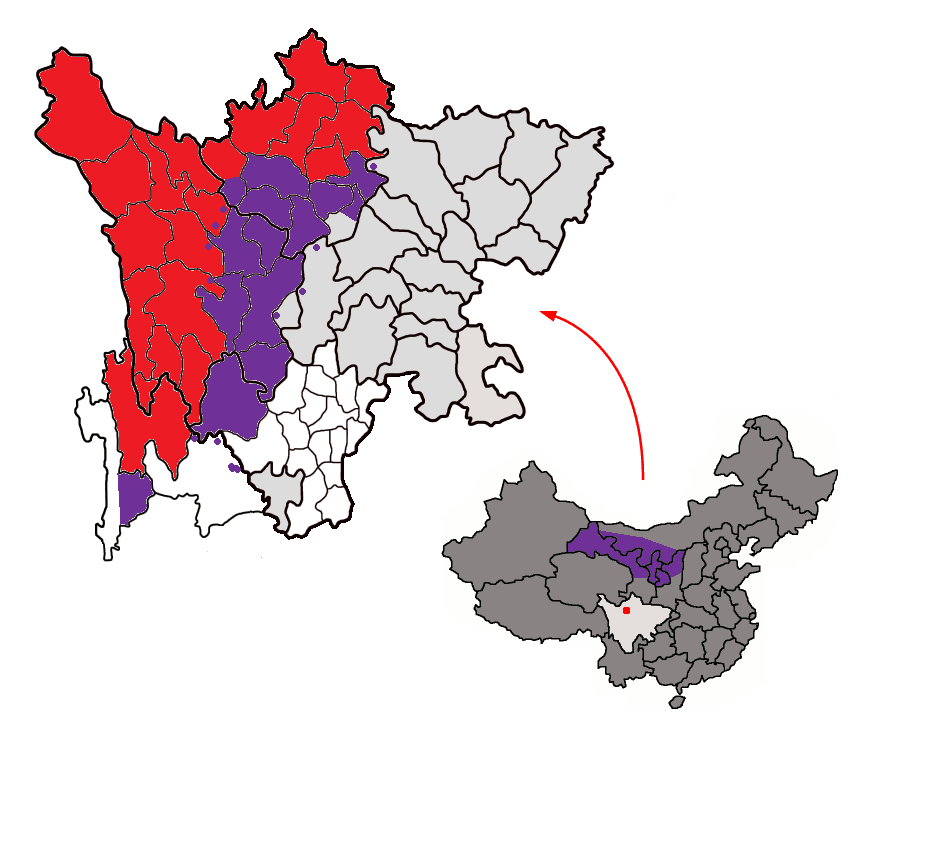
\includegraphics[height=140mm]{qiangic.png}
\caption{Répartition des langues macro-rgyalronguiques}
\label{fig:qiangic}
\end{figure}
	La carte ci-dessus est une représentation simplifiée de la répartition des langues macro-rgyalronguiques, qui y sont indiquées en violet. Les régions tibétaines  où aucune langue de ce groupe n’est parlée sont en rouge. Les langues difficiles à classer, telles que le shixing, le ersu et le namuyi, n’ont pas été incluses parmi les langues macro-rgyalronguiques sur cette carte.
\begin{figure}[h]
\centering
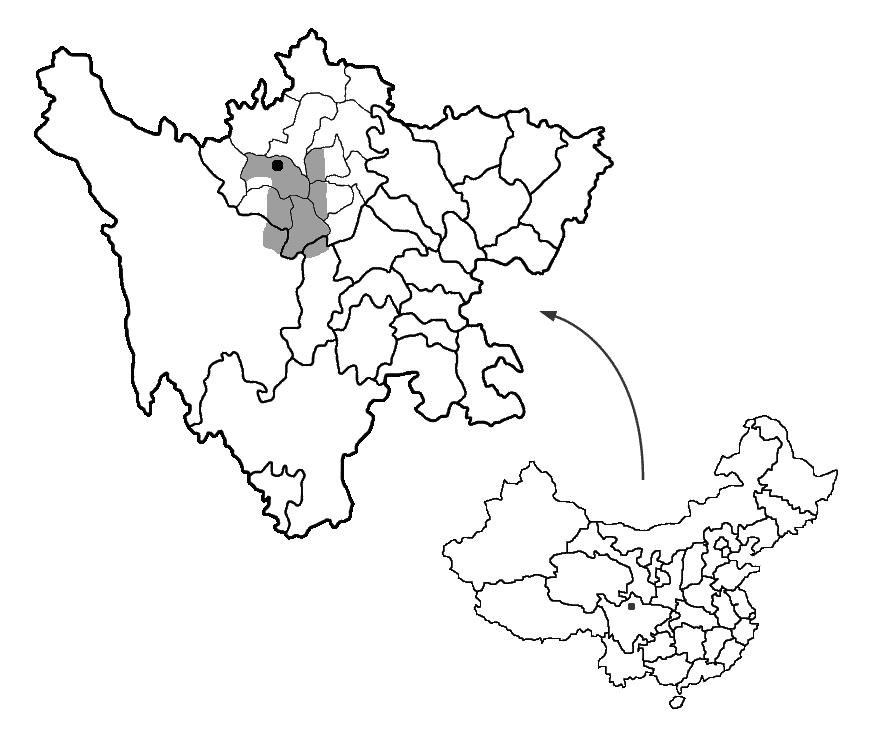
\includegraphics[height=100mm]{carte.JPG}
\caption{Répartition des langues rgyalrong actuelles}
\label{fig:rgyalrong}
\end{figure}
Les langues rgyalrong sont remarquables à plus d’un titre. Contrairement à la majorité des langues sino-tibétaines, elles sont polysynthétiques et présentent une morphologie verbale complexe. De nombreux phénomènes de morphologie non-concaténative, tels que l’apophonie et l’insertion d’infixes, y sont courants. Certaines langues comme le zbu présentent des phénomènes d'alternances polaires (des règles du type $A \rightarrow B$ et $B \rightarrow A$), d'un intérêt considérable pour la typologie linguistique.


Du point de vue de la typologie syntaxique, les langues rgyalrong sont aussi d’une importance capitale, car ce sont les seules de l’Ancien Monde à avoir développé un authentique système d’accord direct / inverse basé sur la hiérarchie d’empathie (\citealt{jacques10inverse}). Elles font partie des rares langues au monde dans lesquelles un alignement casuel ergatif se combine avec un marquage inverse sur le verbe.


Par ailleurs, en ce qui concerne la linguistique historique, elles sont d’un grand intérêt pour la reconstruction du sino-tibétain. En effet, elles font partie des rares langues de cette famille qui semblent préserver les groupes de consonnes initiaux anciens, et à maintenir les préfixes dérivationnels qui ne sont conservés que sous forme de traces dans des langues mieux connues telles que le tibétain ou le chinois. Finalement, concernant l’étude de la dialectologie tibétaine, les langues rgyalrong sont aussi des témoins précieux qui nous permettent de mieux reconstruire le détail de certains changements phonétiques. J'ai montré dans \citet{jacques06s} en particulier que le --s final du tibétain ancien, qui n'est préservé qu'en rgyalrong, a chuté en deux temps: d'abord en finale absolue, puis dans les mots à final --gs (qui étaient passés à --s).

L'intérêt pour la tibétologie du rgyalrong se manifeste aussi dans le vocabulaire, car ces langues préservent des mots parfois non attestés en tibétain ancien, comme \ipa{βzgɤr} ``retarder'' venant d'une forme *bsgor, passé du causatif non-attesté de \textit{ɴgor} ``être en retard'' (les groupes du type de \ipa{βzg--} avec deux fricatives suivies d'une occlusive ne sont pas attestés dans le vocabulaire natif du japhug, et n'apparaissent que dans les emprunts au tibétain).

Mes études sur le japhug profitent de collaborations avec les autres spécialistes des langues rgyalronguiques, en particulier Jackson Sun et Lin Youjing (Academia Sinica, Taiwan), mais  aussi en France Alexis Michaud et Katia Chrikova (CRLAO), dans le cadre du projet ANR PASQi (Phylogenetic Assessment of Southern Qiangic languages) 

Ma publication principale sur le rgyalrong est \citet{jacques08} une grammaire de référence du japhug publiée en chinois aux éditions Minzu chubanshe (Minority Publishing House) à Pékin dans la série ‘Xin faxian yuyan yanjiu congshu’ (Langues minoritaires récemment découvertes) dirigée par Sun Hongkai. Cet ouvrage reprend une partie de ma thèse, mais plus d’un tiers du livre comporte des données inédites, sur des sujets non abordés dans la thèse tels que la complémentation, les idéophones, les classificateurs et la morphologie nominale. Outre une grammaire de la langue, cet ouvrage comprend un étude approfondie de la phonologie et de la morphologie historique du japhug, et notamment une reconstruction des alternances vocaliques dans le système verbal.


Ce livre comprend également deux histoires glosées ainsi qu’un glossaire de plus de deux mille mots. Le choix du chinois comme langue de rédaction de cet ouvrage a été motivé par l’espoir que ce livre puisse rendre service aux locuteurs natifs de la langue, et être plus accessible aux linguistes de Chine. Ce livre ne représente toutefois qu’une petite fraction de l’ensemble de mon travail, car j’ai dû en limiter la taille pour satisfaire aux contraintes de l’éditeur.

Mon autre ouvrage d'importance concernant les langues rgyalrong est \citet{jacques10gesar}, un recueil de textes japhug glosés et commentés. C'est le premier recueil de ce type a être publié non seulement pour le japhug, mais pour quelque langue rgyalrong que ce soit. Les seuls autres textes glosés publiés dans une langue rgyalrong sont deux courtes histoires en annexe de \citet{linxr93jiarong}, et dont le glosage  présente un découpage incorrect des mots.

Outre ces ouvrages, j’ai produit des articles sur des aspects spécifiques de la syntaxe et de la phonologie du japhug. 

	Dans le domaine de la phonologie, j’ai montré dans plusieurs articles comment la réduplication en japhug pouvait être utilisée pour analyser la structure syllabique de cette langue: \citet{jacques04redupl} et \citet{jacques07redupl}.
	
	
	En morphosyntaxe, mes recherches ont porté sur l’actance. J’ai publié un article sur le passif en japhug (\citealt{jacques07passif}) dans lequel j'explique les alternances particulière du morphème de passif a-- et ses relations avec le réciproque. Dans \citet{jacques10refl}, je montre que le préfixe de réfléchi \ipa{ʑɣɤ}-- < *wjaŋ provient de l'incorporation du pronom de troisième personne dans le complexe verbal. Cette innovation propre aux langues rgyalrong est corrélée avec l'absence d'un suffixe cognat avec le --\ipa{si} réfléchi du kiranti.
	
	J'ai écrit un autre article sur le marquage inverse, dans une perspective typologique comparée avec les langues algonquiennes et le kutenai (\citealt{jacques10inverse}). Avec \citet{jackson02rentongdengdi}, ce travail est l'un des premiers à documenter le fonctionnement de l'obviation en rgyalrong.   \citet{gongxun14agreement} a appliqué la même méthodologie pour analyser le marquage personnel en rgyalrong zbu. 
	
Ensuite, dans l'article \citet{jacques12demotion}   je passe en revue les différents procédés dont dispose le japhug pour supprimer un argument. En effet, contrairement aux langues européennes où l'élision d'un objet indique (pour les verbes labiles) un objet indéfini, en rgyalrong comme dans la plupart des langues ST il indique un objet défini. Pour avoir un indéfini, on a un choix différent selon que l'argument supprimé est agent ou patient. Dans le premier cas, on peut choisir entre générique et passif/anticausatif, tandis que dans le second, on a un choix entre quatre formes différentes: générique, antipassif, labilité et incorporation. On trouve également un préfixe dé-expérienceur, par lequel l'actant unique d'un verbe intransitif, ou l'agent (=expérient) d'un verbe de perception se voit supprimé, et remplacé par le stimulus (par exemple \ipa{scit} ``être content'' $\rightarrow $ \ipa{sɤscit} ``être agréable (être tel que les autres sont contents)'').
	
	Les points importants typologiquement de cette étude sont au nombre de trois. Premièrement, le marquage du générique suit un alignement ergatif, et le générique du A est en fait le marqueur d'inverse, ce qui sous-entend une hiérarchie d'empathie dans laquelle la personne générique est plus basse que les inanimés. Deuxièmement, l'antipassif présente une opposition entre patient humain et non-humain (cette découverte est due à \citet{jackson06paisheng} pour le tshobdun). Troisièmement, la labilité en japhug suit un alignement cette fois accusatif (à préservation de l'agent), alors que le marquage des syntagmes nominaux et du générique sont ergatifs. 
	
	J'ai également publié \citet{jacques12incorp} sur l'incorporation   \citet{jacques13harmonization} sur le mouvement associé, \citet{jacques13tropative} sur l'applicatif et le tropatif et \citet{jacques14antipassive} sur l'antipassif. Ces quatre articles, s'ils présentent de nouvelles données, sont aussi des contributions à la typologie morphosyntaxique générale, et seront traités dans la section \ref{chap:typologie}. 
	
	Par ailleurs, un article sur les ideophones en japhug vient d'être accepté par Anthropological Linguistics (\citealt{japhug14ideophones}).
	
	J'ai soumis à plusieurs des travaux sur les constructions comparatives, les relatives et je compte préparer un article pour la section ``Illustrations of the IPA" du \textit{Journal of the IPA}.
	
	Mon travail de documentation futur sur le japhug va porter sur trois aspects:  textes,  dictionnaire et grammaire de référence.
	
\subsection{Textes}
J’ai déjà rendu accessibles huit textes japhug glosés, traduits et alignés avec le fichier sonore sur l’archive du LACITO:
	
	{http://lacito.vjf.cnrs.fr/archivage/index{\underline{  }}fr.htm}
	
De nombreux autres textes ont déjà été analysés et attendent d’être mis en ligne. Idéalement, les textes devraient être tous glosés et traduits en chinois et en français, et j'ai le projet à long terme de traiter les textes progressivement. Je dispose de catégories de textes assez différentes. Je dispose en tout d'environ 30h de textes (chiffre qui ne compte pas les élicitations), dont près de 40h sont déjà transcrites et 5h traduites. Celles qui sont transcrites sans traductions sont néanmoins pourvues de notes pour tous les passages difficiles.


Premièrement, des contes et des mythes, racontés par cinq locuteurs différents (Chen Zhen, sa mère, son oncle, Kubzang 'tsho et Dpalcan).

Deuxièmement, des anecdotes et des récits de vie, racontées par Dpalcan, Chen Zhen et une petite fille (Phurba).

Troisièmement, des textes procéduraux par Chen Zhen et Dpalcan, sur les techniques agricoles et la vie quotidienne.

Quatrièmement, deux conversations d'une heure chacune. Ces données ne seront pas archivées, car elles font référence à la vie privée de mes informateurs, mais je me permets d'en tirer des phrases isolées.

Cinquièmement, les \textit{pear story}, enregistrées pour huit personnes différentes.  

Sixièmement, des traductions de petites histoires tirées des manuels d'école primaire. Je n'en ai pour le moment qu'une dizaine, mais j'incite Chen Zhen à en enregistrer davantage.
	
Enfin, pour améliorer ma connaissance active de la langue, j'écris moi-même des histoires en japhug (adaptées des fables d'Esope) et je me les fais corriger (au téléphone) par Chen Zhen. J'ai déjà composé ainsi 45 histoires. J'enregistre  grâce à Skype les corrections de Chen Zhen, qui sont naturellement plus utiles que mes propres productions imparfaites. En 2010, avec Dpalcan, j'ai traduit en japhug les trois premiers chapitres de la vie de Milarépa. Ce n'est pas du tout une histoire connue localement des Rgyalrongois, mais le milieu tibétain ne leur paraît pas exotique et tout se laisse traduire aisément. J'ai ainsi composé le plus long texte suivi dans une langue rgyalronguique: il fait douze pages de long (sans annotations ni traduction). J'espère que ce type de documents pourra donner par la suite les germes d'une littérature par des locuteurs natifs.

	
\subsection{Dictionnaire} \label{dico}
J'ai entrepris un projet de dictionnaire exhaustif du japhug. C'est un des sous-projet de l'ANR-Corpus Himalco (2013-2015), et je compte produire une première version publique en ligne pour 2015.

Ce dictionnaire, rédigé sous Toolbox (mais qui sera édité sous {\LaTeX} au moyen d'un filtre en PERL), recense le plus de phrases d'exemple possible. 


C'est un dictionnaire japhug-chinois avec gloses en français, et un index chinois-japhug. Il contient plus de 5700 entrées, dont plus de 400 comprennent une description <<~encyclopédique~>> des animaux, des plantes et des objets traditionnels (voir l'exemple de ``crossoptilon'' ci-dessous).   A titre illustratif, voici un des textes inclus dans mon dictionnaire, à l'entrée \textit{qarma} ``crossoptilon'':

\begin{figure}[H]
\centering
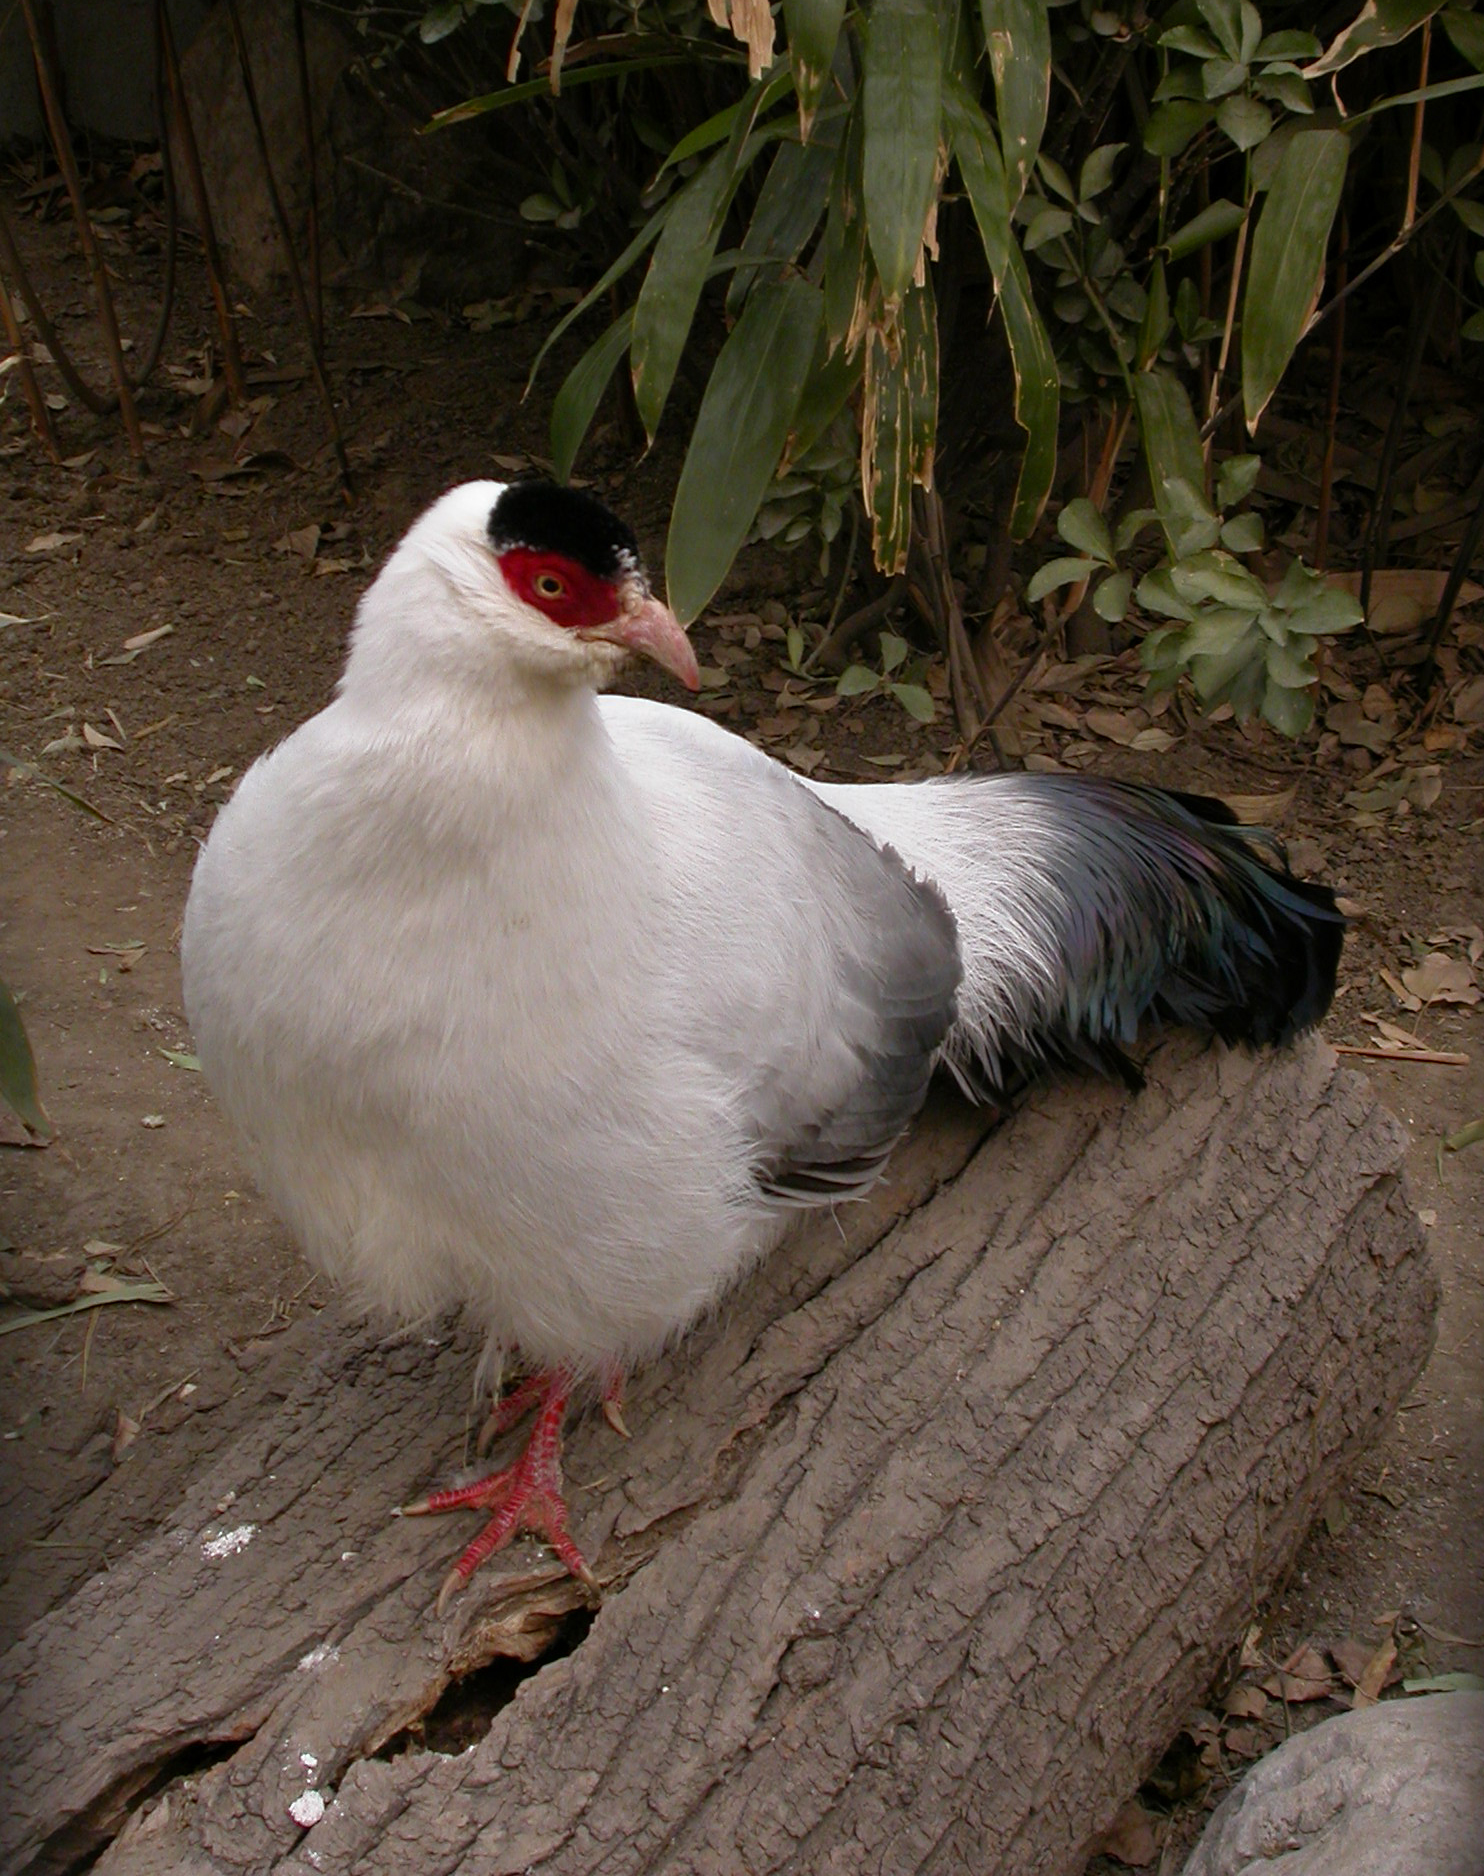
\includegraphics[height=100mm]{WhiteEaredPheasant.jpg}
\caption{qarma ɣrum}
\label{fig:rgyalrong}
\end{figure}

\begin{itemize}


\item qarma nɯ ʁnɯ-tɯphu tu, kɯ-ɲaʁ ci tu, qarma ɲaʁ rmi, tɕe kɯ-wɣrum ci tu, qarma ɣrum rmi. qarma nɯ ɯ-ku ɲaʁ, ɯ-mɲaʁ ɯ-rkɯ nɯ ɣɯrni, ɯ-rna nɯ ɯ-rme ŋgɯ ku-raʁ ʑo ŋu,  kɯ-ɤrqhi ju-kɯ-ru mɤ-saχsɤl, ɯ-jme rɲɟi, qarma ɲaʁ nɯ ɯ-ʁar ku ɲaʁ, ɯ-jme ɯ-kɯ-ɲaʁ dɤn, ɯ-mi qarŋe. qarma ɣrum nɯ kɯ-maʁ ra naχtɕɯɣ, ɯ-ʁar lonba ɣrum, ɯ-jme ɯ-kɯ-ɲaʁ rkɯn. ɯ-mi li kɯ-qarne ŋu. sɯŋgɯ wuma ʑo ku-rɤʑi-ndʑi ɕti. nɯ-ɕpaʁ tɕe, qarma kɯβdɤsqi kɯmŋɤsqi jamar tɯ-tɯ-rca co zɯ kɯ-nɯci pjɯ-ɣi-nɯ ŋgrɤl. qarma nɯ pɣa kɯ-wxti ci ɕti tɕe, tɯ-rdoʁ kɯ sqamŋu tɯ-rpa jamar kɯ-zɣɯt tu, ɯ-ŋgɯm kɯ́nɤ kɯmpɣa ŋgɯm sɤs wxti, qajɯ cho sɯmat ra tu-ndze ɲɯ-ŋu, tɤrɤku ra  li ɣɯ-tu-ndze ngrɤl. tu-mbri tɕe, ɯ-mtɕhi tu-mbri ɯ-rca ɯ-mphɯz kɯ́nɤ tu-mbri ŋu, xɕiri kɯ tu-ti tɕe, 'a-pi qarma ɯ-ɕa mɯm ri, tɯ-sɤtɕha ɲɯ-kɯ-sɯ-spɤr ŋu' tu-ti ɲɯ-ŋgrɤl ma qarma lɤ-zo tɕe xɕiri kɯ ɯ-mke ku-ndɤm tɕe mɯ-ɲɯ-te tɕe, qarma ɲɯ-nɯqambɯmbjom tɕe phɤri ʑo ku-nɯɕe tɕe xɕiri tɤ-rcɯ-rca ku-tsɯm ɲɯ-ŋgrɤl, xɕiri kɯ nɯ kɯ́nɤ mɯ-ɲɯ-te tɕe núɣndʐa nɯ tu-ti ɲɯ-ŋu.


\item Il y a deux espèces de crossoptilon, un noir qui s'appelle crossoptilon noir, un blanc qui s'appelle crosdes dsoptilon blanc. Le crossoptilon a la tête noire, du rouge au bord des yeux, ses oreilles sont à l'intérieur des ses plumes et on ne le voit pas de loin. Sa queue est longue. Le crossoptilon noir a le bout des ailes noir, et il y a beaucoup de noir sur sa queue, les pattes jaunes. Le crossoptilon blanc est pareil que l'autre, ses ailes sont toutes blanches, et il y a peu de noir sur sa queue. Ses pattes sont aussi jaunes. Les deux vivent en forêt. Quand ils ont soif, les crossoptilons viennent à quarante ou cinquante ensemble pour boire. 

Le crossoptilon est à peu près grand comme un poulet, il peut atteindre environ quinze livres, ses œufs sont un peu plus grands que ceux des poules. Il mange des vers et des fruits, et il vient manger les récoltes. Quand il chante, sa queue chante en même temps que la bouche. La belette dit:``La chair du grand frère crossoptilon est bonne à manger, mais à cause de lui, on quitte son propre lieu de villégiature", car lorsque le crossoptilon se pose et la belette l'attrape au cou sans le lâcher, le crossoptilon s'envole, part de l'autre côté de la montagne et emmène en même temps la belette, mais la belette ne lâche pas malgré tout, dit-on.
\end{itemize}

Un tel texte, outre le fait qu'il illustre un grand nombre de formes grammaticales distinctes, présente un intérêt ethnologique évident en cela qu'il documente le savoir traditionnel concernant la faune et la flore locale, ainsi que certaines contes  portant sur ces animaux et plantes. 

Pour les verbes, j'ai systématiquement plusieurs exemples de phrases, parfois une courte définition en japhug, et des liens vers les mots apparentés. A titre d'exemple, voici l'entrée du verbe intransitif ``geler'' (traduite en français, l'original est en chinois):

\begin{exe}
\ex \textit{jpɣom},	\textit{Vi}, dir. \textbf{kɤ-} ``geler''  
\glt \textit{ɕɤfɕo ɲɤ-mɯɕtaʁ tɕe tɯci ko-jpɣom} \\
   Le temps s'est refroidi ces jours-ci, l'eau a gelé. \\
\glt  \textit{jaŋjy ɯ-pɕi pjɤ-kɤ-ta pjɤ-mɯɕtaʁ tɕe pjɤ-jpɣom} \\
  La pomme de terre était dehors, et comme il faisait froid elle a gelé. \\
\glt  \textit{nɤki ɯ-pɕi ma-nɯ-tɯ-te ma ɲɯ-mɯɕtaʁ tɕe jpɣom} \\
  Ne met pas ça dehors, sinon ça va geler! \\
  
  \glt cf. \textit{tɤjpɣom}
\end{exe}
Pour chaque verbe, toutes les informations nécessaires à sa conjugaison sont indiquées: le radical nu (forme qui n'existe pas toujours de façon indépendante de la langue, mais correspond parfois à la troisième personne singulier du non-passé), la transitivité et le préfixe directionnel, éventuellement les formes irrégulières, puis une définition en français et en chinois et un lien avec le fichier son correspondant aux phrases d'exemple. J'ai ajouté des notes concernant l'usage des mots (différences sémantiques entre synonymes) et, de faire encore incomplète, les constructions syntaxiques avec lesquels le verbe en question est compatible. Suivent ensuite plusieurs phrases d'exemple (au moins une, mais pouvant être assez nombreuses pour certains verbes usuels) et leur traduction en chinois. Enfin, on renvoie aux mots apparentés, comme ici le nom \textit{tɤjpɣom} ``glace''.


	
	Ce travail accapare une grande partie de mon temps de recherche récemment, mais est une étape préliminaire indispensable à la rédaction d'une grammaire de référence. 
	
	En effet, une grammaire de référence, contrairement à un sketch grammatical, doit dans la mesure du possible non seulement présenter l'ensembles des constructions possibles, mais aussi présenter exhaustivement les procédés morphologiques qui ne sont pas productifs. Par exemple, pour traiter de l'incorporation, il faudra présenter l'ensemble des verbes à incorporation que j'ai mis au jour, et pas seulement quelques exemples. 
	
	Par ailleurs, il est certain que l'existence d'un dictionnaire est la priorité absolue pour les locuteurs. Si l'existence d'un dictionnaire en soit n'est pas forcément d'une grande utilité pour préserver une langue, c'est en revanche une condition absolue pour le faire. Je tiens donc à le compiler avec le plus grand soin possible.  
	
 
	
	
\subsection{Grammaire de référence du japhug}	 \label{grammaire}
La morphosyntaxe est traitée de façon incomplète dans \citet{jacques04these} et \citet{jacques08}, et malgré un certain nombre d'articles plus récents comme \citet{jacques10inverse}, \citet{jacques12incorp}, \citet{jacques12demotion},    \citet{jacques13harmonization} ou \citet{jacques14antipassive}, il est nécessaire d'approfondir mes analyses et collecter plus de données.

Naturellement, j'ai besoin de finir tout d'abord mon dictionnaire. Quand cette première tâche sera achevée, je pourrai plus systématiquement combiner les phrases d'exemples du dictionnaire avec mes textes comme corpus pour faire un inventaire le plus complet possible des constructions syntaxiques.  

En même temps que je rédige mon dictionnaire, je note les phrases intéressantes dans un brouillon, et j'appelle Chenzhen de façon hebdomadaire pour lui poser des questions sur des points précis, soit pour obtenir des exemples de phrases additionnels, soit pour préciser certaines formes (tel verbe est-il transitif, intransitif ou labile), soit pour m'assurer du sens précis de certaines phrases dans les textes sur lesquelles j'étais passé un peu vite -- il n'y a pas pire erreur que de croire comprendre la structure d'une phrase alors qu'on a commis un contre-sens. Je préfère parfois poser des questions évidentes que de risquer de garder une erreur. Surtout, ces appels me permettent simplement de discuter de sujets variés dans la langue, afin de corriger mes fautes de langue et ainsi de parfaire ma connaissance de la syntaxe.

Cette possibilité de téléphoner compense partiellement la difficulté de l'accès au terrain. Chaque appel est très productif et me demande parfois trois ou quatre heures pour être découpé et analysé.  

Dans sa version actuelle, le brouillon de ma future grammaire de référence comprend seize parties.  J'ai commencé à l'écrire en anglais, car les typologues et les linguistes spécialistes d'autres familles de langues comprennent rarement le français et encore moins le chinois. Comme cet ouvrage n'aura de toutes façons qu'un intérêt ténu pour les locuteurs natifs, il n'est pas grave de l'écrire dans une langue à laquelle ils n'ont pas accès.  

Avant de publier une version finale de cette grammaire, je compte écrire les chapitres sous forme d'articles séparés, les soumettre à plusieurs revues, et de bénéficier ainsi de relecture par les pairs pour améliorer la clarté et la complétude de mes données. J'ai déjà soumis un article sur les relatives (\citet{jacques14relatives}), et je prépare un autre sur la coordination. Je compte en 2014 écrire quatre articles:   sur la complémentation, sur le générique, sur le temps-aspect-mode et sur la phonologie.

\section{Kiranti}
Depuis 2011, j'ai entamé un nouveau projet de recherche sur le khaling, langue kirantie du Népal. Il est possible que je travaille, en collaboration avec Aimée Lahaussois, sur d'autres langues kiranties, en particulier le koyi, mais   de façon moins intensive.

Pour le khaling, la situation sociologique et le rapport aux informateurs est très différente de celle que j'ai rencontrée en Chine. Il existe déjà un système d'écriture très imparfait créé par des missionnaires, mais qui ne convient pas aux khalingophones non-chrétiens. Ils recherchaient donc un linguiste  capable de concevoir une orthographe et de les aider à compiler un dictionnaire, afin de disposer d'un système d'écriture représentant l'ensemble des distinction phonologiques, et évitant certains graphèmes qu'ils associent aux missionnaires. 

Les khalings sont très actifs et davantage motivés que les locuteurs du japhug pour protéger leur langue. Ils écrivent des chansons, des recueils de poèmes, et se communiquent couramment en khaling par messagerie électronique (facebook, email, SMS etc). Ils sont également plus exigeants quant à mes travaux, et sont soucieux de ne pas publier notamment des histoires qu'ils ne jugent pas ``parfaites", ce qui complique la compilation d'un corpus oral.

Dans ces conditions, étant donné mon travail sur le japhug qui occupe une grande partie de mon temps, et la nécessité d'ajouter le népali dans le dictionnaire (langue dont je n'ai que des notions limitées, surtout en langue orale), il m'a semblé plus réaliste de me concentrer pour les trois années suivantes (dans le cadre de l'ANR Himalco) à un projet plus restreint que celui commencé pour le japhug: compiler exclusivement un dictionnaire de verbes, combiné à des paradigmes complets. Pour cela j'ai conçu plusieurs scripts PERL pour convertir automatiquement ma base de données Toolbox.

Sur cette langue, mon unique publication pour le moment est \citet{jacques12khaling}, où je présente une reconstruction interne des flexions et une liste complète de paradigmes générés par un script perl, qui m'a permis de revérifier le modèle proposé en soumettant ensuite ce travail à trois locuteurs natifs qui ont relu attentivement tous les tableaux. Cet article sera la base non seulement d'autres travaux en cours de préparation sur d'autres types de conjugaisons (les verbes réfléchis et les verbes bipartites), mais aussi à une modélisation de la morphologie en collaboration avec Sagot et Walther (cf section \ref{sec:paradigms.khaling}).

J'ai en outre préparé une communication invitée ``Derivational morphology in Khaling"   pour un symposium à Seattle en août 2013 (Li Fang-Kuei Society Young Scholars Symposium, \citealt{jacques13derivational.khaling}), dans laquelle je décris quelques phénomènes de dérivation non productive (mais ancienne) et où je montre que l'alternance de voisement liée à la transitivitée en Khaling est apparenté à la prénasalisation anticausative du japhug, et non au préfixe causatif.

Je prépare aussi un article sur un démonstratif auditif en khaling dans une perspective typologique, basé sur des données tirées de conversations naturelles. Il sera resoumis prochainement (il est actuellement en cours de révision).


Dans un avenir plus lointain, je me consacrerai aussi à une grammaire de référence et à un recueil de textes mythologiques, ainsi probablement qu'à la rédaction de matériaux d'enseignement pour les enfants dont le khaling est la langue maternelle.


Dans une perspective typologique, le khaling et les autres langues kiranties présentent tout autant d'intérêt que le rgyalrong, mais dans des domaines différents. Alors que les langues rgyalrong on un système de dérivation par préfixes  d'une grande richesse, les langues kiranties ont plutôt développé des prédicats complexes à partir de constructions en série. Ceux-ci sont partiellement transparents étymologiquement, mais présentent des alternances vocaliques sans équivalents ailleurs, et leur genèse exacte est compliquée. Ils illustrent des chemins de grammaticalisation parfois peu habituels (``manger" $\rightarrow$ permansif), et présentent la particularité de conserver les marques de personnes à la fois de l'auxiliaire et aussi du verbe primaire, qui subissent néanmoins certaines opérations morphologiques particulières; on a ainsi des formes verbales doublement conjuguées. La même personne peut donc dans certains cas être marquée par quatre marques différentes dans la même forme verbale.


La structure des paradigmes kirantis est d'un intérêt typologique pour leur grande opacité en comparaison avec ceux du rgyalrong. Par exemple, le préfixe \ipa{ʔi--} du khaling se retrouve aux formes \textsc{2intr}, 2>3, 3>2, 1dp>2, 2>1, 3>1, comme l'illustre le tableau suivant:

\begin{table}[H]
\caption{Paradigme transitif du khaling}\label{tab:jpg.tr}
\resizebox{\columnwidth}{!}{
\begin{tabular}{l|l|l|l|l|l|l|l|l|l|l|l|}
\textsc{} & 	\textsc{1s} & 	\textsc{1di} & 	\textsc{1de} & 	\textsc{1pi} & 	\textsc{1pe} & 	\textsc{2s} & 	\textsc{2d} & 	\textsc{2p} & 	\textsc{3s} & 	\textsc{3d} & 	\textsc{3p} \\ 
\hline	
\textsc{1s} & 	\multicolumn{5}{c|}{\grise{}} &	\ipa{R-nɛ}   &	\ipa{R-su}   &	\ipa{R-nu}   &	\ipa{R-u}   &	\ipa{R-u-su}   &	\ipa{R-u-nu}   \\	
\cline{7-12}
\textsc{1di} & \multicolumn{8}{c|}{\grise{}} &	\multicolumn{3}{c|}{	\ipa{R-i} }	   \\	
\cline{7-12}
\textsc{1de} & 	\multicolumn{5}{c|}{\grise{}} &	\ipa{ʔi-R}   &	\ipa{ʔi-R-i}   &	\ipa{ʔi-R-ni}   &	 \multicolumn{3}{c|}{	\ipa{R-u} }	   \\	
\cline{7-12}
\textsc{1pi} & 	\multicolumn{8}{c|}{\grise{}} &	 \multicolumn{3}{c|}{\ipa{R-ki}}   \\	
\cline{7-12}
\textsc{1pe} & 	\multicolumn{5}{c|}{\grise{}} &	\ipa{ʔi-R}   &	\ipa{ʔi-R-i}   &	\ipa{ʔi-R-ni}   &\multicolumn{3}{c|}{\ipa{R-kʌ} }	   \\	
\cline{2-2}
\cline{4-4}
\cline{6-12}
\textsc{2s} & 	\ipa{ʔi-R-ŋʌ}   &	\grise{} &	   &	\grise{} &	   &	\grise{} &	\grise{} &	\grise{} &	\ipa{ʔi-R-ʉ}   &	\ipa{ʔi-R-su}   &	\ipa{ʔi-R-nu}   \\	
\cline{2-2}	
\cline{10-12}
\textsc{2d} & 	\ipa{ʔi-R-ŋʌ-su}   &	\grise{} &	   &	\grise{} &	   &	\grise{} &	\grise{} &	\grise{} &	 \multicolumn{3}{c|}{\ipa{ʔi-R-i} }	   \\	
\cline{2-2}	
\cline{10-12}
\textsc{2p} & 	\ipa{ʔi-R-ŋʌ-nu}   &	\grise{} &	   &	\grise{} &	   &	\grise{} &	\grise{} &	\grise{} &	\multicolumn{3}{c|}{\ipa{ʔi-R-ni}}	   \\	
\cline{2-3}	
\cline{5-5}	
\cline{7-12}
\textsc{3s} & 	\ipa{ʔi-R-ŋʌ}   &	   &	   &	   &	   &	   &	   &	   &	\ipa{R-ʉ}   &	   &	   \\	
\cline{2-2}	
\cline{10-10}
\textsc{3d} & 	\ipa{ʔi-R-ŋʌ-su}   &	\ipa{ʔi-R-i}   &	\ipa{ʔi-R-u}   &	\ipa{ʔi-R-ki}   &	\ipa{ʔi-R-kʌ}   &	\ipa{ʔi-R}   &	\ipa{ʔi-R-i}   &	\ipa{ʔi-R-ni}   &	  \multicolumn{2}{r|}{\ipa{R-su}}   &	   \\	
\cline{2-2}	
\cline{10-11}
\textsc{3p} & 	\ipa{ʔi-R-ŋʌ-nu}   &	   &	   &	   &	   &	   &	   &	   &	   \multicolumn{3}{r|}{\ipa{R-nu}   } \\	
\hline
\end{tabular}}
\end{table}



Il s'agit donc de toutes les formes inverses, plus les formes de deuxième personne à l'exception de 1s>2. Il s'agit certainement de la fusion de deux préfixes distincts (inverse et seconde personne), mais la genèse de ce préfixe et le chemin  par lequel un tel système en est venu à se mettre en place est peu clair.

\section{Autres langues sino-tibétaines étudiées} 
Outre le japhug et le zbu, j'ai travaillé sur plusieurs langues sino-tibétaines, dont le pumi du nord, le tibétain de Cone, mais aussi à moindre mesure chang naga et le konyak de Tanhai. Outre ces langues, j'ai pu travaillé très brièvement avec des locuteurs de khengkha (au Bhoutan) de yongyimchin et de tangkhul (Nagaland) et aussi de muya, de guiqiong, de rgyalrong de l'est, de tshobdun, de khroskyabs et de rtau (parmi les langues qianguiques). A Paris, j'ai pris contact avec un locuteur du Minyag, Ngag.dbang Don.grub, et un locuteur du resnyeskad, Lobsang Nyima.

Les seules langues macro-rgyalronguiques sur lesquelles je n'ai jamais travaillé sont le Zhaba, le Queyu, le Stodsde et le khroskyabs de Njorogs (Yelong).


Je n'ai pas effectué encore de terrain approfondi sur des langues en dehors du sino-tibétain, mais j'étudie les langues algonquiennes en parallèle à mes travaux sur le sino-tibétain.

\subsection{Pumi}
J'ai effectué deux séjours de terrain sur le pumi, en juillet-août 2008 (à Yongning, Ninglang, Yunnan) et en février-mars 2009 (à Muli, Liangshan, Sichuan), sur les dialectes de Mudiqing et de Shuiluo respectivement dans le cadre de l'ANR PASQi. 

Le premier séjour au Yunnan a eu lieu dans une région majoritairement de langue Na. J'ai habité dans la maison de Latami, l'informateur de mon collègue Alexis Michaud, et j'ai travaillé avec monsieur Cao, un locuteur du pumi de Mudiqing. Cette variété, parlée autrefois au nord de Yongning, est particulièrement menacée car le village a été déplacé pour construire un réservoir d'eau, et que l'alcoolisme sévit de façon grave parmi les gens originaires de ce village. Le pumi de Mudiqing a un système vocalique particulièrement complexe que mon court séjour de terrain ne m'a pas permis d'élucider en détail.

Le second séjour, en 2009, s'est déroulé en compagnie d'Alexis Michaud et Katia Chirkova. Nous avons été malheureusement renvoyés de Muli au bout de trois semaines, mais ce temps fut suffisant pour déterminer le système phonologique de cette langue et analyser deux   histoires de longueur moyenne (en tout plus de 20 minutes d'enregistrement). La variété de Shuiluo est particulièrement intéressante par la présence de fricatives aspirées. Contrairement au pumi de Mudiqing, qui est en contact avec le na, le pumi de Shuiluo est en contact avec le shixing et le tibétain Kami.
 

Les principales retombées immédiates de ce terrain sont d'une part mon article sur les alternances tonales dans le verbe (\citealt{jacques11pumi.tone}), où je montre qu'au delà de certaines similarités avec le Shixing (\citealt{chirkova09tone}) et le na (\citealt{michaud08na}), le pumi du nord présente des alternances qui ne peuvent s'expliquer que par l'hypothèse que les monosyllabes comportent quatre catégories tonales (et non trois) et les dissyllabes cinq catégories tonales (et non quatre), comme le montrent les deux tableaux \ref{fig:pumi01} et \ref{fig:pumi01}:

\begin{figure}[h]
\centering
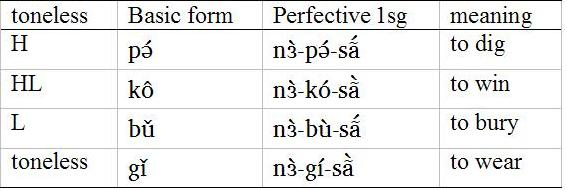
\includegraphics[height=35mm]{pumi01.jpg}
\caption{Verbes monosyllabiques en pumi du nord}
\label{fig:pumi01}
\end{figure}
\begin{figure}[h]
\centering
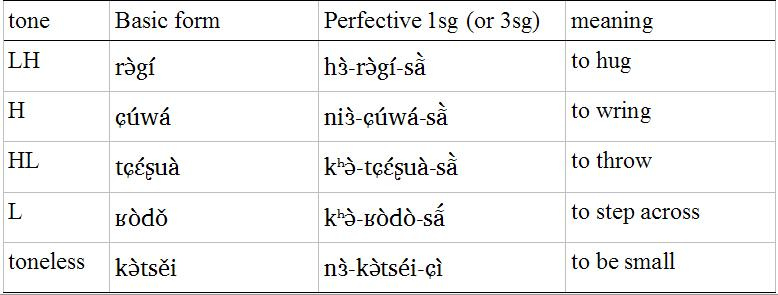
\includegraphics[height=50mm]{pumi02.jpg}
\caption{Verbes dissyllabiques en pumi du nord}
\label{fig:pumi01}
\end{figure}
Les alternances entre ton montant et tombant sont interprétées dans mon travail comme étant de façon sous-jacente une catégorie atonale.

Cette catégorie était inconnue de tous les travaux précédents sur le pumi du nord. Il est d'une importance non-négligeable non seulement pour la phonologie historique, mais également pour la simple description synchronique du pumi.

Mon autre contribution à l'étude du pumi est ma découverte des fricatives aspirées en pumi de Shuiluo (\citealt{jacques11lingua}). Ce travail sera présenté plus en détail en \ref{sec:panchrp} p.\pageref{sec:panchrp}.

Je m'intéresse à la phonologie historique du pumi, mais les données dont je dispose sont insuffisantes pour permettre une étude complète de la phonologie de cette langue. Tout au plus puis-je signaler quelques étymologies inattendues telles que Shuiluo \ipa{nî}, Mudiqing \ipa{nê}, probablement apparenté au japhug \ipa{nŋo} malgré la dissimilitude apparente de ces formes. La forme japhug vient sans aucun doute  de *t-ŋaŋ; or, le --i du pumi de Shuiluo et le --e de celui de Mudiqing, sous leurs formes nasalisées --ĩ et --ẽ, proviennent en parti d'un ancien *--aŋ. Or, devant consonne nasale, les rimes sont toujours nasalisées; Donc, la correspondance vocalique est parfaite. Pour les consonnes initiales, il faut tenir compte du fait que le ŋ-- n'apparaît jamais devant voyelles antérieures dans cette variété de pumi, et que les anciens *ŋ-- et *n-- ont donc été neutralisés dans ce contexte. On peut donc en conclure que ces formes sont cognates, et présentent des correspondances phonétique et sémantique parfaites.

J'ai aussi contribué à \citet{michaud10bonin}, article dans lequel Alexis Michaud et moi-même analysons des transcriptions imparfaites du naxi et du pumi datant du début du siècle dernier à la lumière de nos travaux de terrain.
 


Le pumi est actuellement étudié par au moins trois autres chercheurs, Picus Ding, Henriette Daudey (qui s'apprête à soutenir sa thèse à l'univeristé LaTrobe sous la direction de David Bradley) et Skalbzang Phuntshogs, un locuteur natif  du pumi affilié à la SIL. La description de cette langue doit donc se concevoir dans un contexte collaboratif. On pourra envisager à plus long terme un dictionnaire inter-dialectal basé sur plusieurs parlers. 

\subsection{Tibétain Kami}
Durant mon séjour à Muli sur le pumi en 2009, j'ai également brièvement travaillé sur le tibétain kami. Je n'ai pas pu enregistrer de textes, mais j'ai transcrit plus de sept cents mots et j'ai établi les correspondances entre cette langue et le tibétain ancien. Ces données ont été incorporées par Katia Chirkova à son article sur le Kami qui paraîtra dans le même volume que mon étude du Cone.

\subsection{Tibétain de Cone}

En octobre-décembre 2010, j'ai effectué un court séjour de terrain sur le tibétain de Cone, et je prépare en ce moment une description de la phonologie de cette langue. Cette forme de tibétain présente à la fois des archaïsmes remarquables (la préservation du paradigme irrégulier de ``manger''), mais aussi des innovations phonétiques importantes, et des innovations morphologiques intéressantes (le paradigme du verbe ``faire'' combine des formes de deux étymons distincts, \textit{bʲed} et de \textit{bgʲid}, qui ont phonétiquement convergé).

Sur le plan de la phonologie, le Cone a perdu les groupes de consonnes initiaux et n'a plus que --r parmi les neuf consonnes finales du tibétain ancien. Le système vocalique de cette langue est le suivant:

\begin{table}[H]
\caption{Système vocalique de la langue de Cone}\label{tab:cone1}
\begin{tabular}{lllllllllllll} 
\toprule
i  &  	iː  &  	ʉ  &  	ʉː  &  	u  &  	uː  &  	   &  	   &  	ĩː  &  	   &  	   &  	(ũː)  &  \\
ɪ  &  	ɪː  &  	   &  	   &  	   &  	   &  	   &  	   &  	   &  	   &  	   &  	   &  \\
e  &  	eː  &  	   &  	   &  	o  &  	oː  &  	   &  	   &  	ẽː  &  	   &  	   &  	õː  &  \\
ɛ  &  	   &  	ə  &  	   &  	ɔ  &  	   &  	   &  	   &  	   &  	   &  	   &  	   &  \\
æ  &  	   &  	   &  	   &  	ɑ  &  	ɑː  &  	   &  	   &  	   &  	ã  &  	ãː  &  	   &  \\
  &  	  &  	  &  	  &  	  &  	  &  	  &  	  &  	  &  	  &  	  &  	  &  \\
\bottomrule
\end{tabular}
\end{table}
Unique parmi les langues tibétaines décrites jusqu'à maintenant, le tibétain de Cone a la particularité d'avoir cinq degré de hauteur /i ɪ e ɛ æ./ Aux trois premières voyelles correspondent aussi des  phonèmes vocaliques longs /iː ɪː eː/. J'ai pu déterminer les correspondances suivantes entre le tibétain de Cone et le tibétain ancien pour les voyelles:
\begin{table}[H]
\caption{Correspondances entre tibétain ancien et dialecte de Cone (rimes)}\label{tab:cone}
\begin{tabular}{l|llllllllll} 
\toprule
   &  	Ø  &  	b  &  	d  &  	g  &  	m  &  	n  &  	ŋ  &  	r  &  	l  &  	s  \\
\midrule
a  &  	æ  &  	e  &  	e  &  	a  &  	ã  &  	ẽ  &  	ɑː  &  	ær  &  	ɑː  &  	eː   \\
e  &  	ɛ  &  	ɪ / e  &  	ɪ  &  	a  &  	ẽ  &  	ẽ  &  	eː  &  	er  &  	iː ?  &  	ɪː   \\
i  &  	ə  &  	ʉ  &  	i  &  	i  &  	ĩ  &  	ĩ  &  	iː  &  	ər  &  	iː  &  	iː   \\
o  &  	ɔ  &  	   &  	ɪ  &  	u  &  	õ  &  	ẽ  &  	uː  &  	or  &  	uː  &  	ɪː   \\
u  &  	ə  &  	ʉ  &  	i  &  	ʉ  &  	õ  &  	ĩ  &  	ʉː  &  	ər  &  	ʉː  &  	iː   \\ 
\bottomrule
\end{tabular}
\end{table}
Ces correspondances s'appliquent à la couche héritée du vocabulaire. Je n'ai aucun exemple certain de mot venant --\ipa{ob}. On remarque qu'une suite de changements en chaînes ont eu lieu: 
\begin{itemize}
\item Les voyelles fermées i et u se sont centralisées en [ə]
\item Les voyelles courtes fermées et mi-fermés i ɪ e u ʉ viennent de syllabes fermées en occlusives. 
\item Les voyelles longues correspondantes viennent de syllabes fermées en --ŋ, en --l ou en --s. Contrairement à beaucoup de dialectes, le --s final ne devient pas un coup de glotte et ne donne pas de voyelle courte.
\end{itemize}
Les voyelles nasales proviennent des rimes à finales --m et --n seulement dans la couche héritée.

Les groupes initiaux se sont simplifiés selon les règles suivantes:

\begin{longtable}{l|llllllllll} 
\caption{Correspondances entre tibétain ancien et dialecte de Cone (initiales)}\label{tab:cone3} \\
\toprule
Cone  &  	vocabulaire hérité  &  	emprunté / irrégulier  \\  
\midrule
p¹  &  	(C)Cp  &  	spr  \\  
p²  &  	b  &  	ɴb  \\  
pʰ  &  	(ɴ)pʰ  &  	   \\  
b²  &  	(C)Cb  &  	   \\  
mb²  &  	ɴb  &  	b  \\  
t¹  &  	(C)Ct  &  	   \\  
t²  &  	d  &  	   \\  
tʰ  &  	(N)tʰ  &  	   \\  
d²  &  	(C)Cd  &  	   \\  
nd²  &  	Nd  &  	   \\  
ts¹  &  	(C)Cts, (b)sl  &  	gtɕ  \\  
tsʰ  &  	(N)tsʰ  &  	   \\  
dz²  &  	(C)Cdz, (b)zl  &  	bts  \\  
ndz²  &  	Ndz  &  	   \\  
tɕ¹  &  	(C)Cc  &  	bkr, (C)Ckʲ, dpʲ  \\  
tɕ²  &  	j, gr  &  	   \\  
tɕʰ  &  	(N)ch, (N)kʰr, (N)kʰʲ  &  	pʰʲ  \\  
dʑ²  &  	(C)Cdʑ, (C)Cgʲ &  	   \\  
ndʑ²  &  	Ndʑ, Ngr, Ngʲ, ɴbʲ  &  	   \\  
tʂ²  &  	dr, br  &  	gr, spr  \\  
tʂʰ  &  	(ɴ)pʰr  &  	(N)kʰr  \\  
dʐ²  &  	   &  	Cbr, Cgr  \\  
ndʐ²  &  	ɴbr,Ndr  &  	ɴgr  \\  
k¹  &  	(C)Ck  &  	   \\  
k²  &  	g  &  	   \\  
kʰ  &  	(N)kʰ  &  	   \\  
g²  &  	(C)Cg  &  	   \\  
ŋg²  &  	Ng  &  	rg  \\  
m¹  &  	Cm  &  	   \\  
m²  &  	m  &  	   \\  
n¹  &  	Cn  &  	   \\  
n²  &  	n  &  	   \\  
ɲ¹  &  	Cɲ,Cm(ʲ)e, Cm(ʲ)i  &  	   \\  
ɲ²  &  	ɲ  &  	n, ŋ / -as   \\  
ŋ¹  &  	Cŋ  &  	   \\  
ŋ²  &  	β  &  	   \\  
s¹  &  	Cs  &  	sl, sr  \\  
s²  &  	z  &  	   \\  
sʰ  &  	s  &  	sl  \\  
z²  &  	Cz  &  	   \\  
ɕ¹  &  	(C)Ckr, (C)Ckrʲ, Cpʲ,  &  	Cɕ  \\  
ɕ²  &  	bʲ  &  	Cʑ, spʲ  \\  
ɕʰ  &  	(ɴ)pʰʲ  &  	ɕ  \\  
ʑ²  &  	sbʲ  &  	bʲ, Cʑ  \\  
ʂ¹  &  	sr, spr  &  	Cɕ  \\  
ʂ²  &  	   &  	Cʑ  \\  
ʂʰ  &  	hr  &  	s(Vr)  \\  
ʐ¹  &  	sbr, sgr  &  	   \\  
x¹  &  	Cɕ  &  	dp  \\  
x²  &  	ʑ  &  	   \\  
xʰ  &  	ɕ  &  	Cɕ  \\  
ɣ²  &  	Cʑ  &  	sbʲ  \\  
r²  &  	r  &  	   \\  
l¹  &  	bl, kl, gl, rl  &  	sl  \\  
l  &  	l  &  	   \\  
ɬ  &  	lh  &  	   \\  
j¹  &  	gj, dbʲ  &  	   \\  
j²  &  	y  &  	ɦ  \\  
w¹  &  	?  &  	   \\  
w²  &  	w  &  	sbr, rb  \\  
h  &  	h  &  	pʰ, lh  \\  
\bottomrule
\end{longtable}


J'ai enregistré et analysé trois textes et j'ai recueilli un vocabulaire d'environ 1500 mots.  Outre l'aspect purement descriptif, ce travail est également important pour mon étude des fricatives aspirées, présenté plus en détail en \ref{sec:panchrp} p.\pageref{sec:panchrp}.

\subsection{Naga du nord}
J'ai brièvement travaillé sur les langues naga du nord en Inde (Shillong, Meghalaya et Guwahati, Assam) en 2007. Le but premier de mon travail était de revérifier les données du chang naga de façon à pouvoir rédiger mon article \citet{jacques07chang}, mais j'y ai également travail sur le Tanhai, une langue proche du Wancho encore non documentée. 


\subsection{Minyag}
J'ai brièvement travaillé sur le minyag en 2003 à Chengdu, mais j'ai récemment découvert un informateur à Paris, et espère à plus long terme pouvoir collaborer avec lui pour préparer au moins un recueil de textes, et même éventuellement une grammaire.

J'ai recueilli des données ultrason sur le système vocalique du muya, afin d'étudier le trait ``tendu-relâché" de cette langue, qui semble être une opposition entre voyelles normales et voyelles uvularisées, une opposition phonologique aussi attestée en qiang du nord (voir le travail en cours d'Evans et Sun).

\subsection{Rtau}
En collaboration avec Anton Antonov et de Lai Yunfan, je travaille depuis juin 2012 à Paris sur le Rtau, une langue proche du rgyalrong, avec Lobzang Nyima, un  locuteur de cette langue qui habite en France depuis dix ans. 

Cette recherche a donné lieu à une présentation au troisième \textit{Workshop on the Sino-Tibetan of Sichuan} organisé dans le cadre de l'ANR Himalco en septembre 2013 à l'EHESS sur le système d'accord de cette langue et les alternances vocaliques particulièrement complexes, pour lesquelles nous proposons une analyse.

Nous avons déjà recueilli un glossaire d'un millier de mots et une dizaine d'histoires, et avons le projets d'effectuer des recherches de terrain au Sichuan dans la région où le rtau est parlé.\footnote{Lors de son séjour de terrain à Wobzi (Chuchen, Sichuan, Chine) en février 2014, Lai Yunfan a découvert un autre dialecte du rtau sur lequel il va effectuer des recherches additionnelles.} Nous préparons également des présentations à plusieurs conférences sur le discours rapporté, les emprunts au tibétain et la relativisation en rtau sur la base de ces données.

Les données du Rtau sont également d'une grande utilité pour mes travaux sur la typologie et la diachronie des systèmes direct-inverse en comparaison avec ceux des langues rgyalrong.

\chapter{Linguistique comparée des langues sino-tibétaines}



\epigraph{\textit{La restitution d'une « langue commune » dont le chinois, le tibétain,
etc., par exemple, seraient des formes postérieures, se heurte à des
obstacles quasi invincibles}. Antoine Meillet}

	Les deux précédents domaines d’études  ont en commun l’étude historique des langues sino-tibétaines. Mes recherches m’ont porté à étudier en détail cinq langues de la famille sino-tibétaine: trois langues anciennes (le chinois, le tibétain et le tangoute) ainsi que deux langues modernes mais relativement conservatrices (le japhug et le khaling).  
	
	La linguistique historique est un domaine certes moins urgent  que la description des langues, mais c'est l'un  de ceux qui me tient le plus à cœur. 	Les méthodes de reconstruction des proto-langues et l'étymologie sont parfois reçues avec suspicion par certains linguistes. Ce scepticisme s'explique en partie par le manque de familiarité de beaucoup de linguistes avec les  principes véritables de la linguistique comparée. Pour se convaincre du bien fondé de ces méthodes, il suffit d'écrire un programme appliquant les lois phonétiques régulières connues à des proto-formes (ou les appliquant à l'envers sur des formes modernes).; j'aborderai ce sujet en section \ref{sec:comp.ling.hist}.
	

	
	
L'application de la méthode comparative aux langues sino-tibétaines, tout comme à d'autres familles de langues gigantesques tels que le Niger-Congo et le Mon-Khmer, se heurte à des difficultés considérables. Tout d'abord, seule une infime minorité de ces langues sont décrites suffisamment en détail pour permettre une application valide de la méthode comparative. Toute reconstruction reste donc nécessairement provisoire tant que de meilleures données ne sont pas disponibles.

La difficulté vient également de la profondeur temporelle abyssale qui nous sépare de la proto-langue, et de la variété extraordinaire des langues actuelles. D'autre part, les langues isolantes de la famille sino-tibétaine sont particulièrement difficiles à étudier dans une perspective comparative. Comme l'avait soulevé Meillet il y a plus d'un siècle, dans le cas de langues à morphologie pauvre, il est difficile de distinguer traits empruntés et hérités. Néanmoins, il ignorait tout à l'époque des langues à morphologie riche de la famille, qui ne commencent à être décrites que depuis une trentaine d'années. 

Un problème additionnel, enfin, porte sur les limites de la famille sino-tibétaine. Même si plus personne ne doute que le chinois appartient à cette famille, on trouve un nombre important de langues de l'Inde du nord-est telles que le sulong dont il est difficile de dire si ce sont des langues sino-tibétaines ayant subi des changements phonétiques au point de devenir méconnaissables, ou des langues de chasseurs-cueilleurs isolées mais fortement influencées par des langues sino-tibétaines. 


\section{Phonologie comparée}
Mon travail se distingue des précédentes études comparatives telles que \citet{peiros96st}, \citet{gong95st} et \citet{matisoff03} par la méthodologie employée. Contrairement à ces auteurs en effet, j’ai cherché à ne pas  effectuer de simples comparaisons lexicales, mais à analyser dans chaque langue des exemples de l'usage des mots comparés dans les textes les plus anciens afin d’être certain de leur sens et de leur usage grammatical exact en contexte dans chacune des langues comparées. Cette méthode permet de rejeter de nombreuses comparaisons convaincantes au premier abord. 


Par exemple, le terme tibétain \textit{gɕags} ‘confession’ (dérivé du verbe \textit{bɕags} ‘se confesser’) est parfois comparé au chinois \zh{色} *s^{ʕ}rək ‘honte’. Cette comparaison est acceptable du point de vue des correspondances phonétiques (le chinois archaïque *sr- et *-ək correspond bien au tibétain ɕ- et -ag). Toutefois, un examen philologique plus fin révèle que cette comparaison est erronée: le verbe  \textit{bɕags} signifie en effet ``déclarer'' dans son attestation la plus ancienne, l’inscription bilingue sino-tibétaine de 822, et non pas ``se confesser''. Il s’agit en fait d’un sens secondaire apparu après la conversion du Tibet au bouddhisme.


Sur la base de ces connaissances, j’ai conçu une base de données comparative comprenant cinq langues (rgyalrong, tangoute, chinois, tibétain et limbou) qui pourra servir de base à un futur dictionnaire étymologique du sino-tibétain. De cette base de données, seule pour le moment a été présentée une communication succincte sur les cognats entre rgyalrong et chinois archaïque (\citealt{jacques05} déjà cité plus haut). Dans cette communication, je montre que le rgyalrong et le chinois ont en commun deux étymons pour <<~ours~>>, l'un pour l'ours brun et l'autre pour l'ours noir. A moins que des emprunts ne soient responsables de ces isoglosses, cela impliquerait que l'Urheimat sino-tibétaine soit située dans une région où les aires de répartition des deux ours se croisent; en Chine actuelle, ces zones ne se croisent qu'en Mandchourie et au Tibet: il faudrait déterminer jusqu'où s'étendait cette zone au néolithique tardif.


J'ai par ailleurs collaboré avec Alexis Michaud sur l'étude de la phonologie historique des langues naish (\citealt{jacques.michaud11naish}). Dans ce travail, nous avons en particulier montré que l'évolution des voyelles dépend non seulement des consonnes qui suivent, mais également de celles qui précèdent. Les changements phonétiques sont considérables, mais au moins pour les rimes en syllabe ouverte, les correspondances sont très claires. L'article est basé sur une méthodologie consistant à déterminer si les correspondances entre les trois langues Naxi, Na et Lazé sont en distribution complémentaires par rapport aux initiales. A partir de ces distributions complémentaires, on regroupe des correspondances apparemment sans rapport (telles que e:ie:i et ɯ:ɯ:i) sous une même reconstruction dans la proto-langue. Le *a du proto-na est particulièrement complexe: il présente sept réflexes distincts selon la consonne initiale. 

Ce travail est à la fois une contribution au comparatisme sino-tibétain, et à la méthodologie de la reconstruction.

\section{Morphologie comparée}
	Un autre aspect du travail de recherche sur l’histoire du sino-tibétain concerne la morphologie. Les travaux sur la reconstruction de la morphologie en sino-tibétain publiés jusqu’ici ont souffert de deux défauts importants: tout d’abord, pour la plupart d’entre eux, aucune attention n’a été portée aux correspondances phonétiques, si bien que les <<~reconstructions~>> proposées sont le plus souvent peu rigoureuses. L’autre problème est que ces reconstructions négligent l’étude de la morphologie irrégulière commune, et se contentent se comparer des formes régulières qui pourraient résulter de nivellement analogique.
	
	Mes publications ont porté sur trois sujets distincts: la morphologie dérivationnelle, les paradigmes pronominaux et l'accord verbal. 
	\subsection{Morphologie dérivationnelle}
	Dans plusieurs articles et communications à des conférences, j’ai identifié des affixes reconstructibles restés jusqu’alors inconnus, tels que le préfixe de réciproque ŋa- (\citealt{jacques07passif}). J’ai par ailleurs écrit un article plus général sur les problèmes liés à la reconstruction de la morphologie du sino-tibétain (\citealt{jacques06morpho}, dans lequel je montre comment certains chercheurs tels que \citet{matisoff03} proposent des reconstructions morphologiques basées sur une compréhension synchronique insuffisante des langues comparées.
	\subsection{Paradigme pronominal}
J’ai mis en évidence pour la première fois un paradigme irrégulier commun entre deux langues sino-tibétaines éloignées (\citealt{jacques07chang}): le paradigme des pronoms, qui présente un supplétisme similaire en chang naga (Inde du nord-est) et en qiang (Sichuan, Chine). Pour revérifier les données du chang naga, j’ai effectué en 2007 un séjour de terrain d’un mois et demi à Guwahati et à Shillong, en Inde (voir ci-dessus).

\subsection{Accord en sino-tibétain}
J'ai contribué au débat sur la reconstructibilité de l'accord verbal en sino-tibétain (voir en particulier \citet{lapolla03} et \citet{delancey10agreement} comme travaux représentatifs des deux points de vue opposés sur la question). Mon article \citet{jacques10zos} (déjà mentionné plus haut) illustre le fait que le tibétain préserve une trace d'accord verbal; aucune explication concurrente n'existe pour rendre compte du paradigme \ipa{za}, \ipa{zos} et aussi impératif \ipa{zo} (puis \ipa{zos} par analogie) qui montre que la forme de passé \ipa{zos} ne peut pas s'être constituée à partir de l'impératif.

J'ai approfondi cette recherche   dans l'article \citet{jacques12agreement}, ou je défends l'idée qu'une partie de la morphologie personnelle du rgyalrong, du kiranti et d'autres langues remontent à leur ancêtre commun, qui est probablement le proto-sino-tibétain.

Il est vrai que les affixes personnels des paradigmes verbaux  de nombreuses langues en sino-tibétain présentent une similitude frappante entre les pronoms  comme l'illustre le  tableau \ref{tab:japhug} à propos du japhug. S'il est possible qu'une partie de ces paradigmes soit d'origine ancienne, il convient d'aborder cette étude avec prudence, car cette transparence invite à penser qu'il pourrait s'agir d'un grammaticalisation récente. Toutefois, le rgyalrong et le kiranti, qui sont pourtant considérablement éloignés géographiquement, présentent de nombreuses similarités non triviales. L'article \citet{jacques12agreement} aborde essentiellement les traits syntaxiques, le préfixe de seconde personne et le suffixe --u.

Le problème fondamental est la similitude entre affixes d'accord et pronoms dans la plupart des langues sino-tibétaines. Celle-ci s'observe en particulier en japhug, comme l'illustre le tableau \ref{tab:japhug}.

\begin{table}[H]
\caption{Pronoms et suffixes personnels en japhug}\label{tab:japhug}
\begin{tabular}{llllll} 
	&Verbal affixes &	Possessive prefix &	Pronoun \\
1sg &	\ipa{\sig{}--a} &	\ipa{a–} &	\ipa{aʑo} \\
1du &	\ipa{\sig{}--tɕi} &	\ipa{tɕi–} &	\ipa{tɕiʑo}\\
1pl &	\ipa{\sig{}--i} &	\ipa{ji–} &	\ipa{jiʑo}\\
2sg &	\ipa{tɯ--\sig{}} &	\ipa{nɤ–} &	\ipa{nɤʑo} \\
2du &	\ipa{tɯ--\sig{}--ndʑi} &	\ipa{ndʑi–} &	\ipa{ndʑiʑo} \\
2pl &	\ipa{tɯ--\sig{}--nɯ} &	\ipa{nɯ–} &	\ipa{nɯʑo} \\
3sg &	\sig{}  &	\ipa{ɯ–} &	\ipa{ɯʑo} \\ 
3du &	\sig{}\ipa{--ndʑi} &	\ipa{ndʑi–} &	\ipa{ʑɤni} \\
3pl &	\sig{}\ipa{--nɯ} &	\ipa{nɯ–} &	\ipa{ʑara} \\

\end{tabular}
\end{table}
On observe dans ce tableau que les \textbf{suffixes} d'accord sont semblables aux pronoms libres, ce qui suggèrerait une grammaticalisation récente ou tout au moins une réfection du système. Toutefois, les préfixes dans cette langues n'ont pas d'étymologie possible à partir des pronoms. D'autre part, toutes les langues n'ont pas un système aussi transparent que le japhug, et l'on observe parfois de petits détails dans de nombreuses langues qui trahissent une grammaticalisation plus ancienne. Par exemple, en rgyalrong situ, langue très proche du japhug, le paradigme de base pour les verbes intransitifs est le suivant (\citealt[168, 198]{linxr93jiarong}):
\begin{table}[H]
\caption{Verbes intransitifs en situ }\label{tab:situ1}
\begin{tabular}{llllll} 
	&Verbal affixes &	Possessive prefix &	Pronoun \\
1sg &	\ipa{\sig{}--ŋ} &	\ipa{ŋə–} &	\ipa{ŋa} \\
1du &	\ipa{\sig{}--tʃʰ} &	\ipa{ndʒə–} &	\ipa{ndʒo}\\
1pl &	\ipa{\sig{}--i} &	\ipa{jə–} &	\ipa{jo}\\
2sg &	\ipa{tə--\sig{}--n} &	\ipa{nə–} &	\ipa{no} \\
2du &	\ipa{tə--\sig{}--ntʃʰ} &	\ipa{ndʒə–} &	\ipa{ndʒo} \\
2pl &	\ipa{tə--\sig{}--ɲ} &	\ipa{ɲə-} &	\ipa{ɲo} \\
3sg &	\sig{}  &	\ipa{ɯ–} &	\ipa{wəjo} \\ 
3du &	\sig{}\ipa{--ntʃʰ} &	\ipa{ndʒə–} &	\ipa{wəjo-ndʒəs} \\
3pl &	\sig{}\ipa{--ɲ} &	\ipa{ɲə} &	\ipa{wəjo-ɲe} \\
\end{tabular}
\end{table}
Toutefois, les verbes à finale occlusive présentent des alternances non prévisibles par des règles purement phonologiques. Prenons le verbe \textit{rjap} <<~être debout~>> (\citealt[207]{linxr93jiarong}):
\begin{table}[H]
\caption{Verbes intransitifs à occlusives en situ }\label{tab:situ2}
\begin{tabular}{llllll} 
1sg &	rjɐm  \\
1du &	rjɐp-tʃʰ \\
1pl &	rjɐp-i \\
2sg &	tə-rjap \\
2du &	tə-rjɐm-ntʃʰ \\
2pl &	tə-rjɐm-ɲ \\
3sg &	rjap \\
3du &	rjɐm-ntʃʰ \\
3pl &	rjɐm-ɲ \\
\end{tabular}
\end{table}
On observe dans le tableau \ref{tab:situ2} que la plupart des suffixes nasals, dont la 1sg --ŋ nasalisent la finale occlusive. Toutefois, ce n'est pas le cas du suffixe de seconde personne --n. Or si les suffixes n'avaient que récemment été innovés, on s'attendrait à ce que la règle d'assimilation puisse s'exprimer en termes purement phonologiques. C'est là un indice indirect de l'antiquité du système.
\subsubsection{Similitude typologique entre kiranti et rgyalrong}

Parmi les langues sino-tibétaines, c'est indéniablement les langues kiranties dont la morphologie ressemble le plus aux langues rgyalrong. On observe que quasiment tous les affixes d'accord du rgyalrong ont un équivalent potentiel en kiranti (mais l'inverse n'est pas vrai):
\begin{table}[H]
\caption{Affixes communs entre rgyalrong et kiranti}\label{tab:rgyalrong.kiranti}
\begin{tabular}{llllll} 
\toprule
    &	Rgyalrong   &	Kiranti   \\	
1sg   &	–ŋ (Situ)   &	-Na < *-ŋa, -ŋ (Limbou)   \\	
2 sg   &	-n (Situ)   &	-nɛ 1>2 (Khaling)   \\	
1du   &	-tɕi (Japhug)   &	-si (Limbou)   \\	
2 /3 du   &	-ndʑi (Japhug)   &	   \\	
2 /3 pl   &	-nɯ (Japhug)   &	-ni (Koyi)   \\	
1pl   &	-i (Japhug)   &	-i 1pl.incl (Camling)   \\	
2nd person   &	tɯ-(Japhug)   &	tɨ- (Bantawa)   \\	
3O   &	-u (Situ)   &	-u (Limbou)   \\	
inverse   &	wə- (Situ)   &	ɨ-(Bantawa)   \\	
\bottomrule
\end{tabular}
\end{table}
Bien entendu, il n'est pas certain que tous ces affixes soient effectivement cognats.

La similitude entre les deux groupes ne se limite pas toutefois à des ressemblances morphologiques. On trouve également des constructions syntaxiques similaires. Par exemple, le réfléchi ne peut pas être employé lorsqu'un des arguments est inclusif et l'autre est première ou seconde personnes, comme l'illustrent les exemples suivants du japhug et du limbou respectivement (mais qui seraient identiques dans d'autres langues):

\begin{exe}
\ex \label{ex:refl1}
\gll	χɕɤlzgoŋ 	ɯ-ŋgɯ 		kɤ-ntɕhɤr-tɕi 	nɯra 	pɯ-mto-t-a \\
mirror		3SG-inside	AOR-appear-1DU	DEM:PL	AOR-see-PST-1SG \\
\glt	Literally: “I saw that both of us appeared in the mirror” (Chen Zhen, 2010)
\end{exe}

\begin{exe}
\ex \label{ex:refl2}
\gll
khɛnɛʔ	anchi	aina-o		a-dha:p-si-ba				kɛ-ni \\
	2SG		1DI		mirror-LOC	1INCL-be.visible-DU-NMLZ	2-see \\
\glt	‘You(SG) saw both of us in the mirror.’ (\citealt[277]{driem90hayu}).
\end{exe}

Dans un autre domaine sans rapport, on observe que les préfixes de nominalisation cognats ka-- et kə-- du rgyalrong et du kiranti peuvent être préfixés de préfixes possessifs, qui sont alors toujours coréférents avec le patient du verbe transitif:
\begin{exe}
\ex \label{ex:ka1}
\gll	a-ka-pik \\
1SG-NMLZ:A-parler \\
\glt ‘Celui qui me parle.’ (Athpare, \citealt[514]{ebert03kiranti})
\end{exe}

\begin{exe}
\ex \label{ex:ka2}
\gll	a-kɯ-fstɯn \\
1SG-NMLZ:A-servir \\
\glt 'Celui qui me sert.’ (Japhug)
\end{exe}

Ce ne sont pas là les seuls phénomènes qui présentent des similarités syntaxiques entre rgyalrong et kiranti. Ces similitudes ne peuvent s'expliquer par la proximité de ces deux groupes de langues, ni par des traits aréaux, car les langues qui se trouvent entre le kiranti et le rgyalrong ont des systèmes morphologiques considérablement moins complexes. Par ailleurs, le kiranti et le rgyalrong n'ont que très peu de vocabulaire en commun, et tous les éléments de vocabulaire partagés entre ces groupes se retrouvent ailleurs. 

L'hypothèse d'un groupe ``rongique" groupant rgyalrong et kiranti sur la base de la morphologie, outre que le raisonnement qui la sous-tend est notoirement circulaire,\footnote{En effet, LaPolla propose de définir ce groupe sur la base de la morphologie verbale (toutes les langues possédant un système d'accord complexe), pour en conclure ensuite que comme toutes les langues à morphologie complexe appartienent au rong, cette morphologie ne peut pas se reconstruire en proto-ST. } est contredite par les traces de morphologie dans d'autres langues; il est plus logique de supposer que les traits communs sont des rétentions du proto-sino-tibétain, sans bien sûr exclure la possibilité d'évolutions parallèles.







\subsubsection{Préfixe de seconde personne}
Comme nous l'avons mentionné plus haut, les préfixes d'accord dans les langues rgyalrong ne peuvent s'expliquer comme des grammaticalisations de pronoms, en particulier  trois préfixes  tɯ-- de seconde personne (déjà mentionné plus haut), kɯ-- et ta--, préfixes sagittaux exprimant respectivement 2>1 et 1>2. 

Les préfixes correpondants dans les alngues kiranties sont les suivants (tableau \ref{tab:prefixes.kiranti}).

 
\begin{table}[H]
\caption{Préfixes d'accord de seconde personne en kiranti}\label{tab:prefixes.kiranti}
\begin{tabular}{llllllllll} 
\toprule
    &	2>3,2intr   &	2>1   &	3>2   &	1incl   &	3>1   &	2sg   &	2sg   \\
&	  &	   &  &	  &   &	pronoun   &	possessive  \\
\midrule
Camling   &	ta-   &	ta-   &	ta-   &	    &	pa-   &	khana   &	kap-   \\
Puma   &	tʌ-   &	tʌ-   &	tʌ-   &	    &	pʌ-   &	khʌnna   &	ka-   \\
Bantawa   &	tɨ-   &	tɨ-   &	nɨ-   &	    &	ɨ-   &	khana   &	am-   \\
\midrule
Dumi   &	a-   &	a-   &	a-   &	             &	a-   &	an   &	a-   \\
Khaling   &	i-   &	i-   &	i-   &	    &	i-   &	in   &	i-   \\
Chintang   &	a-   &	a-   &	na-   &	    &	u- (3>1sg)   &	hana   &	i-   \\
Athpare   &	a-   &	a-   &	a-   &	    &	    &	khana   &	ka-   \\
Belhare   &	    &	(ka-)  &	N-   &	(ka-)   &	   &	han   &	N-   \\
Limbou   &	kɛ-   &	kɛ-   &	kɛ-   &	a-   &	    &	khɛnɛ   &	kɛ-   \\
\bottomrule
\end{tabular}
\end{table}
On observe que certaines langues (Bantawa, Chamling et Puma) ont des préfixes dentals, tandis que les autres ont des préfixes de tous types. Il serait tentant de partir de cette observation pour proposer de reconstruire un préfixe de seconde personne dental en proto-sino-tibétain. 

Or, si l'on observe le tableau \ref{tab:prefixes.kiranti} avec attention, on remarque toutefois que seuls les préfixes de seconde personne en dentale ne peuvent  être dérivés du pronom ou du préfixe possessif correspondant. Par exemple, le préfixe de second personne kɛ-- du limbou peut s'expliquer comme étant refait à partir du préfixe possessif; la même chose ne peut pas être argumentée à propos du bantawa tɨ--.

Pour cette raison, les données internes au kiranti permettent de supposer un ancien préfixe de seconde personne en dentale.


Bien que la phonologie de ces langues soit imparfaitement comprise et qu’une étude rigoureuse complète des lois phonologiques soit encore hors de notre portée, ces travaux ont montré que la morphologie reconstructible en proto-sino-tibétain est sans doute plus riche qu’on ne l’admet habituellement, et que d’autres paradigmes irréguliers attendent d’être mis en évidence. Ce travail est également le premier dans lequel l’argument des irrégularités partagées est utilisé pour justifier une reconstruction dans la famille sino-tibétaine. Jusqu’ici, tous les chercheurs dans ce domaine ont proposé des reconstructions basées sur la morphologie régulière dans chacune des langues étudiées. Or, cette manière de procéder présente un retard important sur la linguistique historique telle que la pratiquent les indo-européanistes. En effet, ceux-ci, conformément au principe élaboré par Meillet, se refusent à proposer des reconstructions lorsque les formes comparées sont productives et transparentes dans toutes les langues étudiées. 


	Dans tous mes travaux sur ce sujet, j’ai cherché à appliquer au sino-tibétain la méthode comparative avec le même degré de rigueur qu’elle l’est dans les travaux sur les langues indo-européennes. Du fait du manque de langues anciennes à la littérature accessible, l’étude comparée du sino-tibétain est une entreprise plus complexe que celle de l’indoeuropéen, mais grâce à l’afflux de nouvelles descriptions fiables de langues sino-tibétaines anciennes et modernes, c’est un domaine qui va connaître des avancées importantes dans les années à venir. Mon point de vue sur les possibilités futures de développement du sino-tibétain est exposé dans \citet{jacques2012genetic}. Je pense que ce sont avant tout les langues modernes, surtout les langues rgyalrong et kiranties, qui vont permettre de reconstruire le système de la proto-langue. 
	
\chapter{Autres familles de langues}
Si l'essentiel de mes travaux portent sur le sino-tibétain, j'ai également un intérêt pour d'autres familles de langues. 

Tout d'abord, je m'intéresse à l'indo-européen, au sémitique et à l'algonquien, car ces trois familles font partie des groupes de langues les mieux étudiés et sont donc d'une importance considérable pour l'aspect méthodologique de la recherche en linguistique historique (voir section suivante). L'algonquien est d'un intérêt particulier comme parallèle typologique pour le sino-tibétain, en particulier la comparaison rgyalrong/kiranti, car le système verbal des langues de ce groupe présente un alignement hiérarchique avec marquage direct/inverse, comme les langues himalayennes. Il est donc plus facile d'établir des comparaisons typologiques entre algonquien et kiranti / rgyalrong qu'avec l'indo-européen ou le sémitique. 

Mes travaux sur ces familles sont encore limités, même si je compte m'y consacrer davantage sur le long terme. 


\section{Sémitique}

Mon seul article accepté sur une langue non-sino-tibétaine est \citet{rg-gj12yod} sur le sémitique, écrit en collaboration avec Romain Garnier. Dans cet article, nous avons montré l'existence d'une nouvelle loi phonétique dans les langues sémitiques du nord-ouest: l'assimilation du yod aux consonnes coronales en position prétonique. Si de nombreux auteurs avaient déjà eu l'idée d'expliquer certaines formes verbales par l'assimilation du *y (interprété comme venant de *w), la loi telle que nous la définissons, outre des formations nominales en maqtal irrégulières et certaines formes d'inaccompli irrégulières en hébreu, explique le pluriel irrégulier du nom ``maison'', \ipa{báyiṯ}, pluriel \ipa{bāttîm}:
\begin{exe} 
\ex *báyt-  (status constructus singulier, Hébreu  \ipa{bêṯ}--) \\ \label{bayit.sg}
 *báytu (status absolutus singulier, Hébreu \ipa{báyiṯ}). 
\end{exe}
\begin{exe} 
\ex *bayt-áy- > *batt-áy- (status constructus pluriel, Hébreu  \ipa{battê}--) \\ \label{bayit.pl}
  *bayt-ī́ma > *batt-īma (status absolutus pluriel, Hébreu \ipa{bāttîm}).
\end{exe}
Au pluriel, l'accent porte sur la désinence, ce qui fait que l'assimilation se produit, tandis que l'accent étant radical au singulier, l'assimilation est bloquée. On retrouve une trace de cette contrainte avec deux verbes ``verser'' yṣq et ``former'' yṣr, qui présentent des formes à assimilation: \ipa{ʔeṣṣōq} et \ipa{ʔeṣṣārək̠ā}:
\begin{exe} 
\ex  \ipa{ʔeṣṣōq}   < *ʔa-yṣúqu \\
  \ipa{ʔeṣṣārək̠ā}< *ʔa-yṣáru-ka \\ 
\end{exe}
Mais également des formes sans assimilation lorsqu'elles sont précédées du waw, et que l'accent tombe sur le préfixe de l'inaccompli au lieu de tomber sur le radical:

\begin{exe} 
\ex \ipa{wayyī́ṣer}  < *wa-yá-yṣir \\
  \ipa{wayyī́ṣeq} < *wa-yá-yṣiq 
\end{exe}
 
A l'avenir, il est possible que je travaille sur d'autres question de phonologie et de morphologie historique du sémitique, en particulier sur les thèmes sans voyelles et les lois phonétiques particulières qui y ont lieu (\citealt{testen85rn}).

\section{Indo-européen}
Depuis 2005, Romain Garnier m'a aidé à apprendre le sanskrit et à me plonger dans l'étude de la morphologie de l'indo-européen. J'ai pu ainsi m'introduire à ce domaine difficile d'accès aux non-initiés.

Inspiré par ses travaux  sur le verbe latin, j'ai écrit un article (\citealt{jacques13vama}) portant sur l'étymologie du sanskrit \ipa{vāma-} ``gauche'', où je montre que cet adjectif doit être reconstruit *u̯oh²-mó- (de la racine *u̯eh² ``courber'') et non *u̯n̻H-mó- (de *u̯enH ``aimer'') comme on l'admet habituellement. Cette étymologie permet de montrer que la racine *u̯eh², rare en dehors de l'anatolien, a laissé des traces en indo-iranien. Je présente en même temps une analyse de l'étymologie des mots liés à la droite et à la gauche en indo-iranien. 

J'ai aussi écrit \citet{jacques14cochon}, un article accepté par \textit{Historische Sprachforschung}, où je propose une nouvelle étymologie pour le celtique commun *sukko- ``cochon" (breton \textit{houc'h}). Je montre que l'étymologie traditionnelle de ce mot (latin \textit{sus}) n'est pas tenable et qu'il faut le dériver de la racine *sewḱ- ``sucer", ce nom signifiant à l'origine ``le têteur" (le cochon de lait). Ce travail a une importance en particulier pour la loi de Dybo, car la comparaison avec le latin constituait l'un des exemples de cette loi.

Enfin, j'ai écrit un article sur l'étymologie du mot miel en chinois \zh{蜜} mjit, que l'on pense depuis \citealt{polivanov16mit} être un emprunt au tocharien B \ipa{mit} de même sens (qui vient du proto-indoeuropéen *medhu). Or, la forme lakkia \ipa{--mlet} `abeille', emprunt évident au chinois, suggère que la lecture du chinois moyen \ipa{mjit} (qui effectivement remonterait au chinois archaïque *mit) doit être en fait \ipa{mit} (type chongniu 3), qui remonterait à *mrit. C'est confirmé par la lecture vietnamienne \ipa{mật} (on attendrait *dật si la lecture duc chinois moyen était bien \ipa{mjit}). Le chongniu est la seule information pour laquelle le système des fanqie ne donne pas d'indication et pour laquelle on doit recourir aux tables de rimes; or, étant donné leur caractère tardif et la nature de ces données, dans les cas où les données de langues attestées contredisent les données philologiques, ce sont les données phonétique qui doivent être préférées. Si l'on accepte cette révision de la reconstruction du chinois, il devient nécessaire de supposer une étymologie alternative. Je propose qu'il s'agit de l'autre racine indoeuropéenne *melit- `miel', préservée dans une forme ancienne du tocharien (mais non attestée à date historique) qui serait à l'origine du mot chinois. Ce travaux sera publié dans le premier numéro de *wékʷos, une nouvelle revue d'indo-européen fondé par Romain Garnier en 2014.

Je prépare un article sur le nom de l'année en celtique (breton \textit{bloaz}, gallois \textit{blwydd} etc), qui provient d'une proto-forme *blēdo- en proto-celtique, qui peut remonter à un adjectif *bʰleidó-- d'une racine *bʰleid  `fondre' qui est attesté indépendamment en grec et en germanique.

J'ai également préparé d'autres travaux non publiés sur l'indo-européen, en particulier le glosage complet de l'inscription en vieux perse de Béhistoun.

L'étude étymologique indo-européenne est un travail très formateur, car il permet d'étudier très en détail la dérivation morphologique, de reconstruire toutes les étapes possibles et le contexte formulaire dans lequel s'inscrivent les étymons reconstruits. On ne peut pas parvenir à un tel degré de précision en sino-tibétain, mais j'ai l'espoir de pouvoir l'atteindre un jour  au moins à l'intérieur des familles macro-rgyalronguiques et kiranties. J'ai donc besoin d'acquérir un certain ``entraînement'' dans l'analyse des étymologies en indo-européen. C'est en priorité l'indo-iranien et le celtique sur lequel porteront mes futurs travaux. 

\section{Altaïque}

J'ai un intérêt pour la question de la parenté des langues dites ``altaïques", à savoir le turcique, le mongolique et le toungouse. Même si je manque d'expertise en ce domaine, j'ai écrit un compte rendu d'un ouvrage sur le khitan où j'expose certaines de mes idées sur la reconstruction du proto-mongolique (\citealt{jacques10kitan}) et j'ai collaboré avec Anton Antonov à un article sur le mot ``argent" en turcique, dans lequel nous proposons que la correspondance entre --ʃ final en turcique commun et --l  en tchouvache doit se reconstruire comme une latérale --ɬ et non comme [ʃ] en proto-turcique (\citealt{antonov12kumush}).

Le déchiffrement du khitan est un sujet qui m'intéresse, aussi bien du point de vue historique de cette langue (notamment les relations entre khitans et tangoutes) que du point de vue de la méthodologie du déchiffrement des écritures anciennes. Si ma contribution à ce domaine est pour le moment très réduite  (\citealt{jacques10kitan}), l'arrivée d'Alexandre Vovin au CRLAO, qui a beaucoup publié sur ce sujet (par exemple \citealt{vovin11langjun}), permet d'envisager à l'avenir des recherches collectives dans ce domaine.

\section{Amérique du nord}
Outre ces trois familles et aires linguistiques, je travaille également sur les langues sioux et algonquiennes. 

J'ai étudié un peu de lakhota je suis en train de rédiger un article portant sur la reconstruction des formes verbales irrégulières. J'y propose l'existence d'une nouvelle loi phonétique *pk- > *hp-, et montre que les correspondances apparemment irrégulières entre les marques affixales des langues sioux peuvent s'expliquer par différents processus analogique et n'est en aucun cas le résultat de lois phonétiques irrégulières.  

J'ai un projet d'article sur la question de la disharmonisation en sioux et en catawba, car ces langues SOV préfixantes exemplifient le même type d'évolution disharmonique (du point de vue de l'harmonie trans-catégorielle) que le rgyalrong avec le mouvement associé (\citealt{jacques13harmonization}). C'est surtout le catawba avec les préfixes de mouvement associé qui est le plus intéressant, mais malheureusement cette langue n'est connue que par des textes imparfaitement transcrits, et le corpus limité est en partie non publié, ce qui demandera un travail philologique sur les manuscrit de Siebert et de Gatschet sur cette langue. Les langues sioux présentent une évolution du même type avec les préfixes `instrumentaux', mais la comparaison avec le catawba est indispensable pour comprendre l'étymologie de ces préfixes, car ceux-ci, s'ils correspondent à des mots indépendants en catawba, sont opaques en sioux. Ces préfixes instrumentaux (`par la main', `par la bouche', `par le pied', `en pressant' etc) sont dérivés d'anciens verbes, et résultent de la grammaticalisation de verbes en séries; les compléments verbaux dans ces langues précèdent le verbe, et si les préfixes instrumentaux étaient dérivés d'anciens auxiliaires, ont devrait s'attendre à ce qu'il soient suffixés.

Je compte aussi travailler sur la parenté du sioux-catawba avec le youtchi, continuant le travail inachevé de \citealt{ranking98yuchi}. Le youtchi, même s'il ne partage que très peu de vocabulaire commun avec le sioux (et même si une partie de ce vocabulaire commun est dû au contact), présente dix-huit verbes irréguliers dont dix sont potentiellement cognats avec le sioux, et un manifeste la même irrégularité, ce qui est un fort argument en faveur de l'hypothèse de parenté génétique. L'obstacle principal à ce travail est que le youtchi est une langue moribonde (moins de dix locuteurs) et relativement mal connue (on dispose pour l'essentiel de \citealt{wagner31tales} et  \citealt{wagner38yuchi}; les travaux plus récents sont beaucoup moins détaillés), et qu'aucun dictionnaire n'est disponible: il est donc nécessaire de rechercher les mots dans les textes (qui ne sont pas tous glosés), ce qui représente un travail considérable.

J'ai écrit un article sur le nom de l'ours *maθkwa en algonquien, un Wanderwort qui apparaît dans les langues sioux et peut-être aussi yuto-aztèque (\citealt{jacques12bear}).

Le contact entre sioux et algonquien, en particulier entre le crow/hidatsa en sioux et les langues algonquiennes des plaines (blackfoot, cheyenne, arapaho), est un terrain d'étude vierge qui pourrait apporter de considérables informations à la fois sur la phonologie du proto-sioux sur la chronologie des changements dans les langues algonquiennes des plaines.


J'ai aussi étudié l'ojibwe et ai quelques notions limitées d'arapaho, et j'ai écrit l'article \citet{jacques13arapaho} sur un détail de la phonologie historique de cette langue. J'y analyse le changement unique au monde *s-- > n-- en initiale de mot dans une perspective panchronique, et présente quelques étymologies nouvelles (approuvées par Ives Goddard, meilleur spécialiste au monde de l'algonquien), les premières en Arapaho depuis une dizaine d'années:
\begin{itemize}
\item  \textit{nónoyoo}-- \textsc{vii} ``être faux" < *sarak-yaa (cf ojibwe \textit{zanagizi} \textsc{vai} < *sanak-esi-wa ``avoir des difficultés"); je montre qu'il est malgré les apparences sans rapport avec \textit{noni}-- ``par erreur", qui doit être plutôt rapproché du proto-algonquien *wani-- (Ojibwe \textit{wani}--), car *w--, *s--, *r-- et *n-- initiaux se confondent tous en n-- en arapaho.

\item  \textit{niiθóun}-- \textsc{vta} ``traire" < *sii-θakw-en- (cf ojibwe \textit{ziinin}-- \textsc{vta} ``traire, presser avec la main", le radical final *-en- signifiant ``action effectuée par la main)

\item \textit{séyoun}-- \textsc{vta} ``écraser" < *šekw-akw-en- (ojibwe \textit{zhishigon}-- \textsc{vti} "écraser avec la main" < *šeʔšekw-en-, une forme rédupliquée alors que l'arapaho représente la forme simple)

\end{itemize}
J'ai récupéré et  reconverti le dictionnaire d'Arapaho en ligne (\citealt{conathan06arapaho}) ainsi que la base de donnée de John Hewson sur le proto-algonquien, ce qui me met dans une position enviable pour tester des programmes d'application de changements phonétiques et de recherche de cognats. Bien que ceci soit assez secondaire par rapport à mes sujets de recherche principaux, j'espère ainsi pouvoir continuer à contribuer à la linguistique historique de l'algonquien, qui a une tradition excellente (Bloomfield, Goddard) mais qui risque de se perdre car aucun algonquianiste parmi les chercheurs les plus jeunes ne s'intéresse sérieusement à la grammaire comparée.


Les langues algonquiennes d'une part et rgyalrong et kiranties d'autre part, présentent de nombreux points typologiquement communs, et une connaissance de ces langues permet d'approfondir nos descriptions, non seulement en facilitant la découverte de faits nouveaux, mais aussi pour se rendre compter des phénomènes qui existent en algonquien mais qui n'ont pas d'équivalents en rgyalrong ou en kiranti. Parmi ceux-ci, on peut noter les suivants:

\begin{enumerate}
\item Présence de forme possédées supplétives de certains noms (ojibwe \textit{animosh} ``chien", mais \textit{in-day} \textsc{1:poss}-chien``mon chien")
\item Lorsque un nom est possédé par un référent de troisième personne, le possédé est nécessairement obviatif. Cette règle s'observe dans toutes les langues algonquiennes, et connait un équivalent en maya (\citealt{aissen97obviation}) mais n'existe pas en rgyalrong, ce qui montre qu'elle n'est pas un corrélat nécessaire du marquage direct-inverse.

\end{enumerate}


L'expérience des langues rgyalrong permet d'observer les données algonquiennes sous un nouveau jour. En particulier, la construction d'incorporation indirecte du rgyalrong offre un parallèle précieux pour comprendre l'origine de l'incorporation en algonquien (voir \citealt{jacques12incorp} et \citealt{garrett04stem.structure}). 

Le rgyalrong situ offre aussi un parallèle intéressant au Blackfoot, qui présente l'idiosyncrasie d'avoir un suffixe inverse (en *-ekw-) aux formes 2>1. Il est probable qu'il s'agisse là plutôt d'une innovation en blackfoot que d'une rétention (car les autres langues ont une forme 2>1 opaque dont l'origine est peu claire). Cela suggère que lorsqu'un système inverse est établi, les formes inverses peuvent se généraliser à des formes où elles n'apparaissaient pas à l'origine.

Je compte à plus long  terme  appliquer le formalisme Alexina développé par B. Sagot aux paradigmes des langues algonquiennes (à commencer par l'ojibwe et l'arapaho), ce qui permettra de comparer la compacité de différents types d'analyse, et de proposer aussi une mesure de la complexité morphologique de chaque langue.

Je compte préparer aussi un article sur les groupes de consonnes en proto-algonquien, en particulier les groupes à nasale, qui présentent une idiosyncrasie intéressante: en tant que premier membre de groupe, la nasale devient aspirée en menomini et en cree: *-nk- $\rightarrow$ --hk--, *-mp- $\rightarrow$ --hp--, *--nt-- $\rightarrow$ --ht--. Cette loi phonétique ne semble pas avoir d'équivalent dans une autre famille, mais peut s'expliquer si l'on suppose un stade intermédiaire à géminée *-nk- $\rightarrow$ *-kk- $\rightarrow$ --hk--, car ces deux étapes sont elles bien attestées dans de nombreuses familles.

\chapter{Typologie des changements linguistiques}

Mon intérêt pour des familles de langues diverses  va de pair avec une inclination à étudier la typologie des changements linguistiques dans le plus grand nombre de langues possibles.

Ce travail porte sur deux aspects: la phonologie et la morphologie. La syntaxe est en revanche un domaine où la méthode comparative est difficile à appliquer sans traces écrites anciennes.


\section{Phonologie panchronique} \label{sec:panchrp}
Mes travaux dans le domaine de la phonologie panchronique, autrement dit l'étude typologique des changements phonétiques, ont fait l'objet de plusieurs publications. Ils portent principalement sur la nasalité et sur l'aspiration.

Depuis 2012, ces travaux s'inscrivent dans une opération de recherche du Labex EFL (PPC2,  \textit{ Evolutionary approaches to phonology: New goals and new methods (in diachrony and panchrony}).

\subsection{Nasalité}
Dans l'article \citet{michaud-jacques12nasalite} écrit en collaboration avec Alexis Michaud et Robert Rankin,  nous passons en revue les cas de transfert de nasalité entre groupes de consonnes initiaux et voyelles d'une part, et de la voyelle à la consonne qui précède d'autre part. Le premier cas est documenté en ST (naish), IE (celtique) et en Kra-Dai (Lakkia). Le second se trouve en sioux, et sous des formes différentes dans diverses langues du Nigéria et d'Amazonie. Nous proposons une loi universelle, qui ne semble pas avoir de contre-exemple: les transferts de nasalité de voyelle à consonne initiale ne peuvent avoir lieu que dans une langue qui n'a pas d'opposition phonémique entre voyelle orale et nasale après consonne nasale.

On  observe des transferts de voyelle nasale à consonne initiale en sioux. En mandan où la nasalité n'est phonémique que sur les voyelles, autrement dit dans cette langue, [m] et [n] sont toujours les réalisations de /w/ et /r/ devant voyelle nasale. On observe donc la distribution suivante (C représente  /w/ ou /r/, les consonnes sonantes orales):


\begin{table}[h]
\caption{Mandan}
\centering
\begin{tabular}{llllll}  \toprule
& V & Ṽ \\
C &  CV &\\
N & & NṼ\\
\bottomrule
\end{tabular}
\end{table}
En lakhota, même si /m/ et /n/ sont bien des phonèmes, les voyelles qui suivent sont toujours nasales:

\begin{table}[h]
\caption{Lakhota}
\centering
\begin{tabular}{llllll}  \toprule \
& V & Ṽ \\
C &  CV &CṼ\\
N & & NṼ\\
\bottomrule
\end{tabular}
\end{table}

Dans des langues de ce type, le transfert vers la gauche est possible. Dans une langue comme le français par contre, où les quatre types de syllabes sont possibles, le transfert gauche est impossible.
\begin{table}[h]
\caption{Français}
\centering
\begin{tabular}{llllll}  \toprule \
& V & Ṽ \\
C &  CV &CṼ\\
N & NV& NṼ\\
\bottomrule
\end{tabular}
\end{table}



Cette généralisation est   ouverte à la falsification: peu de langues ont leur phonologie décrite d'une façon suffisamment explicite pour qu'on puisse déterminer si oui ou non elles contreviennent aux principes présentés ici. Les travaux descriptifs sur les langues mal décrites de l'Amazonie, du Nigeria et de la Papouasie pourront peut-être mettre en évidence des contre-exemples.

\subsection{Aspiration}
Un autre de mes articles, \citet{jacques11lingua}, porte sur l'origine des fricatives aspirées dans les langues. Ces sons sont connus pour être relativement rares; on ne les trouve guère qu'en Asie, dans la région tibétaine, au Mexique dans les langues oto-mangues, et sous formes de traces dans d'autres familles. Ces sons étant instables diachroniquement, il m'a paru intéressant d'en retracer les origines possibles. 

Le tableau suivant recense les inventaires attestés de ces sons dans diverses langues du monde (les données du Pumi et du Cone viennent de mon travail de terrain):
\begin{table}[H]
\caption{Les inventaires attestés de fricatives aspirées} \label{tab:aspirated}
\begin{tabular}{lllllllllll}  \toprule
inventaire	&	langues	\\
sʰ ʃʰ	&	Chumashan 	\\
fʰ sʰ	&	Ofo	\\
sʰ ɕʰ çʰ	&	Puxi Rtau/Horpa	\\
sʰ ɕʰ xʰ	&	tibétain de l'est	\\
sʰ ɕʰ ʂʰ	&	Zhaba, Shuiluo Pumi	\\
sʰ ɕʰ ʂʰ xʰ	&	Cone Tibetan, Geshizha Rtau/Horpa	\\
fʰsʰ ɕʰ xʰ	&	Heqing Bai	\\
sʰ ʃʰ zʱ ʒʱ	&	Dikundu!Xũ	\\
fʰ sʰ ɬʰ ɬʲʰ ɕʰ	&	Yanghao	\\
\bottomrule
\end{tabular}
\end{table}
Dans toutes les langues qui n'ont qu'une seule fricative aspirée, il s'agit toujours de /sʰ/.  Le tableau ci-dessus montre que ce son apparaît dans toutes les langues où les fricatives aspirées sont attestées.

Dans mon article je dénombre huit origines distinctes, qui peuvent se classer en trois groupes: apparition de l'aspiration sur une fricative, préservation de l'aspiration mais passage d'un groupe de consonnes ou d'une affriquée à une fricative, ou création d'une fricative aspirée par fusion entre fricative et [h].
\begin{table}[H]
\caption{Les huit mécanismes de créations des fricatives aspirées} \label{tab:aspirated fricatives}
\begin{tabular}{lllllllllll}  \toprule
 	&	aspirées	&	non-aspirées	&	langues	\\
A	&	*s-> sʰ-	&	*Cs-> s-	&	tibétain Amdo, Khams, Cone 	\\
B	&	*s-> sʰ-	&	*ts-> s-	&	Shan, Yanghao	\\
C	&	*stsʰ- > sʰ-	&	*sts-, *s- > s-	&	Pumi de Shuiluo 	\\
D	&	*tsʰ- > sʰ-	&	*ts-> s-	&	birman, Yanghao	\\
E	&	*Cʰj- > ɕʰ-	&	*Cj- >ɕ-	&	tibétain de Cone 	\\
F	&	*r̥- >ʂʰ- /*j̥- > ʃʰ-	&	*ʂ- > ʂ- / *ʃ- > ʃ	&	tibétain de Cone \\

&&&Mazatec de Chiquihuitlán \\
G	&	*s+h- > sʰ-	&	*s-> s-	&	Ofo, Chumash	\\
H	&	*s+s- >sʰ-	&	*s-> s-	&	Chumash	\\
\bottomrule
\end{tabular}
\end{table}
Tous ces changements diachroniques avaient déjà été documentés, à l'exception de C et de F, dont l'existence est mentionnée pour la première fois dans cet article. Cet article, en plus de présenter une contribution théorique, apporte une analyse nouvelle des faits du mazatèque (langue oto-mangue) et des données pumi qui illustrent une évolution sans équivalent dans d'autres familles de langues.

Cet article comble également un vide dans la littérature concernant les principes généraux des évolutions phonétiques, où les fricatives aspirées n'avaient jamais été mentionnées auparavant.

\subsection{Changements phonétiques rares}

Je compte aussi écrire une série d'articles sur les changements phonétiques ``rares". J'ai déjà écrit \citet{jacques13arapaho} sur le changement *s-- $\rightarrow $ n-- en arapaho, pour lequel je propose deux chemins possibles d'évolution; pour chaque étape de ces chemins, je propose systématiquement des parallèles typologiques dans d'autres langues. Je montre grâce à cet article que  le rhotacisme en \textit{initiale de mot} est possible même s'il n'est guère attesté en indo-européen et dans les langues turciques, et je prédis que si l'on retrouve un changement *s-- $\rightarrow $ n-- dans une autre langue, celle-ci doit aussi avoir subi soit *r-- $\rightarrow $ n-- soit *l-- $\rightarrow $ n--.

D'autres sujets du même type incluent le changement en chaîne k $\rightarrow \emptyset$ et p $\rightarrow $ k en arapaho, et la correspondance entre le proto-algonquien *k et n-- en cheyenne.

\subsection{Travaux futurs}
Un sujet sur lequel je compte écrire des articles à plus long terme dans le domaine de la phonologie panchronique est l'évolution des labiovélaires. Le passage de kw $\rightarrow $ p et de gw $\rightarrow $ b est bien connu en indo-européen, attesté par le grec, le brittonique et le roumain, mais l'on trouve un type de changement plus insolite: kw $\rightarrow $ b.

Ce changement apparaît en kiranti (wambule), dans les langues maskoguiennes (sauf le creek), et dans de nombreuses langues uto-aztèques du Mexique. Dans le cas du kiranti, on observe un passage par préglottalisée ɓ. La langue où ce changement a eu lieu possède quatre séries d'occlusives (comme les langues indo-aryennes).

En maskoguien et en uto-aztèque en revanche, on est face à des langues qui n'ont qu'une seule série d'occlusives p t k kw ts tɬ. Le passage de kw à b permet de supprimer le lieu d'articulation labiovélaire sans pour autant causer de confusion avec le p. Toutefois, nous nous intéresserons au mécanisme qui a conduit à ce changement: doit-on supposer un stade intermédiaire kw $\rightarrow $ pw $\rightarrow $ bw ou plutôt kw $\rightarrow $ ʔw $\rightarrow $ ɓ comme le suggèrerait le Kiranti?

Un autre sujet d'intérêt est le destin des groupes de consonnes, en particulier des groupes d'occlusives, qui sont rarement stables diachroniquement, et se simplifient soient par la spirantisation du premier, ou du second élément du groupe en fricative, soit par l'évolution vers une géminée ou une aspirée.

\section{Morphologie panchronique} \label{sec:panchrm}
La morphologie panchronique est un programme encore plus ambitieux, dont le but est de comprendre les principes généraux de la formation des paradigmes. 
 
Les paradigmes évoluent sous l'effet de deux forces contradictoires: les changements phonétiques, qui créent des accidents phonétiques et complexifient donc les paradigmes, et l'analogie, qui apporte de l'ordre en éliminant certains de ces accidents phonétiques, ou en causant une contamination entre deux paradigmes distincts (par exemple, les affixes de personnes dans les systèmes verbal et nominal). 
 
Deux de mes travaux sont des applications directes de ces principes: mon étude sur la morphologie verbale des langues sioux mentionnée ci-dessus ainsi que \citet{jacques12agreement}.  

A l'avenir, j'envisage d'étudier plus en détail les paradigmes verbaux de toutes les langues kiranties et qianguiques, sur la base d'une connaissance approfondie des changements phonétiques. 
 
Je propose d'étudier les cinq questions suivantes concernant la morphologie panchronique.

\subsection{Directionalité de l'analogie}
On observe en général 3ème personne > 1ère, 2ème, singulier > pluriel/duel mais on constate quelques exceptions. Ces exceptions sont-elle dues au sens des verbes ou noms en question (par exemple, on observe une analogie de la 1ère $\rightarrow $ 3ème en sioux pour le verbe ``penser''). 
\subsection{Résistance à l'analogie}
  Dans certaines langues, les changements phonétiques opacifient les paradigmes, et rendent identiques de nombreuses formes autrefois distinctes (les langues germaniques en sont un bon exemple). Toutefois, dans d'autres familles, ce type d'évolution est très mal toléré, et les formes qui deviennent identiques par les changements phonétiques sont immédiatement remplacées.  Cette différence de résistance à l'analogie est-elle corrélée avec d'autres propriétés morphologiques ou phonologiques ?

\subsection{Evaluation des hypothèses diachroniques}
  Peut-on proposer une méthode rationnelle pour reconstruire les paradigmes par le principe de l'analogie ? Autrement dit, quelles sont les hypothèses basées sur l'analogie qui sont acceptables, et quelles sont celles que l'on ne peut admettre, indépendamment  de la famille de langue?
\subsection{Origine des alternances polaires}
  Comment les alternances polaires (type A $\rightarrow$ B, B $\rightarrow$ A), notamment celles qu'on observe dans les langues rgyalrong (mais aussi par exemple en sémitique), peuvent-elle voir le jour? En français ancien et en irlandais, on trouve des phénomènes de polarité, mais il semble qu'il s'agisse d'une contingence historique causée par les changements phonétiques réguliers. 
\begin{table}[H]
\caption{Polarité en irlandais ancien}  \centering
\begin{tabular}{lllllllllll}  \toprule  
forme & proto-celtique & irlandais ancien \\
nominatif singulier & *u̯iros & fer \\
génitif singulier & *u̯irī & fir + lénition \\
nominatif pluriel & *u̯iroi̯ & fir + lénition \\
génitif pluriel & *u̯irom & fer + nasalisation \\
\bottomrule
\end{tabular}
\end{table}
La polarité s'observe entre le singulier et le pluriel: le génitif singulier est identique au nominatif pluriel (à cause d'un changement *-oi̯ $\rightarrow $ *-ī entre le proto-celtique et l'irlandais primitif. Le nominatif singulier et le génitif pluriel sont quasiment identiques (à l'exception de la nasalisation qui est réalisée sur le mot qui suit la forme au génitif pluriel). 

La polarité en rgyalrong est-elle due à la même forme de contingence historique, dans laquelle des formes sans rapport ont convergé, ou une autre explication est-elle nécessaire?
\subsection{Harmonie transcatégorielle}
  Dans quelle mesure des principes morphosyntaxiques abstraits tels que l'harmonie transcatégorielle sont-ils des principes cognitifs ayant une influence sur le changement linguistiques? Dans \citet{jacques13harmonization}, j'ai montré un exemple clair de désharmonisation, qui sera présenté plus en détail en section \ref{sec:ordre}.
 

\chapter{Typologie syntaxique} \label{chap:typologie}
Les langues rgyalrong présentent des propriétés typologiques très rares en Eurasie: alignement direct/inverse, incorporation et morphologie préfixale corrélée avec ordre des constituents à  verbe final.

Indépendamment de la question de savoir si ces propriétés sont ou non archaïques au sein du sino-tibétain, il est intéressant d'étudier en détail dans quelle mesure elles ressemblent ou diffèrent d'autres langues où elles apparaissent.

Mon travail en typologie morphosyntaxique porte sur neuf sujets différents; les systèmes direct-inverse, l'incorporation, l'antipassif, la typologie de l'ordre des mots, le mouvement associé, le marquage sensoriel dans les systèmes démonstratifs les constructions comparatives, la relativisation et les universaux syntaxiques.

\section{Direct / inverse}
Les langues rgyalrong font partie des rares langues au monde a présenter un système direct-inverse (voir \citealt{jacques10inverse}, \citealt{gongxun14agreement}), comme l'illustre le paradigme transitif du non passé du tableau \ref{tab:jpg.tr}.


\begin{table}[H]
\caption{Paradigme transitif du japhug}\label{tab:jpg.tr}
\resizebox{\columnwidth}{!}{
\begin{tabular}{l|l|l|l|l|l|l|l|l|l|l|}
\textsc{} & 	\textsc{1sg} & 	  \textsc{1du} & 	\textsc{1pl} & 	\textsc{2sg} & 	\textsc{2du} & 	\textsc{2pl} & 	\textsc{3sg} & 	\textsc{3du} & 	\textsc{3pl} & 	\textsc{3'} \\ 	
\hline
\textsc{1sg} & \multicolumn{3}{c|}{\grise{}} &	\ipa{} & 	\ipa{} & 	\ipa{} & 	\ipa{\rc{}-a}   & 	 \ipa{\rc{}-a-ndʑi} & 	 \ipa{\rc{}-a-nɯ} & 	\grise{} \\	
\cline{8-10}
\textsc{1du} & 	\multicolumn{3}{c|}{\grise{}} &	\ipa{ta-\ra{}} & 	\ipa{ta-\ra{}-ndʑi} & 	\ipa{ta-\ra{}-nɯ} & 	\multicolumn{3}{c|}{ \ipa{\ra{}-tɕi}}  & 	\grise{} \\	
\cline{8-10}
\textsc{1pl} & 	\multicolumn{3}{c|}{\grise{}} & 	  & 	&  & 	\multicolumn{3}{c|}{ \ipa{\ra{}-ji}}  & 	\grise{} \\	
\cline{1-10}
\textsc{2sg} & 	\ipa{kɯ-\ra{}-a} & 	\ipa{} & 	\ipa{} & 	\multicolumn{3}{c|}{\grise{}}&	\multicolumn{3}{c|}{\ipa{tɯ-\rc{}}} & 	\grise{} \\	
\cline{2-2}
\cline{8-10}
\textsc{2du} & 	\ipa{kɯ-\ra{}-a-ndʑi} & 	\ipa{kɯ-\ra{}-tɕi} & 	\ipa{kɯ-\ra{}-ji} & 	\multicolumn{3}{c|}{\grise{}} &	\multicolumn{3}{c|}{\ipa{tɯ-\ra{}-ndʑi}} & 	\grise{} \\	
\cline{2-2}
\cline{8-10}
\textsc{2pl} & 	\ipa{kɯ-\ra{}-a-nɯ} & 	\ipa{} & 	\ipa{} & 	\multicolumn{3}{c|}{\grise{}}&	\multicolumn{3}{c|}{\ipa{tɯ-\ra{}-nɯ}} & 	\grise{} \\	
\hline
\textsc{3sg} &  	\ipa{wɣɯ́-\ra{}-a} & 	\ipa{} & 	\ipa{} & 	\ipa{} & 	\ipa{} & 	\ipa{} & \multicolumn{3}{c|}{\grise{}} &	\ipa{\rc{}} \\ 	
\cline{2-2}
\cline{11-11}
\textsc{3du} &  	\ipa{wɣɯ́-\ra{}-a-ndʑi} & 	 \ipa{wɣɯ́-\ra{}-tɕi} & 		\ipa{wɣɯ́-\ra{}-ji} & 	\ipa{tɯ́-wɣ-\ra{}} & 	\ipa{tɯ́-wɣ-\ra{}-ndʑi} & 	\ipa{tɯ́-wɣ-\ra{}-nɯ} & 	\multicolumn{3}{c|}{\grise{}} &	\ipa{\ra{}-ndʑi} \\ 
\cline{2-2}	
\cline{11-11}
\textsc{3pl} &  	\ipa{wɣɯ́-\ra{}-a-nɯ} & 	\ipa{} & 	\ipa{} & 	\ipa{} & 	\ipa{} & 	\ipa{} & \multicolumn{3}{c|}{\grise{}} &	\ipa{\ra{}-nɯ} \\ 	
\hline
\textsc{3'} & 	\multicolumn{6}{c|}{\grise{}} &	\ipa{wɣɯ́-\ra{}} & 	\ipa{wɣɯ́-\ra{}-ndʑi} & 	\ipa{wɣɯ́-\ra{}-nɯ} & 	\grise{} \\	
	\hline	\hline
\textsc{intr}&\ipa{\ra{}-a}&\ipa{\ra{}-tɕi}&\ipa{\ra{}-ji}&\ipa{tɯ-\ra{}}&\ipa{tɯ-\ra{}-ndʑi}&\ipa{tɯ-\ra{}-nɯ}&\ipa{\ra{}}&\ipa{\ra{}-ndʑi} &\ipa{\ra{}-nɯ}& 	\grise{} \\	
	\hline
\end{tabular}}
\end{table}

On remarque dans ce paradigme un axe de symétrie le long de la diagonale entre le haut à gauche et le bas à droite du table, entre les formes 1$\rightarrow$3, 2$\rightarrow$3 et 3$\rightarrow$3' d'une part, et 3$\rightarrow$1, 3$\rightarrow$2 et 3'$\rightarrow$3 d'autre part. 
Les suffixes et préfixes de personne sont les mêmes des deux côtés de l'axe de symétrie. Les formes en bas à gauche (3$\rightarrow$1, 3$\rightarrow$2 et 3'$\rightarrow$3) diffèrent des autres par la présence d'un préfixe \ipa{wɣ--}, le préfixe \textit{inverse}. 

Dans les langues rgyalrong, il n'existe pas de marquage visible de l'opposition proximate / obviatif, et l'inverse est bien moins courant que dans des langues algonquiennes telles que l'ojibwe; néanmoins, le système présente de nombreux points communs. Une comparaison détaillée peut révéler des détails intéressants sur la syntaxe du rgyalrong. Par exemple \citet{jacques10inverse} a montré que les formes possédées par un actant de troisième personne en rgyalrong, contrairement aux langues algonquiennes, ne sont pas nécessairement obviatives.
\begin{exe} 
 \ex 
\gll ji-βdaʁmu	kɯki	ɯ-pi	kɯ	ɣɯ-ja-sɯɣe	tɕe,	ɲɤ-znɯqatɯkɯr \\
	1\pl{}-reine ceci 3\sg{}-grande.sœur \erg{} \cisl{}-\aor{}-inviter \conj{} \med{}-donner.de.mauvais.conseils \\
	\glt Notre reine, sa sœur est venue l'inviter et lui a inculqué de mauvaises idées (Kunbzang, 120).
\end{exe}
Dans cet exemple, on remarque l'absence d'inverse sur le verbe, bien que l'agent soit marqué d'un préfixe possessif coréférent avec le patient. 

J'ai écrit en collaboration avec Anton Antonov un article accepté sur le marquage direct-inverse pour la revue Language and Linguistics Compass (\citealt{jacques14inverse}) offrant une synthèse des travaux sur ce sujet et une introduction à l'étude des systèmes d'accord hiérarchique.

L'étude typologique des langues à alignement hiérarchique et à système d'accord direct / inverse est en plein essor, surtout en Europe, en particulier à Zürich (avec l'équipe de Balthasar Bickel) et à Berne (avec Fernando Zúñiga). A Paris, outre les spécialistes des langues kiranties (Boyd Michailovsky et Aimée Lahaussois) et mon équipe sur le rgyalrong, on compte aussi Katharina Haude qui travaille sur le movima. Nous avons le potentiel à Paris aussi d'établir une équipe de recherche dans ce domaine, en collaboration avec les centres de recherches   européens.

\section{Etude comparative de l'incorporation} \label{sec:incorp}

 Plutôt rare en Eurasie, l'incorporation est un phénomène courant en Amérique. Où ce situent les langues rgyalrong dans le continuum de la typologie des langues à incorporation? 

Les langues rgyalrong ont des verbes intransitifs dérivés de transitifs par incorporation saturante comme par exemple:

\textit{lɤɣ} ``faire paitre'' + \textit{jla} ``yak hybride'' $\rightarrow $ \textit{nɯ-jlɤ-lɤɣ} ``faire paître un yak hybride''

L'élément incorporé est saturant lorsqu'il s'agit du patient d'un verbe transitif. On ne trouve pas de cas où l'agent d'un verbe intransitif est incorporé (cas extrêmement rare typologiquement), mais on trouve des circonstants, comme

\textit{ru} ``regarder'' + \textit{qhu} $\rightarrow $ \textit{nɤ-qha-ru} ``se retourner pour regarder''

et parfois l'actant unique d'un verbe intransitif:


\textit{mbro} ``cheval'' + \textit{rɟɯɣ} ``courir'' $\rightarrow $ \textit{nɯ-mbrɤ-rɟɯɣ} ``galoper".

Toutefois, comme je l'ai montré dans \citet{jacques12incorp}, il ne s'agit pas d'une construction à incorporation du même type que celles observées dans la plupart des langues, mais en réalité d'une dérivation dénominale (par les préfixes \ipa{nɤ}--, \ipa{nɯ}-- etc) à partir d'un composé nominal nom-verbe: \ipa{qharu} ``regard en arrière" et \ipa{mbrɤrɟɯɣ} ``course de cheval". Il s'agit d'un processus qui ressemble en partie à celui mis en évidence par \citet{benveniste66incorp}. Cette pseudo-incorporation peut toutefois donner lieu à de vraies constructions incorporantes lorsque les changements phonétiques causent la disparition des affixes dérivationels (comme c'est le cas en khroskyabs, voir \citealt{lai13affixale}).

A ce titre, les langues rgyalrong offrent un type rare d'étape intermédiaire entre dérivation nominale et incorporation, et montrent que la coalescence entre nom et verbe n'est pas la seule origine de l'incorporation nominale.

\section{Antipassif}

Les langues rgyalrong ont un système très riche de marquage de voix, qui comprend aussi bien le passif, l'anticausatif, l'antipassif, le causatif que l'applicatif. Ces sujets ont été traités dans plusieurs de mes travaux, en particulier dans un chapitre de ma grammaire \citet{jacques08zh}, mais aussi dans le chapitre \citet{jacques12demotion} d'un ouvrage collectif. 


Plus récemment, je me suis intéressé à l'origine diachronique de ces marques de voix. En effet, on observe une homophonie entre l'antipassif, l'applicatif et le causatif d'une part, et les marques de dérivation dénominales verbalisantes intransitives, transitive et transitive instrumentale (X $\rightarrow$ ``utiliser X") de l'autre, comme l'illustre le tableau \ref{tab:homophonie}.


\begin{table}[H]
\caption{Homophonie entre marques de voix et marques dénominales en Japhug } \label{tab:homophonie} \centering
\begin{tabular}{llllll}
\toprule
voix& forme&dérivation dénominale& forme \\
\midrule
  antipassif&\ipa{rɤ}--&intransitive&\ipa{rɯ}--/\ipa{rɤ}--   \\
 applicatif&\ipa{nɯ}--&transitive&\ipa{nɯ}--/\ipa{nɤ}--   \\
 tropatif&\ipa{nɤ}--&transitive&\ipa{nɯ}--/\ipa{nɤ}--   \\
 causatif&\ipa{sɯ}--&intrumental&\ipa{sɯ}--    \\
\bottomrule
\end{tabular}
\end{table}

Dans \citet{jacques14antipassive}, je propose un chemin de dérivation général (\ref{ex:gram.chemin}) selon lequel les marques de voix dériveraient des marques dénominales; il s'agit d'un processus de grammaticalisation similaire à celui proposé pour l'incorporation en japhug (section \ref{sec:incorp}).


\begin{exe}
\ex \label{ex:gram.chemin}
\glt \textsc{nominalisation d'action} d'un verbe transitif + \textsc{dérivation dénominale intransitivante} $\rightarrow$ \textsc{antipassif}
\glt \textsc{nominalisation d'action} d'un verbe intransitif  + \textsc{dérivation dénominale  transitivante} $\rightarrow$ \textsc{applicatif} / \textsc{causatif}
\end{exe}


Selon ce modèle, le verbe est tout d'abord nominalisé en nom d'action, ce qui neutralise  sa valence. Une dérivation dénominale  s'applique ensuite au nom d'action et génère un verbe dont la valence dépend uniquement de cette dernière dérivation et non pas de celle du verbe d'origine. 

Cette origine possible de l'antipassif et de l'applicatif (qui n'avait   été proposée pour aucune autre langue) est aussi comparée aux origines attestées de l'antipassif, ce qui fait de cet article une contribution à la fois à la description des langues rgyalrong, à la linguistique diachronique du sino-tibétain et à la théorie générale de la grammaticalisation.


\section{Typologie de l'ordre des mots} \label{sec:ordre}

Peu de langues dans le monde sont majoritairement préfixantes avec un ordre des mots à verbe final. Les seules autres groupes connus sont les langues iénisséennes, athabasques et sioux.  Cette rareté est-elle due à un principe universel qui défavoriserait ce type de structure, comme l'ont proposé entre autres \citet{hawkins88prefixing}, ou est-ce une contingence historique? Dans \citet{jacques13harmonization}, j'ai apporté des éléments de réponse, en montrant qu'une langue strictement SOV pouvait grammaticaliser des préfixes même lorsqu'existaient à l'origine deux constructions, dont l'une aurait donné lieu à des suffixes (structure harmonique) et l'autre à des préfixes (structure disharmonique). Une même démonstration est possible pour les langues athabasques, et aussi pour les langues sioux; je compte un jour écrire un article sur la grammaticalisation des préfixes `instrumentaux' du sioux, et montrer qu'ils sont un exemples additionnel de disharmonisation très clairs (leur étymologie peut être établie grâce à la comparaison avec le catawba).


Trouve-t-on d'autres propriétés syntaxiques communes à ces quatre groupes  et absentes ailleurs?  Parmi les propriétés typologiques communes entre athabasque et rgyalrong, outre l'ordre des mots et la morphologique préfixale, on note:

 \begin{enumerate}
\item Quasi-absence de marquage casuel.

\item Obviation pour les formes verbales 3$\rightarrow$3

\item Présence d'une forme générique dans la morphologie verbale.

\item Marquage aliénable / inaliénable sur les noms: les noms inaliénables apparaissent obligatoirement avec un préfixe possessif, qui est le possessif indéfini lorsqu'on ne veut pas le spécifier (a-- en navajo et \textit{tɯ}- / \textit{tɤ}- en japhug). La combinaison de l'indéfini avec un autre possessif permet de former une forme possessive aliénable à partir d'un nom normalement inaliénable \textit{ta-ʁrɯ} ``une corne'', \textit{ɯ-ʁrɯ} ``sa corne (à un animal)'', \textit{ɯ-ta-ʁrɯ} ``sa corne (un humain qui possède une corne d'animal coupée)''. On observe la même structure en navajo.
\end{enumerate}

On peut s'interroger également sur la raison de la rareté des langues de ce type, d'autant que si les langues iénisséennes et athabasques sont effectivement apparentées, il est probable que cette typologie est resté très stable depuis des millénaires.

 
Il est également intéressant d'étudier la syntaxe des langues rgyalrong dans une perspective typologique aréale. En particulier,  l'ergativité dans le marquage casuel, le système de préfixes directionnels  et la présence d'égophorique en rgyalrong sont vraisemblablement des traits récents historiquement en rgyalrong, et le fait qu'ils soient partagés avec la plupart des langues de la région suggère qu'ils font partie  des caractéristiques du Sprachbund ouest-sichuanais.

\section{Mouvement associé}
Les langues rgyalrong  présentent des affixes de mouvement associé (\citealt{jacques13harmonization}) exprimant un sens semblable aux verbes de mouvement tels que ``aller" et ``venir": pour exprimer le sens correspondant au français ``aller faire", les locuteurs de ces langues peuvent choisir entre une construction avec subordonnée et verbe non fini comme dans la plupart des langues et une autre construction avec un seul verbe à une forme finie pourvu du morphème de mouvement associé. \citet{jacques13harmonization} décrit les deux constructions et explique les contextes dans lesquels chacune  est employée. 

Un système de mouvement associé existe aussi en Khaling et dans d'autres langues kiranties, même s'il n'a jamais été décrit dans ces termes ou étudié dans une perspective typologique. Mes futurs travaux sur la morphosyntaxique du Khaling vont s'intéresser aussi à la différence entre les constructions à verbe de mouvement et les prédicats complexe de mouvement associé. 

Il est intéressant de noter que la grammaticalisation du mouvement associé en rgyalrong et en kiranti est récente et transparente, et qu'il s'agit d'évolution parallèle (ce sont des préfixes en rgyalrong et des suffixe en kiranti).

Ce travail a bénéficié des conseils et des publications d'Antoine Guillaume sur le mouvement associé (voir \citealt{guillaume.associated.motion} et \citealt{guillaume09mouv.assoc}) et nous avons l'intention de constituer une base de données sur le mouvement associé dans les langues du monde de laquelle nous pourrons tirer un certain nombre de publications en typologie; je me chargerai des langues de l'Himalaya et de l'Amérique du Nord.



\section{Marquage sensoriel}
Le marquage évidentiel visuel et sensoriel non-visuel m'intéresse au plus haut point. C'est là un des domaines où mon travail se rapproche partiellement de celui des cognitivistes.

En khaling, j'ai découvert l'existence d'un démonstratif auditif, dont j'ai effectué une étude systématique sur la base de conversations spontanées, et que j'ai comparé avec tous les autres systèmes de démonstratifs auditifs connus; ces systèmes sont extrêmement rares, et ne se retrouvent que dans quatre langues à part le khaling (le pomo du sud-ouest, le santali, le nyelayu et le yuanga), et le démonstratif observé en khaling se distingue de tous les autres en ce qu'il est spécifiquement \textit{auditif} et ne peut pas s'appliquer aux sens non-visuels autres que l'audition. Dans les autres systèmes de démonstratifs évidentiels, et aussi le marquage verbal évidentiel, on observe une opposition entre visuel et \textit{sensoriel non-visuel} englobant l'audition, le toucher, la douleur etc.
Ce travail va être publié dans l'article \citet{jacques14auditory}, écrit en collaboration avec Aimée Lahaussois.

Une autre aspect de cette recherche porte sur les verbes signifiant ``entendre" et ``écouter" en japhug. En effet, après de nombreuses années d'étude sur ces langues, je me suis rendu compte que les verbes \ipa{sɤŋo} ``écouter" et \ipa{mtshɤm} ``entendre" n'étaient en fait pas spécifiquement auditifs, mais pouvaient désigner eux aussi n'importe quelle perception non visuelle, en particulier une douleur, une odeur etc.


\section{Constructions comparatives}
Dans le cadre de la fédération TUL, je travaille sur un projet concernant les constructions comparatives. Je suis en train de rédiger un article sur les constructions comparatives en japhug, qui présente une rareté typologique: l'ergatif sert de marque du comparé (et non du standard de la comparaison), ce qui semble n'être attesté dans aucune autre langue. 

\section{Relativisation}
La relativisation est un des domaines les plus importants de la description morphosyntaxique d'une langue; outre son intérêt intrinsèquement, un description correcte du système de  relativisation est nécessaire pour analyser de façon complète les pivots syntaxiques et l'alignement des fonctions syntaxique, ainsi que la complémentation et la coordination.

Les langues rgyalrong sont d'un grand intérêt pour l'étude typologique de la relativisation. Dans mon travail encore non-publié sur la question (\citealt{jacques14relatives}), je montre que le japhug et les autres langues rgyalrong présentent trois caractéristiques remarquables du point de vue typologique. Premièrement, la construction relative la plus courante est la relativisation à tête interne, qui est plutôt rare typologiquement, surtout dans cette région du monde. Deuxièmement, la fonction syntaxique qui présente la plus grande variété de constructions de relativisation est P et non S ou A, contrairement à la hiérarchie de \citet{keenan77accessibility}. Troisièmement, la relativisation en japhug révèle l'existence d'une fonction syntaxique de quasi-objets qui sont traités syntaxiquement comme le P mais qui ne sont pas indexés par le verbe et ne requièrent pas un autre argument à l'ergatif.

\section{Universaux}
Je m'intéresse également aux universaux linguistiques en général, et j'ai contribué à des travaux sans nécessairement me baser exclusivement sur les langues rgyalronguiques et kiranties.

Au début de 2012, en lisant l'article \citet{harves12need} par dans \textit{Linguistic Inquiry}, je me suis rendu compte que le japhug constituait un contre exemple potentiel au point de vue des auteurs, et j'ai à ce titre écrit un billet sur le blog \textit{Diversity Linguistics Comment} créé par M. Haspelmath: 

http://dlc.hypotheses.org/159

J'ai été ensuite contacté par Richard Kayne lui-même, qui a ma grande surprise a accueilli mon billet avec intérêt et bienveillance, ce qui m'a motivé pour en tirer un article. J'ai donc collaboré avec Anton Antonov, qui s'est chargé de trouver d'autres exemples (les données japhug étant difficile à résumer clairement en quelques pages), et notre travail est paru dans \textit{Linguistic Inquiry} (\citealt{antonov14need}). Ce travail montre qu'un dialogue est possible et souhaitable entre générativistes et typologues, à condition que chacun s'efforce de comprendre le vocabulaire de l'autre.

\chapter{Ethnologie }
\epigraph{\textit{parokṣapriyā iva hi devāḥ pratyakṣadviṣaḥ}. Bṛhadāraṇyakopaniṣat}


L'étude grammaticale des histoires traditionnelles incite naturellement à s'intéresser également au contenu de ces histoires, et une ouverture à l'ethnologie semble indispensable pour éviter un cloisonnement disciplinaire. Deux voies d'études me semblent particulièrement prometteuses dans une perspective ethnolinguistique: la mythologie comparée et l'étude des systèmes de parenté.

\section{Mythologie comparée}
L'indo-européen est riche en travaux sur la mythologie comparée et l'étude des \textit{kenningar} et des procédés littéraires, tels que par exemple \citet{watkins95}. Si ce type d'études présente un intérêt indéniable dans une famille constituée de grandes langues littéraires comme l'indo-européen, son applicabilité à d'autres familles, et en particulier au sino-tibétain, n'est en rien évidente. 

En effet, en sino-tibétain on ne recense que très peu de vraies langues littéraires (chinois, tibétain, tangoute, birman, néware et peut-être certaines langues lolo-birmanes). Par ailleurs, étant donné que les langues littéraires tibétaine, birmane et néware sont très influencées par les langues indiennes et que le tangoute est très influencé par le chinois, il est vraiment très délicat de déterminer avec certitude ce qui est d'origine native et ce qui est emprunté dans leurs littératures. La plupart des langues  ont peu de littérature orale originale complètement indépendante de celle de leurs voisins. 

Les textes mythologiques rgyalrong et pumis que j'ai étudiés sont tous sans exception d'inspiration tibétaine, voire  indienne pour certains. Les récits fourmillent de noms éminemment indo-tibétains, comme \textit{prɤmzi} < \textit{bram-ze} ``brahmane'' ou \textit{pjaŋtɕhɯβsoʁpa} < \textit{bʲang.tɕʰub sems.pa} ``bodhisattva''. Il est absolument inconcevable d'étudier le folklore mythologique de cette région sans tenir compte de la relation indirecte avec l'Inde, que confirme le mot \textit{tɯ-kɤpɤla} ``haut de la tête'' en japhug, un emprunt au sanskrit \textit{kapāla}- qui a dû passer par la tradition littéraire tibétaine, bien que ce mot n'existe pas dans les variétés documentées du tibétain. On trouve aussi des histoires certainement inspirées par un original littéraire, comme l'histoire de \textit{smɤnmi mitoʁ kuɕana} *sman-mi me-tog ko-ɕa-na (voir \citealt{jacques10gesar}), mais dont la source n'est pas identifiée.

En kiranti, on trouve bien un cycle mythologique commun au dumi (documenté par \citealt{driem93dumi}), au koyi (les textes annotés d'Aimée Lahaussois dans l'archive du Lacito)  qui se retrouve dans la plupart des langues kiranties de l'est, à l'exception du limbou. Ce récit mythologique de création du monde semble quant à lui indépendant à la fois de la culture indienne et de la culture tibétaine, et pourrait être d'une origine plus ancienne. J'ai transcrit la version khaling de ce mythe, et A. Lahaussois et moi allons effectuer des comparaisons entre les versions de différentes langues dans le cadre de notre ANR Himalco de 2013 à 2015.

 

\section{Systèmes de parenté}

L'autre aspect ethnologique qui m'intéresse est l'étude des systèmes de parenté chez les peuples sino-tibétains, mais tout particulièrement chez les peuples tibétanisés du Rgyalrong et du Khams oriental. Dans le cadre du programme ANR avec l'ethnologue Stéphane Gros, nous avons prévu de travailler ensemble sur ce sujet.

Les peuples du Tibet de l'est sont particuliers en ce que leurs systèmes de parenté présentent des systèmes à oblicité (\textit{skewing}) de type Crow ou Omaha. Les locuteurs du japhug ont en particulier un système Omaha dans lequel on observe l'équivalence MB=MBS=MBSS, autrement dit, on utilise le même terme \textit{tɤ-rpɯ} pour désigner son oncle maternel, le fils et le petit-fils de celui-ci (tandis que le terme pour l'oncle maternel est bien distinct de celui du père et de l'oncle paternel). Ses filles et petites-filles sont désignées de même par le terme \textit{tɤ-ɬaʁ} qui s'emploie pour la tante maternelle ou l'épouse de l'oncle maternel.

Parallèlement, le terme pour le fils de la sœur est semblable à celui employé pour le fils de la sœur du père (la tante paternel).  Ce type de système est courant en Amérique, notamment chez les peuples des plaines, mais n'était pas documenté jusque là dans les peuples du plateau tibétain.


Le but de ce projet de recherche sera de construire une typologie des systèmes de parentés décrits et d'étudier leur fonction sociale; j'ai recueilli un témoignage de Dpalcan en japhug où il explique sa frustration à devoir appeler ``oncle'' des enfants plus jeunes que lui, ce qui l'a conduit à ne jamais retourner dans l'un des villages d'où une partie de sa famille est originaire.

Idéalement, il conviendrait d'étudier des généalogies pour pouvoir analyser le système plus en détail, mais j'ignore si je parviendrai à obtenir des informations de ce type.
 
\chapter{Programmation et linguistique}
La programmation entretient un rapport intime avec la linguistique.  Par ailleurs, d'un point de vue plus conceptuel, tout le courant formaliste en syntaxe et en phonologie provient de la théorie des langages formels et des automates. 



La programmation en PERL, combinée avec \LaTeX, permet de formater et d'analyser des données variées, et a des applications importantes en linguistique descriptive et   historique. J'ai écrit quatre programmes à usage linguistique.


\section{Convertisseur LACITO $\rightarrow $ \LaTeX}
Ce convertisseur permet de passer du format du LACITO (Interlinear text editor) en \LaTeX{}. Le format du LACITO, basé sur XML, est utilisé pour l'archive Pangloss, et ce programme est donc d'un intérêt pour tous les chercheurs qui ont déposés des textes sur ce site. En effet, le site Pangloss ne permet qu'un affichage sur internet et n'est pas intrinsèquement adapté pour une sortie papier de ces textes. 

Il permet de transformer un code tel que:



 <S id="QAJDOSKATs1">
 
 
    <AUDIO start="0.0000" end="4.6865" />
    
    
    <FORM kindOf="phono">kɯki χpi ki nɯ "qɤjdo-skɤt  kɤ-sɤ-ŋo mɤ-sna" kɤ-ti ɲɯ-ŋu</FORM>
    
    
    <TRANSL lang="fr">Cette histoire s'appelle "Il n'est pas bon d'écouter la parole du corbeau."</TRANSL>
    
    
    <W>
    
    
      <FORM kindOf="phono">kɯki</FORM>
      
      
      <TRANSL lang="fr">ceci</TRANSL>
      
      
    </W>
    
    
    <W>
    
    
      <FORM kindOf="phono">χpi</FORM>
      
      
      <TRANSL lang="fr">histoire</TRANSL>
      
      
    </W>
    
    
    <W>


      <FORM kindOf="phono">ki</FORM>


      <TRANSL lang="fr">ceci</TRANSL>


    </W>


    <W>


      <FORM kindOf="phono">nɯ</FORM>


      <TRANSL lang="fr">cela</TRANSL>


    </W>


    <W>


      <FORM kindOf="phono">qɤjdo</FORM>


      <TRANSL lang="fr">corbeau</TRANSL>


    </W>


    <W>


      <FORM kindOf="phono">skɤt</FORM>


      <TRANSL lang="fr">parole</TRANSL>


    </W>


    <W>


      <FORM kindOf="phono">kɤ-sɤŋo</FORM>


      <TRANSL lang="fr">inft-écouter</TRANSL>


    </W>


    <W>


      <FORM kindOf="phono">mɤ-sna</FORM>


      <TRANSL lang="fr">negat-npst:bon</TRANSL>


    </W>


    <W>


      <FORM kindOf="phono">kɤ-ti</FORM>


      <TRANSL lang="fr">nmls:O-dire</TRANSL>


    </W>


    <W>


      <FORM kindOf="phono">ɲɯ-ŋu</FORM>


      <TRANSL lang="fr">ipf-être</TRANSL>


    </W>


  </S>
 
 
 
en  la phrase glosée suivante:

\begin{exe} 
 \ex 
\gll \ipa{kɯki} \ipa{χpi} \ipa{ki} \ipa{nɯ} \ipa{qɤjdo} \ipa{skɤt} \ipa{kɤ-sɤŋo} \ipa{mɤ-sna} \ipa{kɤ-ti} \ipa{ɲɯ-ŋu}\\ 
ceci histoire ceci cela corbeau parole \textsc{inft}-écouter \textsc{negat}-\textsc{npst}:bon \textsc{nmls}:O-dire \textsc{ipf}-être\\ 
 \glt Cette histoire s'appelle <<~Il n'est pas bon d'écouter la parole du corbeau.~>>
\end{exe} 
 
 
Or, pour la pérennité de la préservation de ces données, il est capital qu'elles soient conservées à la fois sous support électronique et sous support papier. Ce programme permet donc une impression propre et lisible de ces données, et une valorisation du travail de documentation linguistique. Au moyen de ce programme, il devient en effet trivial de produire un recueil de texte accompagné d'un index à partir des fichiers de l'archive.

C'est grâce à ce programme que j'ai composé le livre \citet{jacques10gesar}, un recueil de textes annotés en rgyalrong japhug accompagné d'une introduction et d'un index.





\section{Convertisseur Toolbox > \LaTeX}
Le convertisseur du format Toolbox en \LaTeX{} fonctionne selon le même principe que le programme précédent, même le principe de codage de Toolbox est tout autre. Etant donné que Toolbox est de loin le programme le plus utilisé par les linguistes de terrain, ce programme est potentiellement susceptible d'intéresser un public encore plus important.

Un intérêt additionnel porte sur la composition de dictionnaires. En effet, j'utilise Toolbox pour compiler mon dictionnaire de japhug, mais je n'apprécie ni la sortie RTF intégrée du programme ni le programme Lexique PRO dont les possibilités sont sur certains points trop limitées. Seul un convertisseur de Toolbox en \LaTeX{} est suffisamment flexible pour composer un dictionnaire en PDF (avec inclusion de fichiers sons et d'images) sans contraintes.

\section{Phonologie historique} \label{sec:comp.ling.hist}
La programmation présente un riche champ d'application pour la linguistique historique. J'ai écrit un programme appliquant automatiquement les lois phonétiques du proto-algonquien à l'arapaho, en me basant   sur \citet{goddard74arapaho} et  \citet{goddard98arapaho}  qui décrivent en détail l'évolution phonétique peu commune de cette langue. 

Le tableau \ref{tab:arapaho} illustre l'évolution de quatre mots depuis le proto-algonquien jusqu'à l'arapaho attesté suivant toutes les lois phonétiques ordonnées. Cette évolution a été générée pour l'ensemble du vocabulaire hérité connu de l'arapaho (environ trois cent étymons). Les numéros indiquent les références des lois phonétiques dans \citet{goddard74arapaho}.

Je compte à plus long terme écrire des programmes similaires pour modéliser les changements phonétiques. Ces programmes ont trois intérêts distincts:

\begin{enumerate} 
\item Pédagogique. Ils permettent de présenter de façon explicite l'évolution d'une langue, d'une façon immédiatement compréhensible pour les étudiants. Des programmes similaires pourraient être écrits en priorité pour les langues indo-européenes dont les lois sont connues. Je compte m'en servir dans mes futurs cours sur la linguistique historique.
 
\item Heuristique. Ils permettent de détecter automatique les formes inexplicables qui ne suivent pas les lois phonétiques régulières, ou au contraire de vérifier la régularité des changements (même extraordinairement compliqués comme en arapaho). C'est là un outil utile pour les comparatistes, car il force à une rigueur extrême dans la formulation des lois phonétiques.
 
\item Finalement, ces programmes sont utiles pour la recherche automatiquement de nouveaux cognats dans les langues à phonologie compliquées comme l'arapaho. On peut les combiner avec un programme générant toutes les structures phonologiques possibles dans la proto-langue, afin de connaître, pour tout mot ou syllabe potentiel dans une langue données, toutes ses origines possibles dans la proto-langue.
\end{enumerate}


Je compte écrire des programmes similaires pour les langues suivantes: blackfoot, cheyenne (algonquien des plaines, cousin de l'arapaho), naish (ST, voir \citet{jacques.michaud11naish}),  et langues tibétaines modernes.

\begin{table}[h]
\caption{Exemples d'évolutions du proto-algonquien à l'arapaho } \label{tab:arapaho}
\resizebox{\columnwidth}{!}{
\begin{tabular}{lllllll}  \toprule
	sens:bark 	&	sens:bear 	&	sens:liver 	&	sens:road 	&	sens:ball 	\\
	olakeeθki 	&	maθkwa 	&	oθkoni 	&	myeehkani 	&	paseʔkamaawa 	\\
	01-02. olakeeθki 	&	01-02. maθka 	&	01-02. oθkoni 	&	01-02. mjeehkani 	&	01-02. paseʔkamaawa 	\\
	01-02. ilakeeθki 	&	01-02. maθka 	&	01-02. iθkini 	&	01-02. mjeehkani 	&	01-02. paseʔkamaaja 	\\
	 32. ilakeeʃki 	&	 32. maʃka 	&	 32. iʃkini 	&	 32. mjeehkani 	&	 32. paseʔkamaaja 	\\
	31. ilakeeʃki 	&	31. maʃka 	&	31. iʃkini 	&	31. mjeehkani 	&	31. paseʔkamaaja 	\\
	29. ilakeeʃki 	&	29. maʃka 	&	29. iʃkini 	&	29. mjeekani 	&	29. paseʔkamaaja 	\\
	30. ilakeeʃki 	&	30. maʃka 	&	30. iʃkini 	&	30. mjeekani 	&	30. paheʔkamaaja 	\\
	04. ilakeeʃki 	&	04. maʃka 	&	04. iʃkini 	&	04. mjeekani 	&	04. paheʔkamaala 	\\
	03. inakeeʃki 	&	03. maʃka 	&	03. iʃkini 	&	03. mjeekani 	&	03. paheʔkamaana 	\\
	39-41. inakeeʃki 	&	39-41. maʃka 	&	39-41. iʃkini 	&	39-41. mjeekani 	&	39-41. paheʔkamaana 	\\
	36. inakeeʃki 	&	36. maʃka 	&	36. iʃkini 	&	36. mjeekani 	&	36. paheʔkamaana 	\\
	43-44. inakeeʃk 	&	43-44. maʃk 	&	43-44. iʃkin 	&	43-44. mjeekan 	&	43-44. paheʔkamaan 	\\
	11. inakeeʃk 	&	11. maʃk 	&	11. iʃkin 	&	11. mjeekan 	&	11. paheʔkamaan 	\\
	38. inakeeʃk 	&	38. maʃk 	&	38. iʃkin 	&	38. mjeekan 	&	38. paheʔkamaan 	\\
	05. inaeeʃ 	&	05. maʃ 	&	05. iʃin 	&	05. mjeean 	&	05. paheʔamaan 	\\
	??. inaeeʃ 	&	??. maʃ 	&	??. iʃin 	&	??. mjeean 	&	??. paheʔamaan 	\\
	??. inaeeʃ 	&	??. maʃ 	&	??. iʃin 	&	??. mjeean 	&	??. paheʔamaan 	\\
	??. inaeeʃ 	&	??. maʃ 	&	??. iʃin 	&	??. mjeean 	&	??. paheʔamaan 	\\
	12-14. inoeeʃ 	&	12-14. moʃ 	&	12-14. iʃin 	&	12-14. mjeeon 	&	12-14. poheʔomoon 	\\
	16. inoeeʃ 	&	16. moʃ 	&	16. iʃin 	&	16. mjeeon 	&	16. koheʔomoon 	\\
	17-19. inoeex 	&	17-19. wox 	&	17-19. ixin 	&	17-19. wjeeon 	&	17-19. koheʔowoon 	\\
	26. inooox 	&	26. wox 	&	26. ixin 	&	26. wjooon 	&	26. kohoʔowoon 	\\
	15. inooox 	&	15. wox 	&	15. ixin 	&	15. wjooon 	&	15. kohoʔowoon 	\\
	20-25. inooox 	&	20-25. wox 	&	20-25. isin 	&	20-25. bjooon 	&	20-25. kohoʔowoon 	\\
	10. inooox 	&	10. wox 	&	10. isin 	&	10. bjooon 	&	10. kohoʔowoon 	\\
	07-09. inooox 	&	07-09. wox 	&	07-09. isin 	&	07-09. bjooon 	&	07-09. kohoʔowoon 	\\
	06. inooox 	&	06. wox 	&	06. isin 	&	06. booon 	&	06. kohoʔowoon 	\\
	33. hinooox 	&	33. wox 	&	33. hisin 	&	33. booon 	&	33. kohoʔowoon 	\\
	34. hinooox 	&	34. wox 	&	34. hisin 	&	34. booon 	&	34. kohoʔowoon 	\\
	35. hinooox 	&	35. wox 	&	35. hisin 	&	35. booon 	&	35. kohoʔowoon 	\\
	37. hinooox 	&	37. wox 	&	37. hisin 	&	37. booon 	&	37. kohoʔowoon 	\\
	30. hinooox 	&	30. wox 	&	30. hisin 	&	30. booon 	&	30. kohoʔowoon 	\\
	47. hinooox 	&	47. wox 	&	47. hisi 	&	47. booo 	&	47. kohoʔowoo 	\\
	48. hinooox 	&	48. wox 	&	48. hisə 	&	48. booo 	&	48. kohoʔowoo 	\\
	47. hinooox 	&	47. wox 	&	47. hisə 	&	47. booo 	&	47. kohoʔowoo 	\\
	49. hinooox 	&	49. wox 	&	49. his 	&	49. booo 	&	49. kohoʔowoo 	\\

\bottomrule
\end{tabular}}
\end{table}



\section{Paradigmes limbou}
J'ai écrit un générateur de paradigmes du limbou, qui permet à partir de la racine et d'une indication sur la transitivité de générer le paradigme entier de n'importe quel verbe limbou, selon le dictionnaire de \citet{michailovsky02dico}. Même les verbes irréguliers tels que \textit{pima} ``donner'' ont été inclus. Voici le paradigme généré automatiquement pour ce dernier (tableau \ref{tab:pitogivet}).

Grâce à ce programme, j'ai généré un manuel de conjugaison de limbou de huit cent pages non publié.  

L'intérêt de programme de ce type est de pouvoir vérifier dans le moindre détail la validité des analyses de formes d'un paradigme. C'est un outil qui peut s'avérer d'une importance non-négligeable pour décrire des langues à tradition orale, car il force le chercheur à s'assurer de l'exhaustivité de son travail.
\begin{landscape}
\begin{table}[h]
\caption{Transitive verb \ipa{pima}  ``to give'' }\label{tab:pitogivet}
\resizebox{\columnwidth}{!}{
\begin{tabular}{l|l|l|l|l|l|l|l|l|l|l}  \toprule
&1s & 1di & 1de & 1pi & 1pe & 2s &2d & 2p & 3s & 3d  3p   \\ 
\midrule
1s  & \multicolumn{5}{c}{\cellcolor{lightgray}} & \ipa{pinɛ} & \ipa{pi(nɛ)siŋ} & \ipa{pinɛniŋ} & \ipa{puruŋ} & \ipa{puruŋsiŋ} \\ 
\cline{7-11}1di  & \multicolumn{5}{c}{\cellcolor{lightgray}} & \multicolumn{2}{c}{} && \ipa{abusu} & \ipa{abususi} \\ 
&\multicolumn{5}{c}{\cellcolor{lightgray}}  & \multicolumn{2}{l}{\ipa{pinɛsigɛ}}   && \multicolumn{2}{c}{(\ipa{aburusi})} \\ 
1de	& \multicolumn{5}{c}{\cellcolor{lightgray}} & \multicolumn{2}{c}{} && \ipa{pusugɛ} & \ipa{pususigɛ} \\ 
&\multicolumn{5}{c}{\cellcolor{lightgray}}  & \multicolumn{2}{c}{}   && \multicolumn{2}{c}{(\ipa{purusigɛ})} \\ 
\cline{7-11}1pi	& \multicolumn{5}{c}{\cellcolor{lightgray}} & \multicolumn{2}{l}{\ipa{piasigɛ}} &&  \ipa{aburum} & \ipa{aburumsim} \\ 
1pe	& \multicolumn{5}{c}{\cellcolor{lightgray}} & \multicolumn{2}{c}{} && \ipa{purumbɛ} & \ipa{purumsimbɛ} \\ 
\cline{10-11}2s & \ipa{kɛbia}  &\multicolumn{4}{c}{}&\multicolumn{3}{c}{\cellcolor{lightgray}} & \ipa{kɛburu} & \ipa{kɛburusi} \\ 
& \ipa{(kɛbɛraŋ}) 	&\multicolumn{4}{c}{}&\multicolumn{3}{c}{\cellcolor{lightgray}}	&\\ 
\cline{2-2} 2d &\multicolumn{5}{c}{\ipa{agɛbi}}  &\multicolumn{3}{c}{\cellcolor{lightgray}} & \ipa{kɛbusu} & \ipa{kɛbususi(m)} \\ 
& \multicolumn{5}{c}{\ipa{(agɛbɛrɛ})} &\multicolumn{3}{c}{\cellcolor{lightgray}} & \multicolumn{2}{c}{(\ipa{kɛburusi})} 	\\ 
2p &\multicolumn{5}{c}{}  &\multicolumn{3}{c}{\cellcolor{lightgray}} & \ipa{kɛburum} & \ipa{kɛburumsi} \\ 
\cline{2-6} \cline{10-11}3s & \ipa{pia} & \ipa{abisi}   & \ipa{pisigɛ}  & \ipa{abi} & \ipa{pirigɛ} & \ipa{kɛbi} & \ipa{kɛbisi} & \ipa{kɛbiri} & \ipa{puru} & \ipa{purusi} \\ 
 & (\ipa{pɛraŋ}) & (\ipa{abɛrɛsi})   & (\ipa{pɛrɛsigɛ})  & (\ipa{abɛrɛ}) &   & (\ipa{kɛbɛrɛ}) & (\ipa{kɛbɛrɛsi}) &  & &  \\ 
\cline{2-11} 3d & \multirow{3}{*}{\begin{tabular}{l}\ipa{mɛbia}  \\ (\ipa{mɛbɛraŋ})\end{tabular} }& \multirow{3}{*}{\begin{tabular}{l}\ipa{ambisi}  \\ (\ipa{ambɛrɛsi})\end{tabular} } & \multirow{3}{*}{\begin{tabular}{l}\ipa{mɛbisigɛ} \\ (\ipa{mɛbɛrɛsigɛ})\end{tabular} } & \multirow{3}{*}{\begin{tabular}{l}\ipa{ambi}\\ (\ipa{ambɛrɛ})\end{tabular} } & \ipa{mɛbirigɛ} & \multirow{3}{*}{\begin{tabular}{l}\ipa{kɛmbi} \\ (\ipa{kɛmbɛrɛ})\end{tabular} }& \multirow{3}{*}{\begin{tabular}{l}\ipa{kɛmbisi}\\ (\ipa{kɛmbɛrɛsi})\end{tabular} } &\ipa{kɛmbiri} & \ipa{pusu} & \ipa{pususi} \\ 
 &&&&&&&&& \multicolumn{2}{c}{(\ipa{purusi})}  \\ 
\cline{10-11}3p &&&&&&&&& \ipa{mɛburu} & \ipa{mɛburusi} \\ 
\bottomrule
\end{tabular}}
\end{table}

\end{landscape}


\section{Paradigmes khalings} \label{sec:paradigms.khaling}


En continuation de ce travail sur le limbou, j'ai écrit une suite de programmes pour générer des paradigmes du khaling, ce qui a donné lieu à l'article \citet{jacques12khaling}, une description exhaustive de l'alternance des thèmes verbaux en khaling.

J'ai écrit d'autres programmes pour automatiquement convertir   ma notation API en mon orthographe devanagari pour le khaling, et aussi pour convertir ma base de donnée Toolbox en un dictionnaire.

Ce travail va être un des axes majeurs de l'ANR Corpus Himalco, car les dictionnaires en ligne produits par ce projet auront des paradigmes automatiquement générés pour tous les verbes. D'autre part, je collabore avec B. Sagot et G. Walther sur une implémentation dans le formalisme Alexina (également basé sur PERL) afin de pouvoir optimiser la description formelle des paradigmes du khaling et mieux les comparer avec les paradigmes d'autres langues kiranties.


\chapter{Autres activités}
Mes activités professionnelles, en dehors de la recherche, comprennent mon enseignement, mes activités éditoriales et mes contributions à l'animation de la recherche en France.

\section{Enseignement}
 Maître de conférences de 2005 à 2009, j’ai assuré aussi bien des enseignements de linguistique (phonologie, phonétique, linguistique diachronique) ques des enseignements sans rapport avec la linguistique (informatique appliquée au FLE, anglais). J’ai créé plusieurs cours originaux qui n’existaient pas à Paris Descartes avant mon arrivée: sanskrit, langages formels et automates ainsi que phonétique acoustique sur Praat.
 

En dehors de mon service, j’ai également assuré d’autres enseignements:

\begin{itemize}
\item Un séminaire à l’EHESS en 2005-2006 en commun avec Laurent Sagart sur la linguistique historique des langues d’Asie.
\item Cours de phonologie historique du chinois dans le cadre de la European Summer school of Chinese Linguistics en 2006 (27-31 Mars). 
\item Ecoles d'été de l'INALCO organisées à Porquerolles en 2008 (25-30 mai) et à Agay en 2010 (26-29 juin).
\item Enseignement de tangoute à l'INALCO (2009) 
\item Enseignements de linguistique historique à Paris 3 et à l'EHESS (2010, 2011).
\end{itemize}
Je suis trois étudiants en thèse (Gao Yang, sur le muya, Lai Yunfan, sur le khroskyabs et Gong Xun sur le zbu), et je fais partie du comité de thèse de Abel Zadoks, un étudiant de linguistique à la SOAS de Londres.

Je suis aussi rapporteur de la thèse de doctorat de Henriette Daudey sur le Pumi (dirigée par David Bradley à l'université LaTrobe de Melbourne) en juin 2014.
 \section{Activités éditoriales}
Depuis 2009, je suis membre du comité éditorial de Diachronica (ISSN 0176-4225), revue pour laquelle je relis régulièrement des articles, et pour laquelle j'offre mon aide éditoriale pour les articles écrits en français.


 Depuis novembre 2013, je suis co-éditeur de la revue Cahiers de linguistique d'Asie orientale (ISSN 0153-3320) qui est la revue du centre de recherche CRLAO depuis 1978,   publiée par Brill, et depuis 2014 à nouveau indexée dans Scopus  après en avoir été écartée depuis 2007.
 
 En outre, j'ai servi de relecteur anonyme aux revues suivantes: 		Lingua, Journal of the International Phonetic Association, Studies in Language, Transactions of the Philological Society, Linguistics of the Tibeto-Burman Area, Language and Linguistics and Yuyan yanjiu \zh{语言研究}.

\section{Animation de la recherche}
J’ai organisé quatre conférences. La première ‘La linguistique historique en France aujourd’hui’, a eu lieu le 4 mars 2006 et portait sur les spécificités de la méthode de reconstruction dans plusieurs familles de langues (indo-européen, sino-tibétain, caucasique du nord-ouest, bantou et japonique). La seconde était les 22èmes journées de linguistique d’Asie Orientale (9-10 juin 2008), une conférence organisée annuellement par le CRLAO. La troisième était le Workshop on Ergative Markers (9 novembre 2009), dans le cadre de la fédération TUL. Finalement, j'ai aussi préparé  le troisième Workshop on the Sino-Tibetan Languages of Sichuan, qui a eu lieu en septembre 2013 à l'EHESS: http://stw-sichuan2013.sciencesconf.org/

 

J’ai également créé en 2000 une liste de diffusion appelée Asian Linguistics dont je suis modérateur. Cette liste, qui réunit 49 membres basés en Europe Occidentale, en Amérique du nord et en Russie, permet à des spécialistes de domaines différents (chinois ancien, épigraphie, langues qianguiques, langues miao-yao, langues toungousiques etc.) de partager leur expertise sur des sujets communs. La phonologie historique du chinois, du tibétain et le déchiffrement du khitan sont parmi les sujets les plus discutés sur cette liste.

 En 2013, suite à la conférence sur les langues du Sichuan, j'ai créé une nouvelle liste de diffusion RGYALRONG concernant la description, l'étude historique et la sociolinguistique des langues du Sichuan tibétain.

Je sers également régulièrement d'expert pour la fondation ELDP (SOAS) sur les langues en danger. J'évalue environ deux projets de recherche par an.

\chapter{Projets futurs}


Premièrement, j'ai l'intention de continuer mon étude des langues rgyalrong et kiranties, car elles sont d'une importance considérable pour la linguistique historique et la typologie. Or, une étude détaillée de chaque variété dépasse ce qu'un individu isolé peut réussir à faire par lui-même: il est indispensable de constituer une équipe de chercheurs, travaillant soit sur différentes variétés, soit sur différents aspects de la même langue. A ce titre, mon modèle est le système des ``expéditions'' linguistiques organisées par A. Kibrik et ses étudiants sur les langues du Caucase, et l'ANR Corpus Himalco dont je suis le porteur a pour but de fédérer des chercheurs sur des sujets de recherche communs et de produire des outils pour la conservation à long terme des données.

Comme le terrain dans les régions tibétaines devient chaque année plus difficile pour des raisons politiques, je souhaite développer une équipe de doctorants de nationalité chinoise, qui peuvent séjourner sans difficultés dans ces régions, pour me seconder et publier des descriptions détaillées de variétés diverses de rgyalrong, et récolter le plus grand nombre possible d'histoires traditionnelles dans ces langues, afin de disposer à terme d'un corpus important.

Mon but à long terme est également que ce projet ne bénéficie pas qu'aux seuls linguistes, mais aux locuteurs eux-mêmes, qu'ils s'approprient les  dictionnaires que j'ai commencé à compiler et continuent à les développer, qu'ils apprennent à écrire leurs langues et se mettent à développer une véritable littérature. 

Les langues japhug et khaling sont encore bien vivantes et le seront plus longtemps que moi; ma crainte est qu'elle ne soient plus assez vigoureuses lorsque les locuteurs commencent à s'y intéresser. Mon travail de documentation, inévitablement imparfait, n'est qu'une goutte dans l'océan en comparaison de la montagne de données qui seraient nécessaires pour documenter ces langues de façon satisfaisante dans tous leurs détails. 

Deuxièmement, je souhaite   pouvoir développer la tangoutologie en France, et avoir des étudiants pour prolonger mes études philologiques et linguistiques sur cette langue ancienne. Ce domaine pourrait être ouvert aussi bien à des étudiants en linguistique qu'à des historiens souhaitant utiliser les sources tangoutes. Il serait particulièrement utile de former au tangoute des étudiants en tibétologie, car aucun tangoutologue au monde actuellement, moi y compris, n'a une connaissance de la littérature tibétaine ancienne suffisante pour pouvoir retrouver les parallèles mythologiques qui sont attestés dans certains textes tangoutes. Une étude comparée des textes tangoutes et tibétains permettrait sans doute de résoudre certains problèmes d'interprétation des ces textes mythologiques difficiles. Malheureusement, les textes tibétains utiles sont souvent inaccessibles, et déceler les informations utiles dans l'immense corpus du tibétain est une tâche d'une difficulté extrême, et il est donc nécessaire de former des étudiants à la fois à la philologie tibétaine et tangoute.
 

Troisièmement, je compte  contribuer à une théorie générale des changements linguistiques et la typologie des langues polysynthétiques, et il est probable que je dirige à l'avenir des étudiants sur ces sujets plus théoriques. Je compte mener une équipe qui produira à la fois des données de qualité sur des langues en danger et contribuera aux débats   en linguistique théorique.




\bibliographystyle{linquiry2}
\bibliography{bibliogj}
\pagebreak
	\tableofcontents
\end{document}
